% This work is licensed under the Creative Commons Attribution-NonCommercial 4.0 International License.
% To view a copy of this license, visit http://creativecommons.org/licenses/by-nc/4.0/
% or send a letter to Creative Commons, PO Box 1866, Mountain View, CA 94042, USA.

% !TEX TS-program = xelatex

\documentclass{../Main/lecturenotes}
\usepackage{subfiles}

\title{\Huge \headingfont CHEM 532 \\ Lecture Notes \vspace{1in}}
\author{{\LARGE Francesco Evangelista} \vspace{.125in} \\ Emory University }
\date{Updated on \today}

\begin{document}

\maketitle

\pagebreak

\tableofcontents

\pagebreak

\graphicspath{{../huckel/huckel/}}
\subfile{../huckel/huckel}

\graphicspath{{../electronic-wavefunctions/electronic-wavefunctions/}}
\subfile{../electronic-wavefunctions/electronic-wavefunctions}



%\pagebreak
%\graphicspath{{../02-BohrModel/}}
%\subfile{../02-BohrModel/BohrModel}


\end{document}

%% !TEX TS-program = xelatex
%
%\documentclass{lecturenotes}
%%\usepackage{latex_qc_notation}
%\usepackage{topcapt}
%\usepackage{booktabs}
%%
%%\documentclass[11pt, oneside]{book}  	% use "amsart" instead of "article" for AMSLaTeX format
%%%\usepackage{geometry}                		% See geometry.pdf to learn the layout options. There are lots.
%%\usepackage[letterpaper,
%%	top= 1in, bottom= 1in, left= 1in, right= 2.75in,
%%	marginparsep = 0.125in,
%%	marginparwidth = 2in]{geometry}
%%
%%% Set size of margin notes
%%%\usepackage{marginnote}
%%%\renewcommand{\marginfont}{\Large}
%%
%%%\usepackage[parfill]{parskip}    		% Activate to begin paragraphs with an empty line rather than an indent
%%\usepackage{graphicx}				% Use pdf, png, jpg, or eps� with pdflatex; use eps in DVI mode
%%								% TeX will automatically convert eps --> pdf in pdflatex		
%%\usepackage{amsmath,amssymb}
%%
%
%
%%\usepackage{xfrac}
%%
%%\usepackage{xcolor,lipsum} % Required for specifying colors by name
%%\definecolor{ocre}{RGB}{51,102,0} 
%%\definecolor{lightgray}{RGB}{229,229,229} 
%%
%%% Font Settings
%%%\usepackage[cmintegrals,cmbraces]{newtxmath}
%%%\usepackage{ebgaramond-maths}
%%%\usepackage[T1]{fontenc}
%%
%%% \usepackage{MinionPro}
%%\usepackage{avant} % Use the Avantgarde font for headings
%%%\usepackage{times} % Use the Times font for headings
%%%\usepackage{mathptmx} % Use the Adobe Times Roman as the default text font together with math symbols from the Sym?bol, Chancery and Com?puter Modern fonts
%%%\usepackage{mathpazo} % add possibly `sc` and `osf` options
%%%\usepackage{eulervm}
%%%\usepackage{kpfonts}
%%%\usepackage[T1]{fontenc}
%%%\usepackage[T1]{fontenc}
%%%\renewcommand{\rmdefault}{ptm}
%%%\usepackage{mtpro2} 
%%
%%%\usepackage{microtype} % Slightly tweak font spacing for aesthetics
%%%\usepackage[utf8]{inputenc} % Required for including letters with accents
%%%\usepackage[T1]{fontenc} % Use 8-bit encoding that has 256 glyphs
%%%
%%%%encoding
%%%%--------------------------------------
%%%%\usepackage[utf8]{inputenc}
%%%\usepackage[T1]{fontenc}
%%%--------------------------------------
%%
%%%German-specific commands
%%%--------------------------------------
%%%\usepackage[german]{babel}
%%%--------------------------------------
%%
%%%\newenvironment{example}
%%%{
%%%	\begin{center}
%%%	\begin{tabular}{|p{0.9\textwidth}|}
%%%		\hline\\
%%%}
%%%{ 
%%%    		\\\\\hline
%%%    	\end{tabular} 
%%%    	\end{center}
%%%}
%%
%%%\newenvironment{problem}
%%%{
%%%\textparagraph
%%%}
%%%{ 
%%%}
%%
%%
%%
%%\usepackage{fancyvrb}
%%
%%\newcounter{mnotecount}
%%\renewcommand\themnotecount{$^{\arabic{mnotecount}}$}
%%\newcommand\mnote[1]{\refstepcounter{mnotecount}$^{\arabic{mnotecount}}$\marginpar{\themnotecount \textmd{\footnotesize{#1}}}}
%%
%%\newenvironment{terminal}[0]
%%{\VerbatimEnvironment
%%\begin{Verbatim}[numbers=left,fontsize=\scriptsize, stepnumber=3,
%%                 frame=single,framerule=0.4mm,samepage=true]}
%%{\end{Verbatim}}
%
%\title{CHEM532\\LECTURE NOTES}
%\author{Francesco Evangelista\\Emory University}
%
%%\input{structure} % Insert the commands.tex file which contains the majority of the structure behind the template
%
%\begin{document}
%%----------------------------------------------------------------------------------------
%%	TITLE PAGE
%%----------------------------------------------------------------------------------------
%
%\begingroup
%\thispagestyle{empty}
%%\AddToShipoutPicture*{\put(0,0){\includegraphics[scale=1.25]{v}}} % Image background
%\centering
%
%
%\vspace*{5cm}
%\par\fontsize{35}{35}\headingfont\selectfont
%\textbf{CHEM 532 LECTURE NOTES}\\
%{\LARGE }\par % Book title
%\vspace*{1cm}
%{\Large Francesco Evangelista}\par % Author name
%\endgroup
%
%%\renewcommand*{\marginfont}{\color{red}\sffamily}
%
%%\input{preliminaries}
%
%% This work is licensed under the Creative Commons Attribution-NonCommercial 4.0 International License.
% To view a copy of this license, visit http://creativecommons.org/licenses/by-nc/4.0/
% or send a letter to Creative Commons, PO Box 1866, Mountain View, CA 94042, USA.

% !TEX TS-program = xelatex

\documentclass[../Main/chem532-notes.tex]{subfiles}

\setcounter{chapter}{1}
\begin{document}

\chapter{H\"{u}ckel Theory}

\section{Foundation of the H\"{u}ckel MO Method}
H\"{u}ckel molecular orbital theory is one of the simplest methods to determine the energy of $\pi$ electrons in conjugated organic molecules. This approach neglects the $\sigma$ electrons and makes several simplifications in the treatment of the $\pi$ electrons.
%Consider only $\pi$ electrons of conjugated hydrocarbons.   Assume that the orbital (MO) each electron occupies is expressed as linear combination of atomic orbitals (LCAO).

\begin{example}[ethylene, 2 electrons / 2 orbitals]
The simplest problem that can be solved with the H\"{u}ckel method is the ethylene molecule. For each carbon we describe the electrons in the C 2p$_z$ using one basis function ($\chi_1$ and $\chi_2$)
\begin{center}
\includegraphics[width =1in]{../huckel/ethylene_mos.png}
\end{center}
\end{example}

\begin{example}[benzene, 6 electrons / 6 orbitals]
In the case of benzene, the H\"{u}ckel method only describes electrons in the C 2p$_z$ responsible for $\pi$ bonding
\begin{center}
\includegraphics[width =1in]{../huckel/benzene_mos.png}
\end{center}
\end{example}

In the H\"{u}ckel method electrons occupy molecular orbitals (MOs), $\psi_i(\mathbf{r})$, that are written as a linear combination of atomic orbitals (LCAO).
The $i$-th molecular orbital $\psi_i(\mathbf{r})$ is written as
\begin{equation}
\psi_i(\mathbf{r}) = \sum_\mu^{N} \chi_\mu(\mathbf{r}) C_{\mu i},
\end{equation}
where:
\begin{itemize}
\item  $N$ is the number of atomic orbitals (AOs) = number of molecular orbitals (MOs) = number of atoms that share p$_z$ orbitals
\item  the functions $\chi_\mu(\mathbf{r}): \mathbb{R}^3 \rightarrow \mathbb{R}$ are atomic p$_z$ orbitals (also called basis functions)
\item  $\mathbf{r} = (x,y,z)$ is the electron coordinate (we will neglect spin for now)
\item the matrix $\mathbf{C}$ with elements $(\mathbf{C})_{\mu i} = C_{\mu i}$ gives the coefficient of the $\mu$-th AO in the $i$-th MO. In other words, read the coefficient of $\psi_i$ from the $i$-th column of the matrix $\mathbf{C}$.
\end{itemize}

\begin{example}
The MOs of ethylene are written as $\psi_i(r) = \chi_1(r) C_{1 i} + \chi_2(r) C_{2 i}$.
\end{example}

H\"{u}ckel theory postulates that the MOs satisfy the following Schr\"{o}dinger equation:
\begin{equation}
\label{eq:huckel:schrodinger equation}
\hat{h}(1) \psi_i(1) = \epsilon_i \psi_i(1),
\end{equation}
where
\begin{itemize}
\item $\hat{h}(1)$ is an effective one-electron Hamiltonian
\item $\epsilon_i$ is energy of the $i$-th MO
\item $(1) = (x_1,y_1,z_1)$ collects the space coordinate of an electron
\end{itemize}

The H\"{u}ckel one-electron Hamiltonian is expressed as
\begin{equation}
\hat{h}(1) = \hat{T}(1) + \hat{V}(1),
\end{equation}
where $\hat{T}(1)$ is the kinetic energy operator
\begin{equation}
\hat{T}(1) = -\frac{\hbar^2}{2 m}\left( \frac{\partial^2}{\partial x_1^2} + \frac{\partial^2}{\partial y_1^2} + \frac{\partial^2}{\partial z_1^2} \right),
\end{equation}
and $\hat{V}(1)$ is an ``effective'' potential energy for an electron.
In H\"{u}ckel we do not assume that $\hat{V}(1)$ is known. All the integrals that enter in the theory are parameters that are adjusted to match experiment.

It is convenient to introduce the following integrals in the AO basis:
\begin{align}
h_{\mu \mu} = & \bra{\chi_\mu} \hat{h} \ket{\chi_\mu} =   \int d\mathbf{r} \, \chi_\mu^* \hat{h}(\mathbf{r}) \chi_\mu(\mathbf{r})  \quad \text{(Coulomb integral of AO $\mu$)} \\
h_{\mu \nu} = & \bra{\chi_\mu} \hat{h} \ket{\chi_\nu} =  \int d\mathbf{r} \, \chi_\mu^*(\mathbf{r}) \hat{h} \chi_\nu(\mathbf{r}) \quad \text{(Resonance integral between AOs $\mu$ and $\nu$)} \\
S_{\mu \nu} = &  \braket{\chi_\mu | \chi_\nu} =  \int d\mathbf{r} \,  \chi_\mu^*(\mathbf{r}) \chi_\nu(\mathbf{r}) d\mathbf{r} \quad \text{(Overlap integral between AOs $\mu$ and $\nu$)}
\end{align}

\section{Determination of the MO coefficients}
To determine the MO orbitals we insert the definition $\ket{\psi_i} = \sum_\mu^{N} \ket{\chi_\mu} C_{\mu i}$ into the Schr\"{o}dinger equation [Eq.~\eqref{eq:huckel:schrodinger equation}] 

\begin{equation}
\hat{h}(1) \sum_\mu^{N} \ket{ \chi_\mu} C_{\mu i}= \epsilon_i \sum_\mu^{N} \ket{ \chi_\mu} C_{\mu i},
\end{equation}
Multiply by $\bra{\chi_\nu}$ from the left.  The left hand side becomes:
\begin{equation}
\bra{\chi_\nu}\hat{h}(1) \sum_\mu^{N} \ket{ \chi_\mu} C_{\mu i}
=  \sum_\mu^{N}  \bra{\chi_\nu}\hat{h}(1)\ket{ \chi_\mu} C_{\mu i} =  \sum_\mu^{N}  h_{\nu\mu} C_{\mu i}
\end{equation}
The right hand side is:
\begin{equation}
\bra{\chi_\nu}\epsilon_i \sum_\mu^{N} \ket{ \chi_\mu} C_{\mu i} = 
\sum_\mu^{N} \braket{\chi_\nu|\chi_\mu} C_{\mu i}  \epsilon_i 
= \sum_\mu^{N}S_{\nu\mu} C_{\mu i}  \epsilon_i 
\end{equation}

Therefore we have:
\begin{equation}
\sum_\mu^{N}  h_{\nu\mu} C_{\mu i} = \sum_\mu^{N}S_{\nu\mu} C_{\mu i}  \epsilon_i,
\end{equation}
which in matrix notation reads:

\begin{equation}
\begin{pmatrix}
h_{11} & h_{12} & \ldots & h_{1N} \\
h_{21} & h_{22} & \ldots & h_{2N} \\
\vdots & \vdots & \ddots & \vdots \\
h_{N1} & h_{N2} & \ldots & h_{NN} \\
\end{pmatrix}
\begin{pmatrix}
C_{1i} \\
C_{2i} \\
\vdots \\
C_{Ni}
\end{pmatrix}
= 
\begin{pmatrix}
S_{11} & S_{12} & \ldots & S_{1N} \\
S_{21} & S_{22} & \ldots & S_{2N} \\
\vdots & \vdots & \ddots & \vdots \\
S_{N1} & S_{N2} & \ldots & S_{NN} \\
\end{pmatrix}
\begin{pmatrix}
C_{1i} \\
C_{2i} \\
\vdots \\
C_{Ni}
\end{pmatrix}
\epsilon_i,
%\sum_\mu^{N}  h_{\nu\mu} C_{\mu i} = \sum_\mu^{N}S_{\nu\mu} C_{\mu i}  \epsilon_i,
\end{equation}
or more compactly:
\begin{equation} \label{eq:eigensystem}
\mathbf{H} \mathbf{c}_i = \mathbf{S} \mathbf{c}_i \epsilon_i,
\end{equation}
where $\mathbf{c}_i$ is the column matrix 
\begin{equation}
\mathbf{c}_i = 
\begin{pmatrix}
C_{1i} \\
C_{2i} \\
\vdots \\
C_{Ni}
\end{pmatrix}.
\end{equation}
If we combine all the columns together into the matrix $\mathbf{C} = (\mathbf{c}_1, \mathbf{c}_2, \ldots, \mathbf{c}_N)$, we can write Eq.~\eqref{eq:eigensystem} as
\begin{equation} \label{eq:eigensystem_matrix}
\mathbf{H} \mathbf{C} = \mathbf{S} \mathbf{C} \boldsymbol{\epsilon},
\end{equation}
where the matrix $\boldsymbol{\epsilon}$ contains all the orbital energies in the diagonal elements
\begin{equation}
\boldsymbol{\epsilon} = \begin{pmatrix}
\epsilon_{1} &0 & \ldots & 0 \\
0 & \epsilon_{2} & \ldots & 0 \\
\vdots & \vdots & \ddots & \vdots \\
0 & 0 & \ldots & \epsilon_{N} \\
\end{pmatrix}
\end{equation}



\begin{problem}	
Convince yourself that Eq.~\ref{eq:eigensystem_matrix} is correct.
\end{problem}

The H\"{u}ckel method for conjugated hydrocarbons further \textbf{assumes}:
\begin{itemize}
\item $h_{\mu\mu} = \alpha < 0$ (same for all carbon atoms), where $\alpha$ is the energy of an electron in AO $\chi_\mu \approx - I_{\mu}$  (ionization energy)
\item $h_{\mu\nu} =
\begin{cases} \beta < 0 \quad \text{if $\mu$ and $\nu$ are on adjacent atoms}\\
0 \quad \text{otherwise}
\end{cases}$

$|\beta|$ measures the strength of interaction between AOs $\mu$ and $\nu$ and it is a negative quantity.

\item That we neglect the overlap of atomic orbitals. This means that atomic orbitals are normalized ($\braket{\chi_\mu | \chi_\mu} = 1$) and orthogonal ($\braket{\chi_\mu | \chi_\nu} = 0$ if $\mu \neq \nu$).
This implies that the overlap matrix $\mathbf{S}$ is the identity matrix, that is, $S_{\mu\nu} = \delta_{\mu\nu} = \begin{cases}1 \quad \text{if } \mu = \nu\\
0 \quad \text{if } \mu \neq \nu
\end{cases}$ .
%	      = 0 (otherwise)
%h_{\nu\mu} C_{\mu i} = \sum_\mu^{N}S_{\nu\mu} C_{\mu i}  \epsilon_i,
\end{itemize}

\section{The H\"{u}ckel Method in Practice}
\begin{example}[Ethylene]

The Hamiltonian in the H\"{u}ckel approximation is:
\begin{equation}
\mathbf{H} = \begin{pmatrix}
\alpha & \beta \\
\beta & \alpha
\end{pmatrix}
\end{equation}

The Schr\"{o}dinger equation reads:
\begin{equation}
\begin{pmatrix}
\alpha & \beta \\
\beta & \alpha
\end{pmatrix}
\begin{pmatrix}
C_{1i}\\
C_{2i}
\end{pmatrix}
=
\begin{pmatrix}
1 & 0 \\
0 & 1
\end{pmatrix}
\begin{pmatrix}
C_{1i}\\
C_{2i}
\end{pmatrix}
\epsilon_i
\end{equation}
Simplify and rearrange:
\begin{equation}
\begin{pmatrix}
\alpha - \epsilon_i & \beta \\
\beta & \alpha - \epsilon_i
\end{pmatrix}
\begin{pmatrix}
C_{1i}\\
C_{2i}
\end{pmatrix}
= 0
\end{equation}
This equation has non-trivial solutions
A trivial solution to a linear system $\mathbf{A}\mathbf{x} = \mathbf{0}$ is the solution $\mathbf{x} = \mathbf{0}$. In this example the trivial solution is $\begin{pmatrix}
C_{1i}\\
C_{2i}
\end{pmatrix} = 
\begin{pmatrix}
0\\
0
\end{pmatrix}$
only if the determinant of the secular matrix is equal to zero:
\begin{equation}
\begin{vmatrix}
\alpha - \epsilon_i & \beta \\
\beta & \alpha - \epsilon_i
\end{vmatrix}
= 0
\Rightarrow
\beta^2 \begin{vmatrix}
\frac{\alpha - \epsilon_i}{\beta} & 1 \\
1 & \frac{\alpha - \epsilon_i}{\beta}
\end{vmatrix}
= 0
\end{equation}

Introduce the reduced variable $\frac{\alpha - \epsilon_i}{\beta} = - \lambda$ and evaluate the secular determinant:

\begin{equation}
\begin{vmatrix}
\frac{\alpha - \epsilon_i}{\beta} & 1 \\
1 & \frac{\alpha - \epsilon_i}{\beta}
\end{vmatrix}
= \begin{vmatrix}
-\lambda & 1 \\
1 & -\lambda
\end{vmatrix}
= \lambda^2 - 1 = 0,
\end{equation}
from this equation we obtain the eigenvalues:
\begin{equation}
\lambda^2 = \left(\frac{\alpha - \epsilon_i}{\beta}\right)^2 = 1
\Rightarrow
\frac{\alpha - \epsilon_i}{\beta} = \pm 1
\Rightarrow
\epsilon_i = \alpha \pm \beta
\end{equation}

\begin{center}
\includegraphics[width = 2in]{../huckel/c2_ethylene_1.png}
\end{center}

\end{example}

\begin{example}[Butadiene]
Note that cis-butadiene and trans-butadiene are the same in Hückel MOs.
\begin{center}
\includegraphics[width = 4in]{../huckel/c2_butadiene.png}
\end{center}

\end{example}

\begin{example}[Benzene]
The Hamiltonian in the H\"{u}ckel approximation is:

\begin{equation}
\mathbf{H}
=
\begin{pmatrix}
\alpha & \beta & & & & \beta\\
\beta & \alpha & \beta & & & \\
& \beta & \alpha & \beta & & \\
& & \beta & \alpha & \beta & \\
& & & \beta & \alpha & \beta \\
\beta  & & & & \beta & \alpha \\
\end{pmatrix}
\end{equation}
\end{example}

You only need the ``connectivity'' of a molecule to write down the H\"{u}ckel Hamiltonian.

\begin{problem}
Write down the H\"{u}ckel Hamiltonian for:
\begin{enumerate}
\item butadiene
\item naphthalene
\item azulene
\end{enumerate}
\end{problem}

%\begin{example}[H\"{u}ckel computation on butadiene]
%The following shows the energy and coefficient matrix for butadiene. 
%\begin{verbatim}
% Energies
%        1      2(HOMO)   3(LUMO)   4
%       1.618034   .618034  -.618034 -1.618034    MO energies
%
%MO coefficients
%    0   .371748  -.601501   .601501  -.371748    AO1
%    1   .601501  -.371748  -.371748   .601501    AO2
%    2   .601501   .371748  -.371748  -.601501    AO3
%    3   .371748   .601501   .601501   .371748    AO4
%         MO1       MO2       MO3       MO4
%\end{verbatim}
%MO1 and MO4 are paired, and MO2 and MO3 are paired.
%Do not forget that the sign of MO as a whole is arbitrary.  i.e. $\phi_i$ or $-\phi_i$ are both OK.
%\end{example}

In the H\"{u}ckel method, the energy is given by the sum of the orbital energies ($\epsilon_i$) of all the occupied orbitals
\begin{equation}
E = \sum_i \epsilon_i n_i,
\end{equation}
where $n_i$ is the occupation number of the orbital $i$. This quantity can be 0, 1, or 2
\begin{equation}
n_i \in \{0, 1, 2 \}.
\end{equation}

Note that some times the eigenvalues are also expressed in the following form
\begin{equation}
\epsilon_i = \alpha + \lambda_i \beta,
\end{equation}
in terms of the reduced variable $\lambda_i$.




\section{Heteroatoms}

For hydrocarbons containing heteroatoms we introduce atom-specific and bond-specific matrix elements.
\begin{example}[Acrolein]

In the case of acrolein we define modified H\"{u}ckel parameters:
\begin{itemize}
\item $\alpha_{\rm O} = \alpha + 2 \beta$	(O is more electronegative than C)
\item $\beta_{\rm CO} = \sqrt{2} \beta$	(C = 0 $\pi$ bond is shorter and stronger than C=C)
\item $\alpha_{\rm C'} = \alpha + 0.2 \beta$	(C of CO is slightly more electronegative due to C$\rightarrow$O charge transfer)
\end{itemize}

\begin{center}
\includegraphics[width = 1in]{../huckel/c2_acrolein.png}
\end{center}
The H\"{u}ckel Hamiltonian for acrolein is
\begin{equation}
\mathbf{H}
=
\begin{pmatrix}
\alpha & \beta & & \\
\beta & \alpha & \beta & \\
& \beta & \alpha + 0.2 \beta & \sqrt{2} \beta \\
& &  \sqrt{2} \beta & \alpha + 2 \beta \\
\end{pmatrix}.
\end{equation}

\end{example}



\begin{table}[h!]
   \centering
   \caption{Recommended values of the parameters for heteroatoms in the H\"{u}ckel method} % requires the topcapt package
   \begin{tabular}{@{} lcllcl @{}} % Column formatting, @{} suppresses leading/trailing space
      \toprule
	\multicolumn{3}{c}{Diagonal elements} & \multicolumn{3}{c}{Off-diagonal elements} \\
	\midrule
	\multicolumn{3}{c}{Coulomb Integrals} & \multicolumn{3}{c}{Resonance Integrals}\\
	\multicolumn{3}{c}{$\alpha_{\rm X} = \alpha_{\rm C} + l_{\rm X} \beta_{\rm CC}$}
	& \multicolumn{3}{c}{$\beta_{\rm XY} = k_{\rm XY} \beta_{\rm CC}$}\\
	\midrule
	atom X & \# of $\pi$ electrons & $l_{\rm X}$ & atom X-Y & \# of $\pi$ electrons & $k_{\rm XY}$ \\
	\midrule
	= C -- & (1) & 0.0 & C--C & (1-1) & 1.0 \\
	= N -- & (1) & 0.5 & C = N & (1-1) & 1.1 \\
	- N:< & (2) & 0.8 & C $\equiv$ N & (1-1) & 1.3 \\
	- O - & (1) & 1.1 & C--N: & (1-2) & 0.9 \\
	- O: & (2) & 1.5 & C = O & (1-1) & 1.2 \\
	- F: & (2) & 2.0 & C--O: & (1-2) & 0.7 \\
	- Cl: & (2) & 1.7 & C = S & (1-1) & 1.0 \\
	- Br: & (2) & 1.3 & C--S: & (1-2) & 0.5 \\
	- I: & (2) & 1.15 & C--F & (1-2) & 0.95 \\
	= S & (1) & 0.3 & C--Cl & (1-2) & 0.7 \\
	- S: & (2) & 1.0 & C--I & (1-2) & 0.5 \\
	& & & N = N & (1-1) & 1.2\\
	& & & N--O & (2-1) & 1.1 \\
	\\
	\multicolumn{6}{c}{Hyperconjugated methyl group (CH$_3$)}  \\
	C & (1) & $-$0.1 &  C $\equiv$ H$_3$ & (1-1) & 2.5   \\
	H$_3$ & (1) & $-$0.5 & C--CH$_3$ & (1-1) & 0.6\\
	\bottomrule
   \end{tabular}
   
   Larger $l_{\rm X}$, more electronegative the atom X. Larger $k_{\rm XY}$, stronger the bond XY.
   \label{tab:booktabs}
\end{table}

\section{Pairing Theorem for Alternant Hydrocarbons (AHs)}
For alternant hydrocarbons (hydrocarbons without odd-membered rings), MO energies are paired, which means that they are symmetric with respect to the energy $\alpha$\mnote{Recall that $\frac{\alpha - \epsilon_i}{\beta} = - \lambda_i$.}
\begin{align}
\epsilon_i &= \alpha + \lambda_i \beta, \\
\epsilon_{N - i + 1} &= \alpha - \lambda_i \beta.
\end{align}

\begin{example}[Pairing theorem for ethylene, butadiene, and benzene]
\includegraphics[width = 5in]{../huckel/c2_pairing_theorem.png}
\end{example}

An interesting implication is that alternant hydrocarbons with an odd number of carbons have an orbital with $\lambda_i = 0$, that is $\epsilon_i = \alpha$.
To see this consider the case $N = 2k + 1$ and consider the level $i = k + 1$. In this case the energy $\epsilon_{k + 1}$ is equal to that of $\epsilon_{N - (k + 1) + 1}$, from which we obtain
\begin{align}
\epsilon_{k + 1} = \epsilon_{N - (k + 1) + 1} \Rightarrow \alpha + \lambda_i \beta=  \alpha - \lambda_i \beta  \Rightarrow \lambda_i = 0.
\end{align}

\begin{example}[Pairing theorem for the allyl and benzyl radicals (odd alternant)]
\includegraphics[width = 5in]{../huckel/c2_pairing_theorem2.png}

In the allyl radical the second MO ($\psi_2$, $\epsilon_2 = \alpha$) is paired to itself. In the benzyl radical the fourth MO ($\psi_4$, $\epsilon_4 = \alpha$) is paired to itself.
\end{example}

\begin{example}[Non alternant hydrocarbons]
In this example, the energies of the cyclopropenyl cation are not paired

\includegraphics[width = 3in]{../huckel/c2_nonalternant.png}
\end{example}



Another consequence of this theorem is that the coefficients of paired orbitals are also paired (MOs $\psi_i$ and $\psi_{N-i+1}$ are paired). This property is best expressed by labeling alternating carbon atoms with a star (*) and the relationship
\begin{align}
C_{\mu, N - i + 1} &= \;\;\;C_{\mu i} \quad \text{ when $\mu$ = starred atom} \\
&= - C_{\mu i}  \quad \text{ when $\mu$ = unstarred atom}.
\end{align}

\includegraphics[width = 5in]{../huckel/c2_alternant.png}

\begin{example}[H\"{u}ckel computation on butadiene]
The following shows the energy and coefficient matrix for butadiene. 
\begin{verbatim}
 Energies
        1         2(HOMO)   3(LUMO)   4
       1.618034   .618034  -.618034 -1.618034    MO energies

MO coefficients
    0   .371748  -.601501   .601501  -.371748    <- AO1
    1   .601501  -.371748  -.371748   .601501    <- AO2
    2   .601501   .371748  -.371748  -.601501    <- AO3
    3   .371748   .601501   .601501   .371748    <- AO4
         MO1       MO2       MO3       MO4
\end{verbatim}
Note that the energies and coefficients of MOs 1 and 4 and MOs 2 and 3 are paired.
Do not forget that the sign of MO as a whole is arbitrary.  i.e. $\psi_i$ or $-\psi_i$ are both OK.
\end{example}

\begin{example}[H\"{u}ckel computation on allyl radical]
The following shows the energy and coefficient matrix for the allyl radical. 
\begin{verbatim}
 Energies
        1       2(SOMO)   3(LUMO) 
       1.414214 .000000 -1.414214    MO energies

MO coefficients
    0   -.500000 -.707107   .500000    <- AO1
    1   -.707107  .000000  -.707107    <- AO2
    2   -.500000  .707107   .500000    <- AO3
         MO1       MO2       MO3

DENSITY AND BOND ORDER MATRIX
         1        2         3 
    1   1.000000
    2    .707107 1.000000
    3    .000000  .707107  1.000000
         
DEGENERACIES: HOMO=0 LUMO = 0 TOTAL ENERGY = 3 ALPHA + 2.828427 BETA         
\end{verbatim}
Note that the energies and coefficients of MOs 1 and 3 are paired.
\end{example}

When MOs are degenerate (i.e., two MOs have same energy), their MO coefficients can not be uniquely determined.  Any linear combination of degenerate MOs is also acceptable MO of the same energy.  Appropriate transformation among degenerate MOs is needed to show pairing.

\section{Symmetry of MOs}
Each MO is symmetric or antisymmetric with respect to symmetry operations of the system.

\begin{example}[Symmetry of the orbitals in butadiene]
\includegraphics[width=4in]{../huckel/c2_symmetry_ex1.png}
\end{example}

\begin{example}[Symmetry of the orbitals in the allyl radical]
\includegraphics[width=3in]{../huckel/c2_symmetry_ex2.png}
\end{example}

\begin{example}[Symmetry of the orbitals in benzene]
This example shows that when MOs are degenerate, appropriate linear combinations of degenerate MOs can be made to satisfy symmetry.

\includegraphics[width=4.5in]{../huckel/c2_symmetry_ex3.png}

In this example, the MOs of the benzene molecule were transformed according to
\begin{align*}
\psi_2^\mathrm{new} & = +\cos \theta \psi_2 + \sin \theta \psi_3  \\
\psi_3^\mathrm{new} & = -\sin \theta \psi_2 + \cos \theta \psi_3 
\end{align*}
and chosen either to be such that $|C_{12}|$ is maximized, which in this case is also equivalent to $C_{13} = 0$.
\begin{verbatim}
 Energies
         1         2         3         4         5         6
        2.000000  1.000000  1.000000 -1.000000 -1.000000 -2.000000

 MO coefficients

    1   .408248   .455142   .355218   .567622  -.105541  -.408248
    2   .408248   .535198  -.216555  -.192409   .544345   .408248
    3   .408248   .080057  -.571773  -.375212  -.438804  -.408248
    4   .408248  -.455142  -.355218   .567622  -.105541   .408248
    5   .408248  -.535198   .216555  -.192409   .544345  -.408248
    6   .408248  -.080057   .571773  -.375212  -.438804   .408248
           1         2         3         4         5         6

 New Energies
        1         2         3         4         5         6
       2.000000  1.000000  1.000000 -1.000000 -1.000000 -2.000000

 New MO coefficients
    1   .408248   .577350   .000000   .577350   .000000  -.408248
    2   .408248   .288675  -.500000  -.288675   .500000   .408248
    3   .408248  -.288675  -.500000  -.288675  -.500000  -.408248
    4   .408248  -.577350   .000000   .577350   .000000   .408248
    5   .408248  -.288675   .500000  -.288675   .500000  -.408248
    6   .408248   .288675   .500000  -.288675  -.500000   .408248
           1         2         3         4         5         6

 DEGENERACIES:  HOMO=  2    LUMO=  2
\end{verbatim}
Shown above are two sets of orbitals for benzene. Note that orbitals 2 and 3 and 4 and 5 are degenerate. Therefore, we are allowed to separately mix them without changing the orbital energies.
\end{example}

%\section{NBMO (Non-bonding MO) back-of-the-envelope calculation}
%
%Once a wise man said: ``For odd alternant hydrocarbon radicals, the SOMO (Singly Occupied MO, $\lambda_i$=0) can be calculated by hand''.
%
%This is a consequence of the pairing theorem for odd alternant hydrocarbon. Recall that the $\mu$-th row of the secular equation for the SOMO and $\mu$ = a non-starred atom is given by:
%\begin{equation}
%C_{\sigma_1 i} - \lambda_i C_{\mu i} + C_{\sigma_2 i} + C_{\sigma_3 i} = 0,
%\quad \includegraphics[width=1in]{../huckel/c2_nbmo_1.png}
%\end{equation}
%where $\sigma_j$ stands for a surrounding starred atom.
%Since for the SOMO we have that $\lambda_i = 0$ then it follows that
%\begin{equation}
%\sum_{\sigma}^{\text{neighbors of non *atom}} C_{\sigma i} = 0.
%\end{equation}
%
%\begin{example}[Allyl radical]
%For the allyl radical we can easily compute the SOMO
%
%\includegraphics[width=4.5in]{../huckel/c2_nbmo_ex1.png}
%
%\end{example}
%
%\begin{example}[Benzyl radical] We can evaluate the reactivity
%
%\includegraphics[width=3in]{../huckel/c2_nbmo_ex2.png}
%
%\end{example}
%	
%What is this good for:
%\begin{enumerate}
%\item Showing off.
%\item Predict the qualitative spin density distribution. (exp. measured by ESR)
%\item Predict the qualitative reactivity of radicals.
%\end{enumerate}
%
%\begin{example}[Further examples] Consider the following molecules:
%
%\includegraphics[width=3in]{../huckel/c2_nbmo_ex3.png}
%\end{example}

\section{MO electron density and bond order, total electron density and total bond order}
Recall that $i$-th MO can be expanded in terms of the AOs ($\chi_\mu$ = AO) and the coefficient matrix ($C_{\mu i}$) as:
\begin{equation}
\psi_i = \sum_\mu^{N} \chi_\mu C_{\mu i}.
\end{equation}
Since each MO is normalized we can write:\mnote{Recall that in quantum mechanics $|\Psi|^2 = \Psi^* \Psi$ is a probability density.}
\begin{equation}
\begin{split}
1 = & \braket{\psi_i | \psi_i} = 
\sum_{\mu \nu}^N C_{\mu i}^*  \underbrace{\braket{\chi_\mu | \chi_\nu}}_{S_{\mu\nu}} C_{\nu i}
= \sum_{\mu}^N C_{\mu i}^* C_{\mu i}  S_{\mu\mu}
+ \sum_{\mu}^N \sum_{\substack{\nu\\ \nu \neq \mu}}^N C_{\mu i}^* C_{\nu i}  S_{\mu\nu} \\
= & \sum_{\mu} |C_{\mu i}|^2 + \sum_{\mu \neq \nu} C_{\mu i}^* C_{\nu i}  S_{\mu\nu}.
\end{split}
\end{equation}
\mnote{To simplify the notation we will write $\sum_{\mu} \sum_{\substack{\nu\\ \nu \neq \mu}}$ as $\sum_{\mu \neq \nu}$ and omit the superscript $N$.}
We can interpret the last two terms in the following way
\begin{itemize}
\item $q^i_\mu = |C_{\mu i}|^2$ is the probability of finding an electron in MO $\psi_i$ on the atomic orbital $\chi_\mu$. Therefore, we call this the \textbf{electron density} on AO $\chi_\mu$ due to the MO $\psi_i$.

\item $p_{\mu \nu}^i = C_{\mu i}^* C_{\nu i}$ may be interpreted as the \textbf{bond order} for bond $\mu$-$\nu$ in MO $\psi_i$ (recall that the H\"{u}ckel method assumes $S_{\mu\nu} = 0$ when $\mu \neq \nu$).
\end{itemize}

\begin{example}[Electron density for the first and second MOs of the allyl radical]

\begin{center}
\includegraphics[width=1in]{../huckel/c2_allyl_ediagram.png}
\end{center}

For $\psi_1$
\begin{center}
\begin{tabular}{@{} lcr @{}} % Column formatting, @{} suppresses leading/trailing space
\toprule
AO & MO Coefficient ($C_{\mu i}$) & Electron density ($q^i_\mu = |C_{\mu i}|^2$)\\
\midrule
1 & $C_{11} = -0.5$ & $q_{1}^{1} = 0.25$ \\
2 & $C_{21} = -0.7071$ & $q_{2}^{1} = 0.5$ \\
3 & $C_{31} = -0.5$ & $q_{3}^{1} = 0.25$ \\
\midrule
Sum & & $\displaystyle \sum_{\mu = 1}^{N} q^1_\mu = 1.0$ \\
\bottomrule
\end{tabular}
\end{center}

For $\psi_2$
\begin{center}
\begin{tabular}{@{} lcr @{}} % Column formatting, @{} suppresses leading/trailing space
\toprule
AO & MO Coefficient ($C_{\mu i}$) & Electron density ($q^i_\mu = |C_{\mu i}|^2$)\\
\midrule
1 & $C_{12} = 0.7071$ & $q_{1}^{2} = 0.5$ \\
2 & $C_{22} = 0$ & $q_{2}^{2} = 0$ \\
3 & $C_{32} = -0.7071$ & $q_{3}^{2} = 0.5$ \\
\midrule
Sum & & $\displaystyle \sum_{\mu = 1}^{N} q^2_\mu = 1.0$ \\
\bottomrule
\end{tabular}
\end{center}
\end{example}


Using these quantities we define:
\begin{itemize}
\item \textbf{Total density on atom} $\mu$ ($q_\mu$):
\begin{equation}
q_\mu = \sum_{i}^{\rm MO} n_i |C_{\mu i}|^2 = \sum_{i}^{\rm MO} n_i q_\mu^i \quad n_i \text{ = occupation (2, 1, or 0)} 
\end{equation}

\item \textbf{Total charge on atom} $\mu$ ($N_\mu$):
\begin{equation}
N_\mu = (\text{number of $\pi$ electrons donated by atom $\mu$}) - q_\mu
\end{equation}

\item \textbf{Total bond order between atoms  $\mu$ and  $\nu$} ($p_{\mu \nu}$):
\begin{equation}
p_{\mu \nu}= \sum_{i}^{\rm MO} n_i C_{\mu i}^* C_{\nu i} = \sum_{i}^{\rm MO} n_i p_{\mu\nu}^i
\end{equation}
\end{itemize}

Note that the orbital energy may be rewritten using the orbital density ($q^i_\mu = |C_{\mu i}|^2$) and bond order ($p_{\mu \nu}^i = C_{\mu i}^* C_{\nu i}$)
\begin{equation}
\epsilon_i = \braket{\psi_i | \hat{h} | \psi_i} = \sum_{\mu} q_{\mu}^{i} \alpha_{\mu} + 2 \sum_{\mu <  \nu} p_{\mu \nu}^i \beta_{\mu\nu}.
\end{equation}
and the total energy can be also expressed using the total density and bond order as
\begin{equation}
E = \sum_i^\mathrm{occ} n_i \epsilon_i = \sum_{\mu} q_{\mu} \alpha_{\mu} + 2 \sum_{\mu < \nu} p_{\mu \nu} \beta_{\mu\nu}.
\end{equation}

\begin{example}[H\"{u}ckel computation on allyl radical]
The following shows the density and bond order matrix for the allyl radical. 
\begin{verbatim}
Density and bond order matrix
         1         2         3 
    1   1.000000  0.707107  0.000000
    2   0.707107  1.000000  0.707107
    3   0.000000  0.707107  1.000000
\end{verbatim}

\begin{center}
\includegraphics[width=2in]{../huckel/c2_allyl_bond_order.png}
\end{center}

\begin{equation}
p_{12} = 2 C_{11} C_{21} +  C_{12} C_{22} = 2 \times 0.5 \times (-0.7071) + 0.7071 \times 0 = 0.7071.
\end{equation}

Note that for alternant hydrocarbons the pairing theorem always gives $q_\mu = 1$.
\end{example}

\begin{example}[H\"{u}ckel computation on butadiene]
The following shows the density and bond order matrix for butadiene. 
\begin{verbatim}
Density and bond order matrix
         1         2         3         4 
    1   1.000000  0.894427  0.000000 -0.447214
    2   0.894427  1.000000  0.447214  0.000000
    3   0.000000  0.447214  1.000000  0.894427
    4  -0.447214  0.000000  0.894427  1.000000
\end{verbatim}

Note that the 1-2 and 3-4 bonds ($p_{12} = p_{34} = 0.894427$) are stronger than the 2-3 bond ($p_{23} = 0.447214$). Also, ignore the negative values for non-nearneighbor atoms.
\end{example}

\begin{example}[H\"{u}ckel computation on pyridine]
The following shows a full H\"{u}ckel computation for pyridine. 
\begin{verbatim}
 NATOMS  NELECS  NINDEX   NLAB   NHOMO   NLUMO
    6       6       0       1       3       4

 Input Matrix
       1       2       3       4       5       6
    1   .5000
    2  1.1000   .0000
    3   .0000  1.0000   .0000
    4   .0000   .0000  1.0000   .0000
    5   .0000   .0000   .0000  1.0000   .0000
    6  1.1000   .0000   .0000   .0000  1.0000   .0000

 Energies
    1         2         3         4         5         6
   2.199322  1.206641  1.000000  -.916933 -1.000000 -1.989029
 
 MO coefficients 
    1   .558416   .525891   .000000   .528265   .000000  -.364069
    2   .431331   .168916   .500000  -.340234   .500000   .411900
    3   .334378  -.374659   .500000  -.269119  -.500000  -.418804
    4   .304074  -.620995   .000000   .586999   .000000   .421114
    5   .334378  -.374659  -.500000  -.269119   .500000  -.418804
    6   .431331   .168916  -.500000  -.340234  -.500000   .411900
    
 Total energy = 6 ALPHA +  8.811924 BETA

 Density and bond-order matrix
        1          2         3         4         5         6
    1  1.176780 
    2  0.659388   0.929159
    3 -0.020615   0.661883  1.004356
    4 -0.313552   0.052521  0.668674  0.956191
    5 -0.020615  -0.338117  0.004356  0.668674  1.004356
    6  0.659388  -0.070841  -.338117  0.052521  0.661883  0.929159

 Total charges:
	N1: 1 - 1.177= -0.177
	C2: 1 - 0.929= +0.071
	C3: 1 - 1.004= -0.104
	C4: 1 - 0.956= +0.044
\end{verbatim}
\end{example}

\begin{example}[H\"{u}ckel computation on pyrrole]
The following shows a full H\"{u}ckel computation for pyrrole. 
\begin{verbatim}
NATOMS  NELECS  NINDEX   NLAB   NHOMO   NLUMO
    5       6       0       1       3       4

 Input Matrix
       1       2       3       4       5
    1   .8000
    2   .9000   .0000
    3   .0000  1.0000   .0000
    4   .0000   .0000  1.0000   .0000
    5   .9000   .0000   .0000  1.0000   .0000

 Energies
         1         2         3         4         5
       2.120048   .920296   .618034 -1.240344 -1.618034

 MO coefficients
    1  -.583903  -.643479   .000000   .494968   .000000
    2  -.428211  -.043004  -.601501  -.561058  -.371748
    3  -.382315   .539554  -.371748   .250434   .601501
    4  -.382315   .539554   .371748   .250434  -.601501
    5  -.428211  -.043004   .601501  -.561058   .371748

 Total energy = 6 ALPHA +  7.316756 BETA

 Density and bond-order matrix
          1         2         3         4         5
    1  1.510014
    2   .555412  1.094034
    3  -.247914   .728230  1.150959
    4  -.247914  -.166198   .598172  1.150959
    5   .555412  -.353179  -.166198   .728230  1.094034

 Total charges:
    N1: 2 - 1.510= +0.490
    C2: 1 - 1.094= -0.094
    C3: 1 - 1.151= -0.151
\end{verbatim}
\end{example}

\section{Orbital Interactions and Symmetry}
H\"{u}ckel theory can be used to qualitatively understand how the interaction of orbitals leads to the stabilization or destabilization intermediate species formed during a chemical reaction.
To estimate the interaction of a molecule with a reagent (R) use second order perturbation theory.
Consider the case of an electrophile reagent (R) that interacts with atom $\mu$ of a given molecule. In H\"{u}ckel theory the matrix element corresponding to this interaction can be represented with a scaled version of the resonance integral $\beta$
\begin{equation}
\braket{\chi_\mu | \hat{h}'| \chi_R} = \gamma \beta,
\end{equation}
where $0 \leq \gamma <1$ is a parameter that describes the strength of this interaction.

\begin{center}
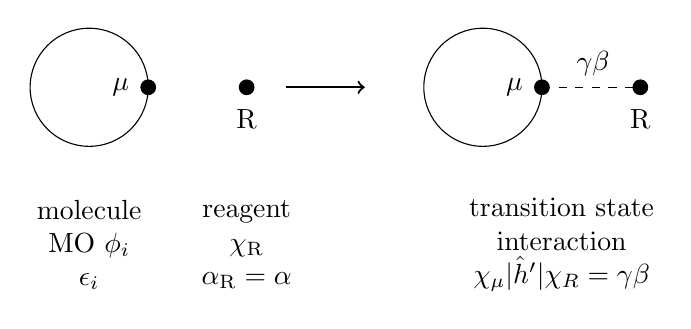
\begin{tikzpicture}
\draw (2,2) circle (0.75);
\fill[black] (2.75,2) circle (0.1);
\node at (2.4,2) {$\mu$};
\fill[black] (4,2) circle (0.1);
\node at (4,1.6) {R};
\draw[thick,->] (4.5,2) -- (5.5,2);
\draw (7,2) circle (0.75);
\fill[black] (7.75,2) circle (0.1);
\node at (7.4,2) {$\mu$};
\draw[dashed] (7.75,2) -- (9,2);
\fill[black] (9,2) circle (0.1);
\node at (9,1.6) {R};
\node at (8.4,2.3) {$\gamma\beta$};
\node[align=center] at (2,0) {molecule\\ MO $\phi_i$ \\$\epsilon_i$};
\node[align=center] at (4,0) {reagent\\ $\chi_\mathrm{R}$\\$\alpha_\mathrm{R} = \alpha$};
\node[align=center] at (8,0) {transition state \\ interaction \\ $\braket{\chi_\mu | \hat{h}'| \chi_R} = \gamma \beta$};
\end{tikzpicture}
\end{center}

%Recall that the second-order perturbation energy correction of the energy for an orbital $\psi_i$ due to a perturbation $\hat{h}'$ is given by
%\begin{equation}
%\Delta E_i^{(2)} = \sum_{k \neq i}^\text{unoccupied states} \frac{|\braket{\psi_i|\hat{h}'|\psi_k}|^2}{\epsilon_i - \epsilon_k},
%\end{equation}
%where $\hat{h}'$ contains the terms that describe the interaction between A and B.


Each  molecular orbital $\psi_i$ from H\"{u}ckel theory gets stabilized by an energy amount given by
\begin{equation}
\Delta E_i^{(2)} = \frac{|\braket{\psi_i|\hat{h}'|\chi_R}|^2}{\epsilon_i - \epsilon_R}.
\end{equation}
Note that there is no summation here because there is only one perturbing state (the empty orbital of the reagent). Here is a molecular orbital scheme that shows how the interaction of the reagent empty orbital stabilizes the orbitals in the transition state

\begin{center}
\includegraphics[width=3in]{../huckel/c2_reactivity_2.png}
\end{center}

The numerator of the expression for $\Delta E_i^{(2)}$ may be easily computed as
\begin{equation}
\braket{\psi_i|\hat{h}'|\chi_R} =\sum_\nu C_{\mu i} \braket{\chi_\nu|\hat{h}'|\chi_R}
 = C_{\mu i} \braket{\chi_\mu|\hat{h}'|\chi_R} = \gamma \beta C_{\mu i}.
\end{equation}
because $\psi_i = \sum_\mu^{N} \chi_\mu C_{\mu i}$ and only the matrix element $ \braket{\chi_\mu|\hat{h}'|\chi_R}$ is nonzero.
The denominator is instead given by
\begin{equation}
\epsilon_i - \epsilon_R = \alpha + \lambda_i \beta - \alpha = \lambda_i \beta,
\end{equation}
where we assumed that the electrophile is a carbon atom ($\epsilon_R = \alpha$).
Putting everything together we get
\begin{equation}
\Delta E_i^{(2)} = \frac{(\gamma \beta C_{\mu i})^2}{\lambda_i \beta} = \frac{C_{\mu i}^2}{\lambda_i} \gamma^2 \beta.
\end{equation}
If we sum this contribution over all the doubly occupied orbitals we get a total energy stabilization equal to 
\begin{equation}
2 \sum_i^\text{occ} \Delta E_i^{(2)} = 2 \sum_i^\text{occ} \frac{C_{\mu i}^2}{\lambda_i} \gamma^2 \beta
= S_R^\mathrm{E} \gamma^2 \beta.
\end{equation}
This equation partitions the interaction energy into a molecule specific part $S_R^\mathrm{E}$, called the \textit{superdelocalizability} and $\gamma^2 \beta$, a term that depends on the strength of the interaction.

The largest contribution to $S_R^\mathrm{E}$ comes form the MO with the smallest $|\lambda_i|$, which is called highest occupied molecular orbital (HOMO) and is given by the single term
\begin{equation}
2\frac{C_{\mu,\mathrm{HOMO}}^2}{\lambda_\mathrm{HOMO}}
\end{equation}
If we ignore the denominator we can consider a simplified reactivity index, the \textit{frontier electron density}, given by
\begin{equation}
f_\mu^\mathrm{El} = 2 C_{\mu,\mathrm{HOMO}}^2.
\end{equation}
The most reactive atom towards an electrophile is the one with the largest value of $f_\mu^\mathrm{El}$, among all possible values of $\mu$.
This means that the atom with the largest absolute coefficient in the HOMO is the most reactive.
One can repeat the same analysis for nucleophilic reactions, in which case the reactivity can be connected to a corresponding frontier electron density
\begin{equation}
f_\mu^\mathrm{Nuc} = 2 C_{\mu,\mathrm{LUMO}}^2,
\end{equation}
where LUMO indicates the lowest unoccupied MO.
These two indices allow to identify the atoms (labeled with $\mu$) with the highest reactivity towards electrophiles and nucleophiles by just looking at the HOMO and LUMO of a molecule.
For radical reactions, on considers instead the average of $f_\mu^\mathrm{El}$ and $f_R^\mathrm{Nuc}$
\begin{equation}
f_\mu^\mathrm{Rad} = \frac{1}{2} ( f_\mu^\mathrm{El} + f_\mu^\mathrm{Nuc} ).
\end{equation}

\section{Two-center interactions}
Another important application of H\"{u}ckel theory is in reactions that involve two centers, like cyclization of unsaturated hydrocarbons.
If we now consider two molecules, A and B, with centers $\mu$ and $\nu$ on A interacting with centers $\mu'$ and $\nu'$ on B, we can ask how much is the energy of the complex A + B stabilized by the interaction of the frontier orbitals (HOMO/LUMO) on each fragment.
\begin{center}
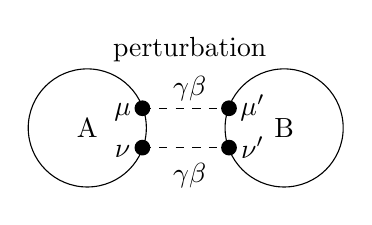
\begin{tikzpicture}
\draw (2,2) circle (0.75);
\draw (4.5,2) circle (0.75);
\fill[black] (2.7,2.25) circle (0.1);
\fill[black] (2.7,1.75) circle (0.1);
\fill[black] (3.8,2.25) circle (0.1);
\fill[black] (3.8,1.75) circle (0.1);
\draw[dashed] (2.7,2.25) -- (3.8,2.25);
\draw[dashed] (2.7,1.75) -- (3.8,1.75);
\node at (2.45,2.2) {$\mu$};
\node at (2.45,1.7) {$\nu$};
\node at (4.1,2.25) {$\mu'$};
\node at (4.1,1.75) {$\nu'$};
\node at (2,2) {A};
\node at (4.5,2) {B};
\node at (3.3,3.0) {perturbation};
\node at (3.3,2.5) {$\gamma\beta$};
\node at (3.3,1.4) {$\gamma\beta$};
\end{tikzpicture}
\end{center}

Assuming again that each pair of orbitals interacts with a term equal to $\gamma \beta$, we can write
\begin{equation}
\begin{split}
\braket{\chi_\mu | \hat{h}'| \chi_{\mu'}} = \gamma \beta, \\
\braket{\chi_\nu | \hat{h}'| \chi_{\nu'}} = \gamma \beta.
\end{split}
\end{equation}



Each orbital $\psi_i^\mathrm{A}$ on A will be stabilized by the interaction with the unoccupied orbitals on B
\begin{equation}
\Delta E_i^{\mathrm{A},(2)} = \sum_{k \neq i}^\text{virtual B} \frac{|\braket{\psi^\mathrm{A}_i|\hat{h}'|\psi^\mathrm{B}_k}|^2}{\epsilon^\mathrm{A}_i - \epsilon^\mathrm{B}_k}.
\end{equation}
Similarly, an orbital $\psi_i^\mathrm{B}$ on B will be stabilized by the interaction with the unoccupied orbitals on A by an amount
\begin{equation}
\Delta E_i^{\mathrm{B},(2)} = \sum_{k \neq i}^\text{virtual B} \frac{|\braket{\psi^\mathrm{B}_i|\hat{h}'|\psi^\mathrm{A}_k}|^2}{\epsilon^\mathrm{B}_i - \epsilon^\mathrm{A}_k}.
\end{equation}
Now let us suppose that the most important contribution comes from the interaction of the HOMO on A with the LUMO on B. The numerator for this contribution is given by
\begin{equation}
\Delta E_\mathrm{HOMO}^{\mathrm{A},(2)} = \frac{|\braket{\psi^\mathrm{A}_{\mathrm{HOMO}}|\hat{h}'|\psi^\mathrm{B}_{\mathrm{LUMO}}}|^2}{\epsilon^\mathrm{A}_{\mathrm{HOMO}}- \epsilon^\mathrm{B}_{\mathrm{LUMO}}}.
\end{equation}
If we plug in the definition of these two orbitals we get for the numerator
\begin{equation}
\begin{split}
\braket{\psi^\mathrm{A}_{\mathrm{HOMO}}|\hat{h}'|\psi^\mathrm{B_{\mathrm{LUMO}}}} &=
\sum_{\rho\sigma} 
\braket{\chi_\rho|\hat{h}'|\chi_\sigma}
C_{\rho,\mathrm{HOMO}}^\mathrm{A} C_{\sigma,\mathrm{LUMO}}^\mathrm{B} \\
&=
\braket{\chi_\mu|\hat{h}'|\chi_{\mu'}}
C_{\mu,\mathrm{HOMO}}^\mathrm{A} C_{\mu',\mathrm{LUMO}}^\mathrm{B}
+\braket{\chi_\nu|\hat{h}'|\chi_{\nu'}}
C_{\nu,\mathrm{HOMO}}^\mathrm{A} C_{\nu',\mathrm{LUMO}}^\mathrm{B}
\\
&=
\gamma\beta \underbrace{(
C_{\mu,\mathrm{HOMO}}^\mathrm{A} C_{\mu',\mathrm{LUMO}}^\mathrm{B}
+
C_{\nu,\mathrm{HOMO}}^\mathrm{A} C_{\nu',\mathrm{LUMO}}^\mathrm{B}
)}_{\delta}
=
\gamma\beta\delta
\end{split}
\end{equation}
We can now use this result to analyze the cyclization reaction between two molecules.

\section{Cyclization Reaction Between Two Molecules}
Consider the case of the HOMO of butadiene interacting with the LUMO of ethylene. In this case we can use simple symmetry considerations to learn something about the interaction of these two molecules in a cyclization reaction. The following plot show the HOMO and LUMO of butadiene and ethylene

\begin{center}
\includegraphics[width=3in]{../huckel/c2_cyclization_1.png}
\end{center}

For butadiene (A) the HOMO is antisymmetric, that is, it takes values with opposite signs on the two interacting atoms
\begin{equation}
C_{\mu,\mathrm{HOMO}}^\mathrm{A} = -C_{\nu,\mathrm{HOMO}}^\mathrm{A}
\end{equation}
and this is also true for the LUMO of ethylene (B)
\begin{equation}
C_{\mu',\mathrm{LUMO}}^\mathrm{B} = -C_{\nu',\mathrm{LUMO}}^\mathrm{B}.
\end{equation}
Taking these results into considerations we obtain
\begin{equation}
\delta = C_{\mu,\mathrm{HOMO}}^\mathrm{A} C_{\mu',\mathrm{LUMO}}^\mathrm{B}
+
C_{\nu,\mathrm{HOMO}}^\mathrm{A} C_{\nu',\mathrm{LUMO}}^\mathrm{B}
= 
2 C_{\mu,\mathrm{HOMO}}^\mathrm{A} C_{\mu',\mathrm{LUMO}}^\mathrm{B}
\end{equation}
This interaction leads to a lowering in energy since ${\epsilon^\mathrm{A}_{\mathrm{HOMO}}- \epsilon^\mathrm{B}_{\mathrm{LUMO}}} < 0$, therefore, we say that this interaction is \textbf{allowed}.
In general, the interaction of orbitals with the same symmetry is allowed.
For example, the interaction of the butadiene LUMO with the ethylene HOMO (the opposite of what we considered above) is a case where both orbitals are symmetric since
\begin{equation}
C_{\mu,\mathrm{LUMO}}^\mathrm{A} = C_{\nu,\mathrm{LUMO}}^\mathrm{A},
\end{equation}
and
\begin{equation}
C_{\mu',\mathrm{HOMO}}^\mathrm{B} = C_{\nu',\mathrm{HOMO}}^\mathrm{B}.
\end{equation}
For this case the quantity $\delta$ is also nonzero
\begin{equation}
\delta = 2 C_{\mu,\mathrm{LUMO}}^\mathrm{A} C_{\mu',\mathrm{HOMO}}^\mathrm{B}
\end{equation}

The interaction of two ethylene molecules is an example where the HOMO and LUMO have different symmetry

\includegraphics[width=3in]{../huckel/c2_cyclization_2.png}

In this case since
\begin{equation}
C_{\mu,\mathrm{HOMO}}^\mathrm{A} = C_{\nu,\mathrm{HOMO}}^\mathrm{A},
\end{equation}
and
\begin{equation}
C_{\mu',\mathrm{LUMO}}^\mathrm{B} = - C_{\nu',\mathrm{LUMO}}^\mathrm{B}.
\end{equation}
we find that $\delta = 0$.
This means that the interaction between orbitals of different symmetry is \textbf{forbidden}.
For general polyenes one has the following result:
\begin{equation}
(4n + 2) + (4n') \rightarrow 4 n'' + 2 \quad \text{symmetry allowed},
\end{equation}
while
\begin{equation}
\begin{split}
(4n + 2) + (4n' + 2) & \rightarrow 4 n'' +4\quad \text{forbidden}, \\
(4n) + (4n') & \rightarrow 4 n''\quad \text{forbidden}.
\end{split}
\end{equation}


\section{Orbital mixing rules}
Let's consider two atomic orbitals $\psi_i$ and $\psi_j$ and let them interact by, for example, bringing them together.
The interacting orbitals may be described by a two by two matrix of the form
\begin{equation}
\mathbf{h} = 
\begin{pmatrix}
\braket{\psi_i | \hat{h} |\psi_i} & \braket{\psi_i | \hat{h} |\psi_j} \\
\braket{\psi_j | \hat{h} |\psi_i} & \braket{\psi_j | \hat{h} |\psi_j}
\end{pmatrix}
=
\begin{pmatrix}
\epsilon_i & v \\
v & \epsilon_j
\end{pmatrix}.
\end{equation}

By examining the properties of the eigenvalues/eigenvectors of this matrix we can deduce some useful rules that can help us predict how orbitals mix.

\begin{itemize}
\item \textbf{Rule 1}. A pair of orbitals with zero overlap (orthogonal) do not mix. This is the case $v=0$, which basically means that the two orbitals do not interact due to symmetry.

\includegraphics[width=3in]{../huckel/c2_mix_rule_1.png}

\item \textbf{Rule 2}. When a pair of orbitals interact, they form a bonding (in-phase) orbital and an anti-bonding (out-of-phase) orbital. The bonding orbital is lower in energy than the antibonding orbital.

\includegraphics[width=2in]{../huckel/c2_mix_rule_2.png}

This rule follows from the equation for the eigenvalues of $\mathbf{h}$
\begin{equation}
\lambda_\pm = \frac{1}{2} (\epsilon_i + \epsilon_j)
\pm \frac{1}{2} \sqrt{(\epsilon_i - \epsilon_j)^2 + 4 v^2}.
\end{equation}
%Suppose $\epsilon_i \geq \epsilon_j$,
%The lowest eigenvalue ($\lambda_-$) corresponds to the eigenvector
%\begin{equation}
%v_1 = (\frac{\epsilon_i-\epsilon_j - \sqrt{(\epsilon_i - \epsilon_j)^2 + 4 v^2} }{2v} ,1)
%\end{equation}

\item \textbf{Rule 3}.  When the energy difference between a pair of orbitals before mixing is small and/or the overlap between a pair of orbitals is large, the energy separation becomes large after mixing.

\includegraphics[width=4in]{../huckel/c2_mix_rule_3.png}

\item \textbf{Rule 4}.  When a pair of orbitals with different energies interact, the newly formed MO has large contribution of the original orbital whose energy is closest to the newly formed MO.

\begin{center}
\includegraphics[width=4in]{../huckel/c2_mix_rule_4.png}
\end{center}


\item \textbf{Rule 5}. The same number of new MOs are created from the original orbitals before mixing ($N$ MOs from $N$ AOs).

\item \textbf{Rule 6}.    Suppose another orbital $\chi_c$ affects the two orbitals $\phi_1$  and $\phi_2$, which were formed mainly by interacting two orbitals $\chi_a$ and $\chi_b$.   The perturbation caused by the third orbital $\chi_c$ causes a small change of the orbital shape of $\phi_1$ and $\phi_2$.   When the energy of $\chi_c$ is higher than the energies of $\phi_1$ and $\phi_2$, the mixing of $\chi_c$ with $\phi_1$ and $\phi_2$ is in-phase.   When the energy of $\chi_c$ is lower than the energies of $\phi_1$ and $\phi_2$, the mixing of $\chi_c$ into $\phi_1$ and $\phi_2$ is out-of-phase.
 When three orbitals are interacting, the newly formed three MO's can be expressed with a linear combination of the original three orbitals.   The mixing coefficients depend on the energies of the original three orbitals.

\begin{center}
\includegraphics[width=4in]{../huckel/c2_mix_rule_6.png}
\end{center}
\end{itemize}


\section{Examples and Problems}
\subsection{Molecular orbitals of \ce{H3}}
Let us construct the molecular orbitals for the triangular and linear \ce{H3} species from the hydrogen atom and the molecular orbital of the \ce{H2} molecule. 

\textbf{Triangular \ce{H3}}

\begin{center}
\includegraphics[width=3in]{../huckel/c2_h3_tri.png}
\end{center}

 In the case of triangular \ce{H3}, let us assume that atomic hydrogen approaches on the bisecting axis of the hydrogen molecule.
 Note that $\chi_a$ interacts only with $\chi_b$ since the symmetry of $\chi_c$ is such that no mixing happens.
 The newly formed molecular orbital $\psi_1$ is the bonding combination between $\chi_a$ and $\chi_b$, and the molecular orbital $\psi_2$ is the corresponding anti-bonding combination. $\psi_3$ is the original $\chi_c$. 

\textbf{Linear \ce{H3}} (\ce{H. . . H-H})

\begin{center}
\includegraphics[width=3in]{../huckel/c2_h3_lin.png}
\end{center}

In the linear form of \ce{H3}, an hydrogen atom approaches the molecular axis of the hydrogen molecule.   The situation becomes different from the triangular \ce{H3} case, because all orbitals $\chi_a$, $\chi_b$, and $\chi_c$  interact with each other.
Comparing these two cases, we predict that the hydrogen exchange reaction \ce{H2 + H} prefers the linear transition-state structure since orbital interactions lead to an overall stabilization of the energy.

\begin{problem}[Molecular orbitals of \ce{H4}]
Construct the molecular orbitals for square \ce{H4} and linear \ce{H4} species from the two sets of molecular orbitals of the \ce{H2} molecule. 
Draw the orbital energy diagrams and discuss which structure is more stable.

\begin{center}
\includegraphics[width=2in]{../huckel/c2_problem_h4.png}
\end{center}

\end{problem}

\begin{problem}[$\pi$ MOs of benzene]
Create the six $\pi$-molecular orbitals of benzene by combining the two sets of $\pi$-orbitals of the allyl radical.   The picture shows only one side of $\pi$-plane (top view).

\begin{center}
\includegraphics[width=3in]{../huckel/c2_problem_benzene.png}
\end{center}

\end{problem}

%Once you know all the $\pi$-molecular orbitals of benzene, you can construct any -orbital of substituted benzene.   Let us make the HOMO (highest occupied molecular orbital) of phenol from benzene and the oxygen atom.
%   Assuming that the oxygen atom approaches to one of the carbon atoms of benzene along the C2v axis.   Before we construct the MOs of phenol, we should assign all of the unperturbed MOs under the C2v symmetry.   The MO of benzene does not interact with 2p-orbital of oxygen atom unless the symmetry of -MOs of benzene is b1 symmetry.   The HOMO of phenol 4 must be constructed from the anti-bonding combination between HOMO of the benzene 3 and the oxygen p-orbital o.   The second contributing orbital to the HOMO of phenol is the LUMO of benzene 5 which has a bonding combination with the oxygen p-orbital o.   We can neglect all other contributions from benzene -MO qualitatively, because the energy difference between 4 and 1 or 6 is larger than that between 4 and 3 or 5. 


 

 



\end{document}
%
%% This work is licensed under the Creative Commons Attribution-NonCommercial 4.0 International License.
% To view a copy of this license, visit http://creativecommons.org/licenses/by-nc/4.0/
% or send a letter to Creative Commons, PO Box 1866, Mountain View, CA 94042, USA.

% !TEX TS-program = xelatex

\documentclass[../Main/chem532-notes.tex]{subfiles}

\begin{document}

\chapter[The molecular Hamiltonian]{The molecular Hamiltonian and the Born--Oppenheimer approximation}

\section{Atomic Units}
When we study atoms and molecules, it is convenient to express positions, masses, and other properties in units that are close to one, so we can avoid carrying very large or small powers of 10.
The most common units used in quantum chemistry are \textbf{atomic units} (abbreviated a.u.). Atomic units are defined by the following conditions:
\begin{align}
\text{electron mass} & = m_e = 1\\
\text{electron charge} & = e = 1\\
\text{action} & = \hbar = \frac{h}{2\pi} = 1\\
\text{Coulomb's constant} & = k_e = \frac{1}{4\pi \epsilon_0} = 1
\end{align}
where $\epsilon_0$ is the vacuum permittivity.

The following table reports conversion factors between atomic units and other units 
\begin{table}[htbp]
\centering
\begin{tabular}{lll}
\toprule
Dimension & Symbol (Name) & Value in Other Units\\
\midrule
Length & $a_0$ (bohr) & 0.52918 \AA{} = 0.52918 $10^{-10}$ m\\ 
Mass & $m_e$ & $9.1095 \times 10^{-31}$ Kg \\
Charge & $e$ & $1.6022 \times 10^{-19}$ C \\
Action & $\hbar$ & $1.05457 \times 10^{-34}$ J $\cdot$ s \\
%Coulomb's constant & $\frac{1}{4\pi \epsilon_0}$ & $ \times 10^{-34}$ J $\cdot$ s \\
Energy & $E_{\rm h}$ (Hartree) & 627.51 kcal/mol \\
& & 27.211 eV \\
& & 219474.63 cm$^{-1}$ \\
& & $4.3598 \times 10^{-18}$ J\\
Time & & $2.41889 \times 10^{-17}$ s $\approx 1/41.3$ fs\\
\bottomrule
\end{tabular}
%\caption{Remember, \emph{never} use vertical lines in tables.}
\label{tab:atomicunits}
\end{table}

The speed of light in atomic units is $c = \alpha^{-1}\approx 137$ a.u.\mnote{$\alpha$ is the fine-structure constant $\alpha = \frac{e^2}{4\pi \epsilon_0 \hbar c}$ = 0.007 297 352 562 8(6), which in atomic units reduces to $\alpha = \frac{1}{c}$.}

\newpage

\section{The molecular Hamiltonian}
Consider a molecule containing $N$ electrons and $M$ nuclei.

\begin{center}
\includegraphics[width=2.5in]{../molecular-hamiltonian/coordinates.pdf}
\end{center}

We will start by introducing the notation used to define the molecular Hamiltonian.
The position of the nuclei will be indicated with $\vec{R}_A = \mathbf{R}_A = (x_A,y_A,z_A)$ and that of electrons with $\vec{r}_i = \mathbf{r}_i = (x_i,y_i,z_i)$.
The remaining quantities are summarized in the table below.
\begin{table}[h]
\centering
\begin{tabular}{lcc}
& Nuclei & Electrons \\
\hline
Total number & N & M \\
Index & $A, B, \ldots$ & $i, j, \ldots$ \\
Position & $\vec{R}_A$ & $\vec{r}_i$ \\
Mass & $M_A$ & $1$ \\
Charge & $Z_A$ & $-1$ \\
\end{tabular}
\end{table}

In the absence of external potentials or fields, the total Hamiltonian is given by
\begin{equation}
\hat{H} = \hat{T}_\mathrm{e} +\hat{T}_\mathrm{N} +  \hat{V}_\mathrm{ee} + \hat{V}_\mathrm{eN} + \hat{V}_\mathrm{NN},
\end{equation}
where
\begin{align}
\hat{T}_\mathrm{e} &= -\frac{\hbar^2}{2 m_e} \sum_i^N \nabla^2_i, \\
\hat{T}_\mathrm{N} &= -\frac{\hbar^2}{2} \sum_A^M \frac{1}{M_A} \nabla^2_A, \\
\hat{V}_\mathrm{ee} &= +\sum_{i}^{N}\sum_{j > i}^{N} \frac{1}{4 \pi \epsilon_0} \frac{e^2}{r_{ij}},\\
\hat{V}_\mathrm{eN} &= - \sum_{i}^{N} \sum_{A}^{M} \frac{1}{4 \pi \epsilon_0} \frac{e^2 Z_A}{r_{iA}}, \\
\hat{V}_\mathrm{NN} &= +\sum_{A}^{M} \sum_{B > A}^{M} \frac{1}{4 \pi \epsilon_0} \frac{e^2 Z_A Z_B}{r_{AB}},
\end{align}
and the quantity $r_{ij}$ is the distance between electrons labeled with indices $i$ and $j$
\begin{equation}
r_{ij} = |\vec{r}_i - \vec{r}_j| = \sqrt{(x_i-x_j)^2 + (y_i-y_j)^2 + (z_i-z_j)^2},
\end{equation}
and $r_{iA} = |\vec{r}_i - \vec{R}_A|$ and $r_{AB} = |\vec{R}_A - \vec{R}_B|$ are defined similarly.

In atomic units the Hamiltonian is more compact:
\begin{equation}
\label{eq:molecular_hamiltonian}
\hat{H} =
-\frac{1}{2} \sum_i^N \nabla^2_i
-\frac{1}{2} \sum_A^M \frac{1}{M_A} \nabla^2_A
+ \sum_{i}^{N}\sum_{j > i}^{N} \frac{1}{r_{ij}}
- \sum_{i}^{N} \sum_{A}^{M} \frac{Z_A}{r_{iA}}
+ \sum_{A}^{M} \sum_{B > A}^{M} \frac{Z_A Z_B}{r_{AB}},
\end{equation}
where $M_A$ is understood to be the mass of nucleus $A$ in atomic units.

If we define the collective electronic ($\mathbf{r} = \{ \vec{r}_i \}$) and nuclear ($\mathbf{R} = \{ \vec{R}_A \}$) degrees of freedom, we may write the Schr\"{o}dinger equation compactly as:
\begin{equation}
\hat{H} \Psi_k(\mathbf{r},\mathbf{R}) = E_k \Psi_k(\mathbf{r},\mathbf{R}).
\end{equation}

Note that $\Psi_k(\mathbf{r},\mathbf{R})$ is a complicated function of $3(N+M)$ variables (excluding spin) because it depends both on the coordinate of the electrons and nuclei. For a free molecule it includes translational, rotational, vibrational, and electronic degrees of freedom.
The terms that make this Hamiltonian difficult to solve are those that couple electrons and nuclei, that is, $\hat{V}_\mathrm{NN}$, $\hat{V}_\mathrm{eN}$, and $\hat{V}_\mathrm{eN}$ is problematic because it couples electrons and nuclei.

\begin{problem}	
What does the spectrum of $\hat{H}$ look like for a diatomic molecule?
\end{problem}


\section{Average value of the kinetic and potential energy}

The virial theorem can provide some useful constraints on the properties of stationary states.
%For the Hamiltonian
%\begin{equation}
%\hat{H} = \hat{T} + \hat{V}
%= \sum_i \frac{-1}{2 m_i} \nabla_i^2 + \hat{V}
%\end{equation}
Starting from the condition
\begin{equation}
\frac{d}{dt} \braket{\sum_p \vec{r}_p \hat{\vec{p}}_p} = 0,
\end{equation}
it is possible to show that if the potential $\hat{V} =  \hat{V}_\mathrm{ee} + \hat{V}_\mathrm{eN} + \hat{V}_\mathrm{NN}$ is a homogeneous function of order $k$,\mnote{A homogeneous function of order $k$, $f(\mathbf{x})$ is such that if we scale the argument by $s$ the function is scaled by $s^k$, that is $f(s \mathbf{x}) = s^k f(\mathbf{x})$.} then the expectation value of the kinetic and potential operators are related by
\begin{equation}
2 \braket{\hat{T}} -k \braket{\hat{V}} = 0.
\end{equation}
For Coulombic interactions $k = -1$ and so we have
\begin{equation}
\braket{\hat{V}} = -2 \braket{\hat{T}}.
\end{equation}
And
\begin{equation}
E = \braket{\hat{T}} + \braket{\hat{V}} = - \braket{\hat{T}} = \frac{\braket{\hat{V}}}{2} < 0.
\end{equation}


\section{The Born--Oppenheimer approximation}
One way to simplify the molecular Hamiltonian is to recognize that since electrons and nuclei have very different masses (the smallest value that $M_A$ can have is 1837 $m_e$, for the hydrogen atom) and treat the electronic and nuclear degrees of freedom separately.
More precisely, we are going to assume that we can break down the wave function into a product of an electronic wave function [$\Phi_{\mathrm{el}}(\mathbf{r};\mathbf{R})$] and a nuclear wave function [$\chi_{\mathrm{nuc}}(\mathbf{R})$]
\begin{equation}
\begin{split}
\Psi(\mathbf{r},\mathbf{R}) \approx \Phi_{\mathrm{el}}(\mathbf{r};\mathbf{R}) \chi_{\mathrm{nuc}}(\mathbf{R}).
\end{split}
\end{equation}
Note that the nuclear coordinates $\mathbf{R}$ enter in the electronic wave functions as a parameter, hence we use the symbol ``;'' to separate it from the electron coordinates $\mathbf{r}$. The nuclear wave function is instead independent of the electron coordinates; however, this does not mean that it will be independent from the electronic wave function (see later).

If we plug this trial state in the Schr\"{o}dinger equation, we get the following equation
\begin{equation}
\label{eq:schrodinger_equation_factorized_ansatz}
\begin{split}
(\hat{T}_\mathrm{e} + \hat{T}_\mathrm{N} + \hat{V}_\mathrm{ee} + \hat{V}_\mathrm{eN} +\hat{V}_\mathrm{NN}) \Phi_{\mathrm{el}}(\mathbf{r};\mathbf{R}) \chi_{\mathrm{nuc}}(\mathbf{R})
= E \Phi_{\mathrm{el}}(\mathbf{r};\mathbf{R}) \chi_{\mathrm{nuc}}(\mathbf{R})
\end{split}
\end{equation}
These five operators act on the wave function in different ways.
The kinetic energy operators take derivates with respect to coordinates, while the potential operators just multiply the wave function by a number.
The kinetic energy operator for the electrons acts only on the electronic coordinates and so we can write
\begin{equation}
\hat{T}_\mathrm{e} \Phi_{\mathrm{el}}(\mathbf{r};\mathbf{R}) \chi_{\mathrm{nuc}}(\mathbf{R})
= \chi_{\mathrm{nuc}}(\mathbf{R}) \hat{T}_\mathrm{e} \Phi_{\mathrm{el}}(\mathbf{r};\mathbf{R}).
\end{equation}
The nuclear kinetic energy operator complicates things a bit, because when we apply it to the wave function we get three terms
\begin{equation}
\begin{split}
\hat{T}_\mathrm{N}  \Phi_{\mathrm{el}}(\mathbf{r};\mathbf{R}) \chi_{\mathrm{nuc}}(\mathbf{R})
 = &  -\frac{1}{2} \sum_A^M \frac{1}{M_A} \nabla^2_A \left[  \Phi_{\mathrm{el}}(\mathbf{r};\mathbf{R}) \chi_{\mathrm{nuc}}(\mathbf{R}) \right] \\
= &  -\frac{1}{2} \sum_A^M \frac{1}{M_A}
\chi_{\mathrm{nuc}}(\mathbf{R})  \nabla^2_A  
\Phi_{\mathrm{el}}(\mathbf{r};\mathbf{R}) \\
& 
 - \sum_A^M \frac{1}{M_A}
 \nabla_A\chi_{\mathrm{nuc}}(\mathbf{R})  \cdot \nabla_A  
\Phi_{\mathrm{el}}(\mathbf{r};\mathbf{R}) \\
& 
 -\frac{1}{2} \sum_A^M \frac{1}{M_A}
 \Phi_{\mathrm{el}}(\mathbf{r};\mathbf{R})  \nabla^2_A \chi_{\mathrm{nuc}}(\mathbf{R}).
\end{split}
\end{equation}
The first and second terms on the right hand side of this equation couple the electronic and nuclear degrees of freedom.
If we neglect them and keep only the last term,
\begin{equation}
\begin{split}
\hat{T}_\mathrm{N}  \Phi_{\mathrm{el}}(\mathbf{r};\mathbf{R}) \chi_{\mathrm{nuc}}(\mathbf{R})
\approx 
 -\frac{1}{2} \sum_A^M \frac{1}{M_A}
 \Phi_{\mathrm{el}}(\mathbf{r};\mathbf{R})  \nabla^2_A \chi_{\mathrm{nuc}}(\mathbf{R}).
\end{split}
\end{equation}
 we can rewrite the Schr\"{o}dinger equation as
\begin{equation}
\begin{split}
\Phi_{\mathrm{el}}(\mathbf{r};\mathbf{R})   \hat{T}_\mathrm{N} \chi_{\mathrm{nuc}}(\mathbf{R}) + \chi_{\mathrm{nuc}}(\mathbf{R}) (\hat{T}_\mathrm{e} + \hat{V}_\mathrm{ee} + \hat{V}_\mathrm{eN} +\hat{V}_\mathrm{NN}) \Phi_{\mathrm{el}}(\mathbf{r};\mathbf{R}) 
= E \Phi_{\mathrm{el}}(\mathbf{r};\mathbf{R}) \chi_{\mathrm{nuc}}(\mathbf{R})
\end{split}
\end{equation}
To get this expression we collected all the wave functions not affected by operators to the left side of each term. Next we collect all the terms in the following way
\begin{equation}
\begin{split}
\chi_{\mathrm{nuc}}(\mathbf{R})(\hat{T}_\mathrm{e} + \hat{V}_\mathrm{ee} + \hat{V}_\mathrm{eN} +\hat{V}_\mathrm{NN}) \Phi_{\mathrm{el}}(\mathbf{r};\mathbf{R}) 
=\Phi_{\mathrm{el}}(\mathbf{r};\mathbf{R})    ( E - \hat{ T}_\mathrm{N}) 
\chi_{\mathrm{nuc}}(\mathbf{R})
\end{split},
\end{equation}
and finally divide each side by $\Phi_{\mathrm{el}}(\mathbf{r};\mathbf{R})\chi_{\mathrm{nuc}}(\mathbf{R})$ to get
\begin{equation}
\label{eq:molecular_hamiltonian:bo_derivation}
\begin{split}
\frac{1}{\Phi_{\mathrm{el}}(\mathbf{r};\mathbf{R}) } (\hat{T}_\mathrm{e} + \hat{V}_\mathrm{ee} + \hat{V}_\mathrm{eN} +\hat{V}_\mathrm{NN}) \Phi_{\mathrm{el}}(\mathbf{r};\mathbf{R}) = \frac{1}{\chi_{\mathrm{nuc}}(\mathbf{R})
}  ( E - \hat{ T}_\mathrm{N}) 
\chi_{\mathrm{nuc}}(\mathbf{R})
\end{split}
\end{equation}
The left and right sides of this equation must be equal for any values of $\mathbf{r}$ and $\mathbf{R}$, but since the right side does not depend on $\mathbf{r}$, both sides must depend only the variable $\mathbf{R}$.
Let us call this quantity $V(\mathbf{R})$.
Then Eq.~\eqref{eq:molecular_hamiltonian:bo_derivation} corresponds to two set of conditions
\begin{equation}
\label{eq:molecular_hamiltonian:electronic_se}
(\hat{T}_\mathrm{e} + \hat{V}_\mathrm{ee} + \hat{V}_\mathrm{eN} +\hat{V}_\mathrm{NN} ) \Phi_{\mathrm{el}}(\mathbf{r};\mathbf{R}) = V(\mathbf{R}) \Phi_{\mathrm{el}}(\mathbf{r};\mathbf{R}),
\end{equation}
and
\begin{equation}
\label{eq:molecular_hamiltonian:nuclear_se}
[\hat{ T}_\mathrm{N} + V(\mathbf{R}) ] \chi_{\mathrm{nuc}}(\mathbf{R})  =E \chi_{\mathrm{nuc}}(\mathbf{R}).
\end{equation}

Eqs.~\eqref{eq:molecular_hamiltonian:electronic_se} and \eqref{eq:molecular_hamiltonian:nuclear_se} are coupled equations.
We can find their solution by first solving the Schr\"{o}dinger equation for the electrons assuming that the nuclei are fixed in space ($\mathbf{R}$ is a constant).
Eq.~\eqref{eq:molecular_hamiltonian:electronic_se} is equivalent to the following \textbf{electronic} Schr\"{o}dinger equation
\begin{equation}
\label{eq:molecular_hamiltonian:electronic_se2}
(\hat{H}_\mathrm{el} + \hat{V}_\mathrm{NN})\Phi_{\mathrm{el},k}(\mathbf{r};\mathbf{R})
= V_{k}(\mathbf{R}) \Phi_{\mathrm{el},k}(\mathbf{r};\mathbf{R}).
\end{equation}
where the \textbf{electronic} Hamiltonian ($\hat{H}_{\rm el}$) is defined as:
\begin{equation}
\hat{H}_\mathrm{el} = \hat{T}_\mathrm{e} + \hat{V}_\mathrm{eN} + \hat{V}_\mathrm{ee}.
\end{equation}
Note that there are multiple solutions of the electronic Schr\"{o}dinger equation, so different pairs of eigenvalues/eigenfunctions are labeled by the state index $k$, which can take the values 0, 1, \ldots. The state with $k = 0$  is called the \textbf{ground electronic state}, while states with $k > 0$ are \textbf{excited electronic states}.
The function $V_{k}(\mathbf{R})$ is commonly known as the \textbf{potential energy surface} (abbreviates as PES).
Note that $V_{k}(\mathbf{R})$ gives us the potential energy at a given molecular geometry $\mathbf{R}$ and therefore it describes a set of surfaces in $3M + 1$ dimensions (nuclear coordinates plus energy).

Note that since for a fixed geometry $\hat{V}_\mathrm{NN}$ is a constant (it depends only on the relative positions of the nuclei), we can in practice solve the following eigenvalue problem
\begin{equation}
\label{eq:molecular_hamiltonian:electronic_se3}
\hat{H}_\mathrm{el}\Phi_{\mathrm{el},k}(\mathbf{r};\mathbf{R})
= E_{\mathrm{el}, k}(\mathbf{R}) \Phi_{\mathrm{el},k}(\mathbf{r};\mathbf{R}).
\end{equation}
which has the same eigenfunctions [$\Phi_{\mathrm{el},k}(\mathbf{r};\mathbf{R})$] but different eigenvalues [$E_{\mathrm{el}, k}(\mathbf{R})$].
The quantity $E_{\mathrm{el}, k}(\mathbf{R})$ is also called the \textbf{electronic energy} and it is related to $V_{k}(\mathbf{R})$ via the equation
\begin{equation}
V_{k}(\mathbf{R}) = E_{\mathrm{el},k}(\mathbf{R}) + \sum_{A}^{M} \sum_{B > A}^{M} \frac{Z_A Z_B}{r_{AB}}.
\end{equation}


The concept of the potential energy surface is at the basis of many concepts used to describe molecules like, the molecular geometry, transition states, etc.
The equilibrium geometry of a molecule in a given electronic state $k$, $\mathbf{R}_\mathrm{eq}$, is defined as the minimum of $V_{k}(\mathbf{R})$, that is, the gradient of $V_{k}(\mathbf{R})$ at this geometry is zero
\begin{equation}
\left. \frac{\partial V_{k}(\mathbf{R})}{\partial \mathbf{R}} \right|_{\mathbf{R}= \mathbf{R}_\mathrm{eq}}= 0,
\end{equation}
and the curvature of $V_{k}(\mathbf{R})$ at $\mathbf{R}_\mathrm{eq}$ is positive (the eigenvalues of the second derivative matrix or Hessian are all positive).
Note that for a given electronic state the equilibrium geometry may be unique or there might be several minima with the same energy.
In certain cases, the ground state might not be a bound molecular state (e.g., for dications like \ce{Li_2^{2+}} the energy minimum corresponds to the molecule dissociated into two \ce{Li^{+}} atoms).

\begin{example}[Potential energy surface of H$_2^+$]
The following plot shows the contributions of the electronic energy ($E_\mathrm{el}$) and the nuclear repulsion energy ($V_\mathrm{NN}$) to the potential energy of the ground state of H$_2^+$.
\begin{center}
\includegraphics[width =4.5in]{../molecular-hamiltonian/h2+_pec.pdf}
\end{center}
\end{example}

Although there are $3M$ nuclear degrees of freedom (DOF), in absence of an external potential translations and rotations of a molecule do not change the value of $V_{k}(\mathbf{R})$. Therefore, the number of internal degrees of freedom that change the value of $V_{k}(\mathbf{R})$ is less than $3M$. For a non-linear molecule we have that
\begin{equation}
\text{internal DOF} = \underbrace{3 M}_{\text{total DOF}}
-\underbrace{3}_{\text{rotations}}
-\underbrace{3}_{\text{translations}} = 3M - 6,
\end{equation}
while for a linear molecule
\begin{equation}
\text{internal DOF} = \underbrace{3 M}_{\text{total DOF}}
-\underbrace{2}_{\text{rotations}}
-\underbrace{3}_{\text{translations}} =  3M - 5.
\end{equation}

\begin{example}[Diatomic molecule]
For a diatomic molecule there is $2\cdot3 - 5 = 1$ degrees of freedom. In this case $V_{k}(\mathbf{R})$ may be expressed in terms of the bond distance $R$ as $V_{k}(\mathbf{R})$. In this case we call these quantities \textbf{potential energy curves}.
\end{example}





%\begin{figure}[htbp]
%   \centering
%   \includegraphics[width=4.5in]{figures/ch2_pec.png}
%   \caption{example caption}
%   \label{fig:example}
%\end{figure}

\section{Avoided crossings}
In this section we discuss some properties of potential energy surfaces. We are particularly interested in understanding when two surfaces become degenerate, because in this case the Born--Oppenheimer approximation is no longer qualitatively correct.
Consider two electronic states $\tilde{\Phi}_1(\mathbf{R})$ and $\tilde{\Phi}_2(\mathbf{R})$ that are not eigenfunctions of the electronic Hamiltonian. When do the potential energy surfaces obtained by diagonalizing the Hamiltonian in this basis become degenerate? 

Let us write the electronic Hamiltonian in the general\mnote{Here we do not assume that $\tilde{\Phi}_1$ and $\tilde{\Phi}_2$ are eigenfunctions of the Hamiltonian.} basis $\{\tilde{\Phi}_1(\mathbf{R}),\tilde{\Phi}_2(\mathbf{R})\}$ omitting the dependence on the coordinate $\mathbf{R}$
\begin{equation}
\mathbf{H}_\mathrm{el} = 
\begin{pmatrix}
\bra{\tilde{\Phi}_1} \hat{H}_\mathrm{el} \ket{\tilde{\Phi}_1} & \bra{\tilde{\Phi}_1} \hat{H}_\mathrm{el} \ket{\tilde{\Phi}_2}\\
\bra{\tilde{\Phi}_2} \hat{H}_\mathrm{el} \ket{\tilde{\Phi}_1} & \bra{\tilde{\Phi}_2} \hat{H}_\mathrm{el} \ket{\tilde{\Phi}_2}
\end{pmatrix}
=
\begin{pmatrix}
\tilde{E}_{1} & V \\
V^* & \tilde{E}_{2}
\end{pmatrix},
\end{equation}
where we used the fact that the Hamiltonian is Hermitian.\mnote{Because the Hamiltonian is Hermitian we have that $\bra{\tilde{\Phi}_2} \hat{H} \ket{\tilde{\Phi}_1} = \bra{\tilde{\Phi}_1} \hat{H} \ket{\tilde{\Phi}_2}^* =  V^*$.}

The difference between the eigenvalues $E_1$ and $E_2$ of $\mathbf{H}_\mathrm{el}$ is
\begin{equation}
E_2 - E_1 = \sqrt{(\tilde{E}_{2}-\tilde{E}_{1})^2 + 4 |V|^2 }.
\end{equation}
From this equation we deduce that for $E_1$ and $E_2$ to be degenerate, the following conditions must be satisfied \textbf{simultaneously}:
\begin{align}
\label{eq:molecular_hamiltonian:conical_intersection1}
\tilde{E}_{1}(\mathbf{R}) &= \tilde{E}_{2}(\mathbf{R}), \\
\label{eq:molecular_hamiltonian:conical_intersection2}
|V(\mathbf{R})| &= 0,
\end{align}
that is, the states that form our basis must be degenerate and there should be no coupling.

In general, these two conditions are independent. So suppose we find a point $\mathbf{R}^*$ for which Eqs.\eqref{eq:molecular_hamiltonian:conical_intersection1}-\eqref{eq:molecular_hamiltonian:conical_intersection2} are satisfied, then we can ask what is the dimensionality of the space in which these two states are degenerate?
If we consider a system with $M$ atoms and assume that $|V|$ is not zero for all molecular geometries,\mnote{In other words, $|V|$ is only \textbf{accidentally zero}.} then the subset of molecular geometries for which two potential energy surfaces intersect has dimension $3M - 6 - 2 = 3M - 8$ for non-linear molecules and $3M - 5 - 2 = 3M - 7$ for linear molecules.
Here we subtract 2 from the number of degrees of freedom to account for the two constraints that must be satisfied for the levels to be degenerate.
This result tells us when a crossing can happen, and if a crossing can happen, it tells us what is the dimension of the space of degenerate electronic energies.

\begin{example}[Diatomic molecules]
For a diatomic molecule degenerate electronic states live in a $3 \cdot 2 - 7 = -1$ dimensional space.
That is, in general two curves do not cross.
However, if for some reason the coupling $|V| = 0$ for all bond lengths then only one of the two constraints applies.
In this case, degenerate electronic states live in a space of dimension $3 \cdot 2 - 6 = 0$, that is, there may be a finite set of points for which $E_2 = E_1$.
Typical examples of situations when $|V| = 0$ include states with different spin or spatial symmetry.  For example, the singlet and triplet states of H$_2$ are allowed to cross.
Crossings may also occur when two electronic states have different number of electrons.
\end{example}

\section{The nuclear Schr\"{o}dinger equation}
Given the eigenvalues and eigenfunctions of the electronic Hamiltonian, it is possible to obtain wave functions for the nuclei by solving the nuclear Schr\"{o}dinger equation:
\begin{equation}
\hat{H}_{{\rm nuc},k} \chi_{v,k}(\mathbf{R}) =  E_{v,k} \chi_{v,k}(\mathbf{R}),
\end{equation}
where $\hat{H}_{{\rm nuc},k}$ is the nuclear Hamiltonian for electronic state $k$:
\begin{equation}
\hat{H}_{{\rm nuc},k} = \hat{T}_{N} + V_{k}(\mathbf{R}).
\end{equation}
In this approximation, the nuclei experience a potential generated by the electrons plus the nuclear-nuclear repulsion:
\begin{equation}
V_{k}(\mathbf{R}) = \int d\mathbf{r} \; \Phi^*_{\mathrm{el},k} (\mathbf{r};\mathbf{R}) \hat{H}_\mathrm{el}(\mathbf{R}) \Phi_{\mathrm{el},k} (\mathbf{r};\mathbf{R}) + V_\mathrm{NN}(\mathbf{R}).
\end{equation}
This expression is an equivalent way to rewrite $V_{k}(\mathbf{R}) $, and it emphasizes the fact that the potential energy surface is the potential experienced by the nuclei after averaging the interaction with the electrons in the state $\Phi_{\mathrm{el},k} (\mathbf{r};\mathbf{R})$.

Note that the solutions of the nuclear Schr\"{o}dinger equation are \textbf{vibrational levels} of the electronic state $k$.
Since each electronic state has a different shape, the vibrational levels for two electronic states are, in general, different.
In this picture, the electrons react instantaneously to the motion of the nuclei, so the nuclei always see the electrons in a fully relaxed state (adiabatic approximation).
The BO approximation is thus valid when nuclear and electronic motion occur on different time (energy) scales. In practice, the BO approximation is accurate when electronic states are well separated from one another, and, conversely, it fails when two or more electronic states become near-degenerate.
The first corrections to the BO approximation enter at order $\lambda^6 = \left( \frac{m_e}{M} \right)^{3/2}$, which for the hydrogen atom are of the order of $1.3 \cdot 10^{-5}$ \Eh.

\begin{details}	
In deriving the nuclear Schr\"{o}dinger equation we have neglected two terms that arise from the kinetic energy operator for the nuclei. So what happens if we introduce these terms back but still assume the BO factorized wave function for the electrons + nuclei?
Let us go back to the Schr\"{o}dinger equation for the electrons and nuclei where we plugged in the factorized form of the wave function [see Eq.~\eqref{eq:schrodinger_equation_factorized_ansatz}] and left project with the state $\Phi_{\mathrm{el}}^*(\mathbf{r};\mathbf{R})$ and integrate over $\mathbf{r}$ (we momentarily omit the electronic state index $k$ in the next few equations). This gives us
\begin{equation}
\begin{split}
\bra{\Phi_{\mathrm{el}}(\mathbf{r};\mathbf{R})} (\hat{T}_\mathrm{e} + \hat{T}_\mathrm{N}   + \hat{V}_\mathrm{ee} + \hat{V}_\mathrm{eN} +\hat{V}_\mathrm{NN} ) \ket{\Phi_{\mathrm{el}}(\mathbf{r};\mathbf{R})}  \chi_{\mathrm{nuc}}(\mathbf{R})
= E \chi_{\mathrm{nuc}}(\mathbf{R}).
\end{split}
\end{equation}
Using the fact that $(\hat{T}_\mathrm{e} + \hat{V}_\mathrm{eN} + \hat{V}_\mathrm{ee} + \hat{V}_\mathrm{NN} ) \Phi_{\mathrm{el}}(\mathbf{r};\mathbf{R}) = V(\mathbf{R}) \Phi_{\mathrm{el}}(\mathbf{r};\mathbf{R})$, we can simplify this equation to
\begin{equation}
\label{eq:molecular_hamiltonian:diagonal_bo}
\begin{split}
\bra{\Phi_{\mathrm{el}}(\mathbf{r};\mathbf{R})} (\hat{T}_\mathrm{N} +V(\mathbf{R}) ) \ket{\Phi_{\mathrm{el}}(\mathbf{r};\mathbf{R})}  \chi_{\mathrm{nuc}}(\mathbf{R})
= E \chi_{\mathrm{nuc}}(\mathbf{R}).
\end{split}
\end{equation}
The left-hand-side of this equation can be written as the sum of three terms:
\begin{equation}
\begin{split}
& [\hat{T}_\mathrm{N} +V(\mathbf{R})]  \chi_{\mathrm{nuc}}(\mathbf{R})  \\
& 
-\frac{1}{2} \sum_A^M \frac{1}{M_A}
\underbrace{\braket{\Phi_{\mathrm{el}}(\mathbf{r};\mathbf{R})|\nabla_A \Phi_{\mathrm{el}}(\mathbf{r};\mathbf{R})}}_{\text{First-order derivative coupling}}  \cdot \nabla_A \chi_{\mathrm{nuc}}(\mathbf{R}) \\
& 
-\frac{1}{2} \chi_{\mathrm{nuc}}(\mathbf{R}) \sum_A^M \frac{1}{M_A} \underbrace{\braket{\Phi_{\mathrm{el}}(\mathbf{r};\mathbf{R}) |\nabla^2_A \Phi_{\mathrm{el}}(\mathbf{r};\mathbf{R})} }_{\text{Second-order derivative coupling}}  .
\end{split}
\end{equation}
The first term appears in the nuclear Schr\"{o}dinger equation that we have seen before, but the terms in the second and third lines are new.
These are the so-called \textbf{diagonal corrections to the BO approximation} since they involve derivative couplings between the same electronic state.
These terms can be included in the nuclear Schr\"{o}dinger equation [Eq.~\eqref{eq:molecular_hamiltonian:diagonal_bo}] to estimate corrections to the BO approximation.
For heavy nuclei these corrections are somewhat small and so are typically neglected. 
However, diagonal corrections are sometime included in highly-accurate computations.

To go beyond diagonal BO corrections one has to consider solutions to the molecular Hamiltonian that mix various electronic states.
Since at each value of $\mathbf{R}$ the eigenfunctions of the electronic Hamiltonian form a complete basis for the electrons, we can expand the full wave function (electrons plus nuclei) as
\begin{equation}
\label{eq:molecular_hamiltonian:mol_ham_fullci}
\begin{split}
\Psi(\mathbf{r},\mathbf{R}) = \sum_{k=0}^\infty \Phi_{\mathrm{el},k}(\mathbf{r};\mathbf{R}) \chi_{\mathrm{nuc},k}(\mathbf{R}).
\end{split}
\end{equation}
When this equation is substituted in the Schr\"{o}dinger equation it leads to a set of coupled Schr\"{o}dinger  equations that determine the nuclear wave functions $\chi_{\mathrm{nuc},k}(\mathbf{R})$.
Note, however, that these nuclear wave functions are different from the ones we have encountered before.

Eq.~\eqref{eq:molecular_hamiltonian:mol_ham_fullci}  is the most general solution that we can write for a wave function of electrons and nuclei, and it is required when the assumptions made in the Born--Oppenheimer approximation are not valid.
A large number of interesting and important phenomena are associated with the break down of the adiabatic assumption and require a significantly more refined treatment than the one discussed here.
\end{details}
We will come back to the nuclear Schr\"{o}dinger equation after learning how to compute potential energy surfaces.
%

\section*{Study Questions}
\begin{myenumerate}
\item What are atomic units?
\item What is the unit of energy in atomic units?
\item What are the five terms in the molecular Hamiltonian?
\item What how many dimensions does the wave function for the molecular Hamiltonian have?
\item What is the basis for the Born--Oppenheimer approximation?
\item What terms in the expression $\hat{T}_\mathrm{N}  \Phi_{\mathrm{el}}(\mathbf{r};\mathbf{R})$ are neglected when deriving the Born--Oppenheimer approximation?
\item What is the electronic Schr\"{o}dinger equation?
\item What is the electronic Hamiltonian and what operators enter it?
\item What is the difference between the potential energy surface and the electronic energy?
\item Why do Eqs.~\eqref{eq:molecular_hamiltonian:electronic_se2} and \eqref{eq:molecular_hamiltonian:electronic_se3} share the same eigenfunction?
\item How many internal degrees of freedom are there for a linear and a nonlinear molecule?
\item Can two electronic state of the same symmetry cross in a diatomic molecule? What happens if the have the same symmetry?
\item What is the nuclear Schr\"{o}dinger equation?
\item Why do the solutions of the nuclear Schr\"{o}dinger equation depend on the electronic state?
\item What are the diagonal corrections to the BO approximation?
\end{myenumerate}

\end{document}
%
%% This work is licensed under the Creative Commons Attribution-NonCommercial 4.0 International License.
% To view a copy of this license, visit http://creativecommons.org/licenses/by-nc/4.0/
% or send a letter to Creative Commons, PO Box 1866, Mountain View, CA 94042, USA.

% !TEX TS-program = xelatex

\documentclass[../Main/chem532-notes.tex]{subfiles}
\begin{document}

\chapter{Electronic wave functions}

\section{Spin}
So far we have neglected to account for spin.
To introduce spin, we consider a set of spin operators $\hat{s}_x, \hat{s}_y, \hat{s}_z$, analogous to angular momentum operators.\mnote{We use lower case $s$ for spin operators that act only on one particle. This notation will help us distinguish from the spin operators for a collection of electrons.}
The spin operators satisfy the following commutation relationship
\begin{equation}
[\hat{s}_{j},\hat{s}_{k}] = \hat{s}_{j}\hat{s}_{k} - \hat{s}_{k}\hat{s}_{j}= i \hbar \varepsilon_{jkl} \hat{s}_{l} \quad \text{ with } j,k,l \in \{x,y,z\},
\end{equation}
where $\varepsilon_{jkl}$ is the Levi-Civita symbol defined as
\begin{equation}
\varepsilon_{jkl} = \begin{cases}
+1 & \text{if $(j,k,l)$ is an even permutation of $(x,y,z)$} \\
-1 & \text{if $(j,k,l)$ is an odd permutation of $(x,y,z)$} \\
0 & \text{otherwise}.
\end{cases}
\end{equation}

The total spin operator $\hat{\vec{s}}$ is a vector operator with components
\begin{equation}
\hat{\vec{s}} = (\hat{s}_x, \hat{s}_y, \hat{s}_z).
\end{equation}
We also define the angular momentum squared operator ($\hat{s}^2$) as
\begin{equation}
\hat{s}^2 = \hat{\vec{s}} \cdot \hat{\vec{s}} = \hat{s}_x^2 + \hat{s}_y^2 + \hat{s}_z^2.
\end{equation}
Since the $\hat{s}^2$ commutes with all vector components of $\hat{\vec{s}}$
\begin{equation}
[\hat{s}^2,\hat{s}_j] = 0 \quad \text{ with } j \in \{x,y,z\},
\end{equation}
we can pick one component, say the $z$ axis and introduce a basis of spin functions $\ket{s,m_s}$ that are simultaneous eigenfunctions of $\hat{s}^2$ and $\hat{s}_z$. Note that for a given value of $s$, $m_s$ can take values $s, s -1, s-2, \ldots, -s$.
The spin eigenfunctions satisfy:
\begin{align}
\hat{s}^2 \ket{s,m_s} &= \hbar^2 s(s+1), \\
\hat{s}_z \ket{s,m_s} &= \hbar m_s.
\end{align}

In the case of electrons we have that $s = \frac{1}{2}$, and so we label the two spin functions as $\alpha$ and $\beta$\mnote{Other notations are common. For example $\ket{0}$ and $\ket{1}$ is commonly used in quantum computing and $\ket{\uparrow}$ and $\ket{\downarrow}$ in physics.}
\begin{align}
\ket{\alpha} &= \ket{\frac{1}{2},\frac{1}{2}}, \\
\ket{\beta} &= \ket{\frac{1}{2},-\frac{1}{2}}.
\end{align}

These functions are normalized and orthogonal:
\begin{align}
\braket{\alpha | \alpha} &= \braket{\beta | \beta} = 1, \\
\braket{\alpha | \beta} &= 0. \label{eq:spin_orthogonality}
\end{align}
At times, we might write these functions as
\begin{align}
\alpha(\omega) &= \braket{\omega|\alpha} \\
\beta(\omega) &= \braket{\omega|\beta},
\end{align}
where $\omega$ is a fictitious spin variable. This allow us to treat $\alpha(\omega)$ and $\beta(\omega)$ as traditional wave functions. For example, the orthogonality condition [Eq.~\eqref{eq:spin_orthogonality}] may be written as
\begin{equation}
\braket{\alpha | \beta} = \int d\omega \, \alpha^*(\omega) \beta(\omega)  = 0.
\end{equation}

When talking about spin it is also convenient to introduce the raising ($\hat{s}_{+}$) and lowering ($\hat{s}_{-}$) spin operators.
These are defined as:
\begin{align}
\hat{s}_{+} & = \hat{s}_{x} + i \hat{s}_{y} \\
\hat{s}_{-} & = \hat{s}_{x} - i \hat{s}_{y}  
\end{align}
In the case of $s = \frac{1}{2}$ particles, the action of $\hat{s}_{+}$ and $\hat{s}_{-}$ on the spin eigenfunctions is
\begin{align}
\hat{s}_{+} \ket{\alpha} &= 0, \\
\hat{s}_{+} \ket{\beta} &= \ket{\alpha} \quad (m_s: -\frac{1}{2} \rightarrow \frac{1}{2}),\\
\hat{s}_{-} \ket{\alpha} &= \ket{\beta} \quad (m_s: \frac{1}{2} \rightarrow -\frac{1}{2}),\\
\hat{s}_{-} \ket{\beta} &= 0.
\end{align}
These operator raise or lower the value of $m_s$ or return zero if an eigenfunction with higher (lower) value of $m_s$ does not exist.
The $\hat{s}^2$ operator may be represented using the raising and lowering operators as
\begin{equation}
\hat{s}^2 = \hat{s}_{+}\hat{s}_{-} + \hat{s}^{2}_{z} - \hat{s}_{z}.
\end{equation}

It is also convenient to introduce many-electron generalizations of the spin operators.
For a system of $N$ electrons, we define total spin operators as the sum of operators action on each particle.
\begin{align}
\hat{S}^2 &= \sum_i^N \hat{s}^{2}(i), \\
\hat{S}_z &= \sum_i^N \hat{s}_{z}(i), \\
\hat{S}_+ &= \sum_i^N \hat{s}_{+}(i), \\
\hat{S}_- &= \sum_i^N \hat{s}_{-}(i),
\end{align}
where $\hat{s}^{2}(i)$ means that an operator $\hat{s}^{2}$ acts only on electron $i$.


\section{Spin orbitals}
Let us introduce some important nomenclature.
Functions that describe electrons in real space are called \textbf{spatial orbitals} and we will indicate them with the Greek symbol phi, $\phi_i(\vec{r})$.
In general the set $\{ \phi_i(\vec{r}) \}$ is infinite, complete, and may be orthonormalized.\mnote{A set of functions $\{ \phi_i(\vec{r}) \}$  is called \textbf{orthonormal} if any two functions satisfy $\int d\vec{r} \, \phi_i^*(\vec{r}) \phi_j(\vec{r})  = \delta_{ij}$.}
If the functions $\phi_i(\vec{r})$ are normalized then the quantity $|\phi_i(\vec{r})|^2 d\vec{r}$ is the probability of finding the electron in the volume element $d\vec{r}$.
The completeness condition implies that we can expand any function $f(\vec{r})$ using the set $\{ \phi_i(\vec{r}) \}$
\begin{equation}
f(\vec{r}) = \sum_{i}^{\infty} a_i \phi_i(\vec{r}).
\end{equation}
In practice, we use finite sets, so that $\dim \{ \phi_i(\vec{r}) \} = K < \infty$.

\textbf{Spin orbitals} are the product of a spatial orbital and a spin function:\mnote{We will abbreviate the spatial and spin coordinates with the symbol $x \equiv (\vec{r},\omega)$.}
\begin{equation}
\psi_{i,\sigma} (x) = \psi_{i,\sigma} (\vec{r},\omega) = \phi_i(\vec{r}) \sigma(\omega),
\end{equation}
where $\sigma(\omega) \in \{\alpha(\omega),\beta(\omega)\}$ indicates a generic spin function.
For a basis of spatial orbitals with dimension $K$ we can collect the indices $(i,\sigma)$ in one integer and define $2K$ spin orbitals:
\begin{align}
\psi_{2i - 1}(x) &= \phi_i(\vec{r}) \alpha(\omega), \\
\psi_{2i}(x) &= \phi_i(\vec{r}) \beta(\omega).
\end{align}
Note that if the spatial orbitals are orthonormal, then the spin orbital basis is also orthonormal:
\begin{equation}
\int d\vec{r} \, \psi_i^*(\vec{r}) \psi_j(\vec{r})  = \delta_{ij}.
\end{equation}


\section{$N$-electron wave functions}
How can we build a wave function for $N$ electrons $\Phi(x_1,x_2,\ldots,x_N)$ from a basis of spin orbitals? Pauli's principle requires that $\Phi$ is antisymmetric with respect to odd permutations of the coordinates (spatial and spin) of any two electrons $i$ and $j$:
\begin{equation}
\Phi(\ldots,x_i,\ldots,x_j,\ldots,x_N) = - \Phi(\ldots,x_j,\ldots,x_i,\ldots,x_N).
\end{equation}
Particles whose wave functions satisfies this condition are called \textbf{fermions}.

\begin{example}[Wave function for two electrons]
Consider a system of two electrons. The wave function is $\Phi(x_1,x_2)$ and the antisymmetry requirement is
\begin{equation}
 \Phi(x_2,x_1) = - \Phi(x_1,x_2).
\end{equation}
Now let us assume that we are given a complete spin orbital basis $\{ \psi_{i}(x) \}$.
We can think of $\Phi(x_1,x_2)$ with $x_2$ held constant as a function only of the variable $x_1$.
Therefore, we may expand $\Phi(x_1,x_2)$ using the spin orbital basis as:
\begin{equation}\label{eq:two_electron_wfn_expansion1}
\Phi(x_1,x_2) = \sum_{i}^{\infty} a_i(x_2) \psi_i(x_1),
\end{equation}
notice, however, that the expansions coefficients $a_i(x_2)$ will depend on the value of $x_2$, in other words, $a_i$ is a function of $x_2$.
We can now expand $a_i(x_2)$ using the same spin orbital basis:
\begin{equation}\label{eq:two_electron_wfn_expansion2}
a_i(x_2) = \sum_{j}^{\infty} a_{ij} \psi_j(x_2),
\end{equation}
and introduced the quantity $a_{ij}$, which carries both the indices for the $x_1$ and $x_2$ expansions.
Combining Eqs.~\eqref{eq:two_electron_wfn_expansion1}--\eqref{eq:two_electron_wfn_expansion2} we obtain:
\begin{equation}
\Phi(x_1,x_2) = \sum_{ij}^{\infty} a_{ij} \psi_i(x_1) \psi_j(x_2).
\end{equation}
This functions may satisfy the antisymmetry condition if:
\begin{equation}
\sum_{ij}^{\infty} a_{ij} \psi_i(x_1) \psi_j(x_2) = -\sum_{ij}^{\infty} a_{ij} \psi_i(x_2) \psi_j(x_1).
\end{equation}
To find out the implication of this condition onto the coefficients $a_{ij}$, first perform the index interchange $i \leftrightarrow j$ on the left hand side:
\begin{equation}
\sum_{ij}^{\infty} a_{ij} \psi_i(x_1) \psi_j(x_2) = -\sum_{ij}^{\infty} a_{ji} \psi_j(x_2) \psi_i(x_1),
\end{equation}
and the collect terms that multiply the factor $\psi_i(x_1) \psi_j(x_2)$ to obtain the condition:
\begin{equation}
\label{eq:two_electron_wfn_expansion4}
\sum_{ij}^{\infty} (a_{ij} + a_{ji}) \psi_i(x_1) \psi_j(x_2) = 0.
\end{equation}
Equation~\eqref{eq:two_electron_wfn_expansion4} must hold for any value of $\psi_i(x_1) \psi_j(x_2)$, and this is possible only if
\begin{equation} \label{eq:two_electron_wfn_expansion3}
a_{ij} + a_{ji} = 0.
\end{equation}
This conditions may also be written as 
\begin{equation}
a_{ij} = - a_{ji}.
\end{equation}
As a consequence, the diagonal elements of $a_{ij}$, $a_{ii}$, are zero.\mnote{To see this set $j = i$. Then $a_{ii} + a_{ii} = 2 a_{ii} = 0$, so that $a_{ii} = 0$.}
Eq.~\eqref{eq:two_electron_wfn_expansion3} shows that the when we expand an antisymmetric wave function using a single-particle basis, the antisymmetry condition is reflected in the properties of the coefficients $a_{ij}$.\mnote{The quantity $a_{ij}$ is a skew-symmetric or antisymmetric matrix. For $N$ electrons, the expansion coefficient will be an antisymmetric \textbf{tensor} with $N$ indices, that is $a_{i_1 i_2 i_3 \cdots i_N}$.}


Using Eq.~\eqref{eq:two_electron_wfn_expansion3} we may write the two-electron wave function as:
\begin{equation}
\begin{split}
\Phi(x_1,x_2) &= \sum_{i<j}^{\infty} a_{ij} \psi_i(x_1) \psi_j(x_2) + \sum_{i>j}^{\infty} a_{ij} \psi_i(x_1) \psi_j(x_2) \\
&= \sum_{i<j}^{\infty} a_{ij} \psi_i(x_1) \psi_j(x_2) + \sum_{j>i}^{\infty} a_{ji} \psi_j(x_1) \psi_i(x_2) \\
&= \sum_{i<j}^{\infty} a_{ij} \psi_i(x_1) \psi_j(x_2) - \sum_{i<j}^{\infty} a_{ij} \psi_i(x_2) \psi_j(x_1) \\
&= \sum_{i<j}^{\infty} a_{ij} [ \psi_i(x_1) \psi_j(x_2) - \psi_i(x_2) \psi_j(x_1)].
\end{split}
\end{equation}
The quantity $\psi_i(x_1) \psi_j(x_2) - \psi_i(x_2) \psi_j(x_1)$ can also be expressed as the determinant of a matrix since:
\begin{equation}
\det
\begin{bmatrix}
\psi_i(x_1) & \psi_i(x_2) \\
\psi_j(x_1) & \psi_j(x_2) 
\end{bmatrix}
\equiv
\begin{vmatrix}
\psi_i(x_1) & \psi_i(x_2) \\
\psi_j(x_1) & \psi_j(x_2) 
\end{vmatrix}
=
\psi_i(x_1) \psi_j(x_2) - \psi_i(x_2) \psi_j(x_1).
\end{equation}
Hence we discover that $\Phi(x_1,x_2)$ must be a linear combination of determinants:
\begin{equation}
\Phi(x_1,x_2) = \sum_{i<j}^{\infty} a_{ij} 
\begin{vmatrix}
\psi_i(x_1) & \psi_i(x_2) \\
\psi_j(x_1) & \psi_j(x_2)
\end{vmatrix}.
\end{equation}
\end{example}

A convenient way to represent antisymmetric wave functions for $N$ electrons is to expand it into a basis of functions that is automatically antisymmetric with respect to particle permutations. Such functions are known as \textbf{Slater determinants} and are defined as
\begin{equation}
\Phi_{ijk\cdots}(x_1,x_2,\ldots,x_N) = \frac{1}{\sqrt{N!}} 
\begin{vmatrix}
\psi_i(x_1) & \psi_i(x_2) & \cdots & \psi_i(x_N) \\
\psi_j(x_1) & \psi_j(x_2) & \cdots & \psi_j(x_N) \\
\psi_k(x_1) & \psi_k(x_2) & \cdots & \psi_k(x_N) \\
\vdots & \vdots & \vdots & \vdots
\end{vmatrix}.
\end{equation}
Slater determinants automatically satisfy the antisymmetry requirement of fermionic wave functions because the determinant of a matrix changes sign when two columns are swapped. This operation is equivalent to permuting particle indices.
For convenience we will write a Slater determinant, \textbf{including its normalization factor}, with the compact notation
\begin{equation}
\ket{\Phi_{ijk\cdots}} =\ket{
\psi_i \psi_j \psi_k \cdots},
\end{equation}
omitting the labels of the electrons.
The basis of Slater determinants $\{ \ket{
\psi_i \psi_j \psi_k \cdots} \}$ with $i, j, k, \ldots \in \{0, 1, 2, \ldots \}$ is complete.\mnote{This property is inherited from the fact that the one-electron spin orbital basis is complete.}
Therefore, we may expand any electronic wave function using the Slater determinant basis:
\begin{equation}
\ket{\Psi} = \sum_{i<j<k\cdots} C_{ijk\cdots} \ket{
\psi_i \psi_j \psi_k \cdots}.
\end{equation}
This expansion is called a \textbf{full configuration interaction} (FCI) wave function.
The FCI wave function can provide the exact solution to the electronic Schr\"{o}dinger equation.
In practice, we always work with a finite spin orbital basis. Then we say that the FCI wave function provides the exact solution of the Schr\"{o}dinger equation \textbf{within a finite basis}.
For a system with $N$ electrons and a spin orbital basis of dimension $2K$, the number of determinants in the FCI expansion is given by the number of ways to choose a subset of $N$ electrons, disregarding their order, from a set of $2K$ spin orbitals:
\begin{equation}
N_{\rm FCI} = \binom{2K}{N}.
\end{equation}
$N_{\rm FCI}$ grows very quickly with $N$ and $K$ and so the FCI wave function is impractical for more than 16--18 electrons.


\begin{example}[Hartree products vs. Slater determinants]
Let us compare a wave function that is just a product of spin orbitals with a Slater determinant for a two-electrons system.
A Hartree product is simply the product of orbitals:
\begin{equation}
\Phi^{\rm HP}(x_1,x_2) = \psi_i(x_1) \psi_j(x_2).
\end{equation}
The modulus square of $\Phi^{\rm HP}(x_1,x_2)$ shows that the probability distribution of two electrons is just the product of individual orbital probabilities:
\begin{equation}
| \Phi^{\rm HP}(x_1,x_2)|^2 = |\psi_i(x_1)|^2 |\psi_j(x_2)|^2 = P_i(x_1) P_j(x_2).
\end{equation}
A Hartree product represents a state with \textbf{no correlation}.

A Slater determinant:
\begin{equation}
\Phi^{\rm SD}(x_1,x_2) = \frac{1}{\sqrt{2}} [ \psi_i(x_1) \psi_j(x_2) - \psi_i(x_2) \psi_j(x_1)].
\end{equation}
has a probability distribution equal to:
\begin{equation}
\begin{split}
|\Phi^{\rm SD}(x_1,x_2)|^2 = \frac{1}{2} [&
P_i(x_1) P_j(x_2) +  P_j(x_1) P_i(x_2) \\
&-  \psi_i^*(x_1)\psi_j(x_1)  \psi_j^*(x_2) \psi_i(x_2)\\
&- \psi_j^*(x_1)\psi_i(x_1) \psi_j(x_2) \psi_i^*(x_2)  
].
\end{split}
\end{equation}
The first two terms are symmetrized probability distributions for individual orbitals [$P_i(x_1) P_j(x_2) +  P_j(x_1) P_i(x_2)$], while the third and fourth terms couple the position of electron 1 and 2.
If we integrate $|\Phi^{\rm SD}(x_1,x_2)|^2$ over the spin variables $\omega_1$ and $\omega_2$ we can derive a probability distribution that depends only on the positions of the electrons:
\begin{equation}
P(\mathbf{r}_1,\mathbf{r}_2) =
\int d\omega_1 d\omega_2 |\Phi^{\rm SD}(x_1,x_2)|^2.
\end{equation}
We now distinguish two cases.
If electrons have \textit{different} spin then the probability distribution is symmetric but not correlated:
\begin{equation}
P(\mathbf{r}_1,\mathbf{r}_2) = \frac{1}{2} [
P_i(\mathbf{r}_1) P_j(\mathbf{r}_2) +  P_j(\mathbf{r}_1) P_i(\mathbf{r}_2) ].
\end{equation}
If instead the two electrons have different spin, then the cross terms [$\psi_i^*(\mathbf{r}_1)\psi_j(\mathbf{r}_1)  \psi_j^*(\mathbf{r}_2) \psi_i(\mathbf{r}_2)$] survive and introduce correlation in the probability distribution
\begin{equation}
\begin{split}
P(\mathbf{r}_1,\mathbf{r}_2) = \frac{1}{2} [&
P_i(\mathbf{r}_1) P_j(\mathbf{r}_2) +  P_j(\mathbf{r}_1) P_i(\mathbf{r}_2) \\
&-  \phi_i^*(\mathbf{r}_1)\phi_j(\mathbf{r}_1)  \phi_j^*(\mathbf{r}_2) \phi_i(\mathbf{r}_2)\\
&- \phi_j^*(\mathbf{r}_1)\phi_i(\mathbf{r}_1) \phi_j(\mathbf{r}_2) \phi_i^*(\mathbf{r}_2)].
\end{split}
\end{equation}

We say that a Slater determinant accounts for \textbf{Fermi correlation}, a consequence of the antisymmetry of fermionic wave functions.
This form of correlation prevents two electrons with same spin to be found at the same point in space.
\end{example}

\section{Full configuration interaction wave function for H$_2$}
In this section we will do an extensive study of the wave function of H$_2$ in a minimal basis set.
Consider two hydrogen atoms (H$_\mathrm{A}$ and H$_\mathrm{B}$) separated by a distance $R_\mathrm{AB}$.
We will assume that each atom has one atomic basis function, $\chi_{1\rm s}^{\rm A}(\mathbf{r})$ and $\chi_{1\rm s}^{\rm B}(\mathbf{r})$.
Note that these two orbitals are not necessarily orthogonal as their overlap ($S$) is in general not equal to zero
\begin{equation}
S = \int d\mathbf{r} \chi_{1\rm s}^{\rm A}*(\mathbf{r}) \chi_{1\rm s}^{\rm B}(\mathbf{r}) \neq 0.
\end{equation}


From these atomic orbitals we can form two spatial orbitals:
\begin{align}
\phi_{\mathrm{g}}(\mathbf{r}) &= N_\mathrm{g} [\chi_{1\rm s}^{\rm A}(\mathbf{r}) + \chi_{1\rm s}^{\rm B}(\mathbf{r})],\\
\phi_{\mathrm{u}}(\mathbf{r}) &= N_\mathrm{u} [\chi_{1\rm s}^{\rm A}(\mathbf{r}) - \chi_{1\rm s}^{\rm B}(\mathbf{r})].
\end{align}

\begin{problem}[Normalization of the molecular orbitals of H$_2$]
Express the value of the normalization constants ($N_\mathrm{g}$ and $N_\mathrm{u}$) for the wave function $\phi_{\mathrm{g}}(\mathbf{r})$ and $\phi_{\mathrm{u}}(\mathbf{r})$ in terms of the overlap integral $S$. 
\end{problem}

By combining the spatial orbitals with spin functions we obtain four spin orbitals:
\begin{align}
\psi_1(x) = \psi_{\mathrm{g}}(x) = \phi_{\mathrm{g}}(\mathbf{r}) \alpha(\omega),\\
\psi_2(x) = \psi_{\bar{\mathrm{g}}}(x) = \phi_{\mathrm{g}}(\mathbf{r}) \beta(\omega),\\
\psi_3(x) = \psi_{\mathrm{u}}(x) = \phi_{\mathrm{u}}(\mathbf{r}) \alpha(\omega),\\
\psi_4(x) = \psi_{\bar{\mathrm{u}}}(x) = \phi_{\mathrm{u}}(\mathbf{r}) \beta(\omega).
\end{align}

From these spin orbitals we can form Slater determinants.
We cannot pick any pair of spin orbitals.
For example, the determinant:
\begin{equation}
\ket{\psi_{\mathrm{g}}\psi_{\mathrm{g}}} = 0,
\end{equation}
is zero because we have placed two electrons in the same spin orbital.\mnote{Just to avoid confusion: a spatial orbital may accommodate two electrons (with opposite spin) a spin orbitals can accommodate only one one electron.}
We may form six unique determinants:
\begin{align}
\ket{\Phi_1} = \ket{\psi_{\mathrm{g}}\psi_{\bar{\mathrm{g}}}} 
=
  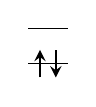
\begin{tikzpicture}[baseline={([yshift=-.5ex]current bounding box.center)},vertex/.style={anchor=base, minimum size=18pt, inner sep=2pt}]
    \draw (0,0.275) -- (0.5,0.275);
    \draw (0,0.725) -- (0.5,0.725);
    \draw[thick,->,>=stealth] (0.15,0.1) -- (0.15,0.45);
    \draw[thick,<-,>=stealth] (0.35,0.1) -- (0.35,0.45);
  \end{tikzpicture}\\[6pt]
  \ket{\Phi_2} = \ket{\psi_{\mathrm{g}}\psi_{\bar{\mathrm{u}}}} 
=
  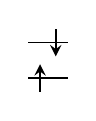
\begin{tikzpicture}[baseline={([yshift=-.5ex]current bounding box.center)},vertex/.style={anchor=base, minimum size=18pt, inner sep=2pt}]
    \draw (0,0.275) -- (0.5,0.275);
    \draw (0,0.725) -- (0.5,0.725);
    \draw[thick,->,>=stealth] (0.15,0.1) -- (0.15,0.45);
    \draw[thick,<-,>=stealth] (0.35,0.55) -- (0.35,0.9);
  \end{tikzpicture}\\[6pt]
  \ket{\Phi_3} = \ket{\psi_{\mathrm{u}}\psi_{\bar{\mathrm{g}}}} 
=
  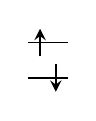
\begin{tikzpicture}[baseline={([yshift=-.5ex]current bounding box.center)},vertex/.style={anchor=base, minimum size=18pt, inner sep=2pt}]
    \draw (0,0.275) -- (0.5,0.275);
    \draw (0,0.725) -- (0.5,0.725);
    \draw[thick,<-,>=stealth] (0.35,0.1) -- (0.35,0.45);
    \draw[thick,->,>=stealth] (0.15,0.55) -- (0.15,0.9);
  \end{tikzpicture}\\[6pt]
    \ket{\Phi_4} = \ket{\psi_{\mathrm{u}}\psi_{\bar{\mathrm{u}}}} 
=
  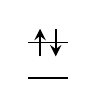
\begin{tikzpicture}[baseline={([yshift=-.5ex]current bounding box.center)},vertex/.style={anchor=base, minimum size=18pt, inner sep=2pt}]
    \draw (0,0.275) -- (0.5,0.275);
    \draw (0,0.725) -- (0.5,0.725);
    \draw[thick,<-,>=stealth] (0.35,0.55) -- (0.35,0.9);
    \draw[thick,->,>=stealth] (0.15,0.55) -- (0.15,0.9);
  \end{tikzpicture}\\[6pt]
      \ket{\Phi_5} = \ket{\psi_{\mathrm{g}}\psi_{\mathrm{u}}} 
=
  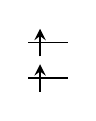
\begin{tikzpicture}[baseline={([yshift=-.5ex]current bounding box.center)},vertex/.style={anchor=base, minimum size=18pt, inner sep=2pt}]
    \draw (0,0.275) -- (0.5,0.275);
    \draw (0,0.725) -- (0.5,0.725);
    \draw[thick,->,>=stealth] (0.15,0.1) -- (0.15,0.45);
    \draw[thick,->,>=stealth] (0.15,0.55) -- (0.15,0.9);
  \end{tikzpicture}\\[6pt]
        \ket{\Phi_6} = \ket{\psi_{\bar{\mathrm{g}}}\psi_{\bar{\mathrm{u}}}} 
=
  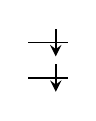
\begin{tikzpicture}[baseline={([yshift=-.5ex]current bounding box.center)},vertex/.style={anchor=base, minimum size=18pt, inner sep=2pt}]
    \draw (0,0.275) -- (0.5,0.275);
    \draw (0,0.725) -- (0.5,0.725);
    \draw[thick,<-,>=stealth] (0.35,0.55) -- (0.35,0.9);
    \draw[thick,<-,>=stealth] (0.35,0.1) -- (0.35,0.45);
  \end{tikzpicture}
\end{align}
Symmetry greatly simplifies this problem.\mnote{Recall that when an operator $\hat{O}$ commutes with the Hamiltonian, $[\hat{H},\hat{O}] = 0$, then it is possible to find a set of states that simultaneously diagonalize $\hat{H}$ and $\hat{O}$. For a set of symmetry operations this result implies that the eigensolutions of $\hat{H}$ may be classified according to the irreducible representations.}
The determinants $\ket{\Phi_1}$ and $\ket{\Phi_4}$ are gerade since the product $\psi_{\mathrm{g}}\psi_{\bar{\mathrm{g}}}$ has symmetry equal to g $\times$ g = g.\mnote{Recall that for molecules that possess a center of inversion the following rules apply: g $\times$ g = g, g $\times$ u = u $\times$ g = u, u $\times$ u = g.}
Determinants $\ket{\Phi_2}$, $\ket{\Phi_3}$, $\ket{\Phi_5}$, $\ket{\Phi_6}$ instead are ungerade.
Spin (which is another symmetry) helps.
Determinants 1--4 have all $M_S = 0$, while 5 and 6 have $M_S = +1$ and $-1$, respectively.
Determinants with different symmetry and spin will not contribute to the same eigenfunction.
As a consequence, the eigenfunctions for H$_2$ will be either a gerade state with $M_S = 0$ and wave function:
\begin{equation}
C_1 \ket{\Phi_1} + C_4 \ket{\Phi_4},
\end{equation}
or a ungerade state with $M_S = 0$ and wave function:
\begin{equation}
C_2 \ket{\Phi_2} + C_3 \ket{\Phi_3},
\end{equation}
or one of the two ungerade states with $M_S = \pm1$ ($\ket{\Phi_5}$, $\ket{\Phi_6}$).

Let us now analyze these determinants in terms of the atomic basis functions.
Consider $\Phi_1$, the lowest energy determinant.
If we plug in the definitions of the spin orbitals we obtain:
\begin{equation}
\begin{split}
\ket{\Phi_1} &= \ket{\psi_{\mathrm{g}} \psi_{\bar{\mathrm{g}}}} = N_{\mathrm{g}}^2 \ket{ (\chi_{1\rm s}^{\rm A} + \chi_{1\rm s}^{\rm B}) \alpha  (\chi_{1\rm s}^{\rm A} + \chi_{1\rm s}^{\rm B}) \beta} \\
&= N_{\mathrm{g}}^2 [ \ket{\chi_{1\rm s}^{\rm A}\alpha \chi_{1\rm s}^{\rm A}\beta}
+ \ket{\chi_{1\rm s}^{\rm A}\alpha \chi_{1\rm s}^{\rm B}\beta}
+ \ket{\chi_{1\rm s}^{\rm B}\alpha \chi_{1\rm s}^{\rm A}\beta} 
+\ket{\chi_{1\rm s}^{\rm B}\alpha \chi_{1\rm s}^{\rm B}\beta}].
\end{split}
\end{equation}
The first and last terms correspond to ionic configurations of electrons: 
\begin{equation}
 \ket{\chi_{1\rm s}^{\rm A}\alpha \chi_{1\rm s}^{\rm A}\beta} \equiv 
 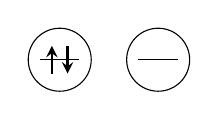
\begin{tikzpicture}[baseline={([yshift=-.5ex]current bounding box.center)},vertex/.style={anchor=base, minimum size=18pt, inner sep=2pt}]
    \draw (0.25,0.5) circle (0.4);
    \draw (0,0.5) -- (0.5,0.5);
    \draw[thick,->,>=stealth] (0.15,0.325) -- (0.15,0.675);
    \draw[thick,<-,>=stealth] (0.35,0.325) -- (0.35,0.675);    
    \draw (1.5,0.5) circle (0.4);
    \draw (1.25,0.5) -- (1.75,0.5);
  \end{tikzpicture}
\end{equation}
and
\begin{equation}
 \ket{\chi_{1\rm s}^{\rm B}\alpha \chi_{1\rm s}^{\rm B}\beta} \equiv 
 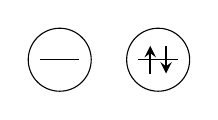
\begin{tikzpicture}[baseline={([yshift=-.5ex]current bounding box.center)},vertex/.style={anchor=base, minimum size=18pt, inner sep=2pt}]
    \draw (0.25,0.5) circle (0.4);
    \draw (0,0.5) -- (0.5,0.5);
    \draw[thick,->,>=stealth] (1.4,0.325) -- (1.4,0.675);
    \draw (1.5,0.5) circle (0.4);
    \draw (1.25,0.5) -- (1.75,0.5);
    \draw[thick,<-,>=stealth] (1.6,0.325) -- (1.6,0.675);
  \end{tikzpicture}
\end{equation}
since both electrons occupy the atomic orbitals on atom A or B.
The remaining contributions describe covalent bonds in which each atomic orbital is occupied with one electrons. These are:
\begin{equation}
 \ket{\chi_{1\rm s}^{\rm A}\alpha \chi_{1\rm s}^{\rm B}\beta} \equiv 
 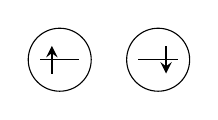
\begin{tikzpicture}[baseline={([yshift=-.5ex]current bounding box.center)},vertex/.style={anchor=base, minimum size=18pt, inner sep=2pt}]
    \draw (0.25,0.5) circle (0.4);
    \draw (0,0.5) -- (0.5,0.5);
    \draw[thick,->,>=stealth] (0.15,0.325) -- (0.15,0.675);
    \draw[thick,<-,>=stealth] (1.6,0.325) -- (1.6,0.675);
    \draw (1.5,0.5) circle (0.4);
    \draw (1.25,0.5) -- (1.75,0.5);
  \end{tikzpicture}
\end{equation}
and
\begin{equation}
 \ket{\chi_{1\rm s}^{\rm B}\alpha \chi_{1\rm s}^{\rm A}\beta} \equiv 
 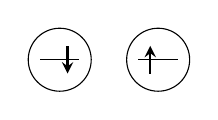
\begin{tikzpicture}[baseline={([yshift=-.5ex]current bounding box.center)},vertex/.style={anchor=base, minimum size=18pt, inner sep=2pt}]
    \draw (0.25,0.5) circle (0.4);
    \draw (0,0.5) -- (0.5,0.5);
    \draw[thick,<-,>=stealth] (0.35,0.325) -- (0.35,0.675);    
    \draw[thick,->,>=stealth] (1.4,0.325) -- (1.4,0.675);
    \draw (1.5,0.5) circle (0.4);
    \draw (1.25,0.5) -- (1.75,0.5);
  \end{tikzpicture}
\end{equation}
All these four determinants contribute equally, so the determinant $\Phi_1$ represents a state that has mixture of 50\% covalent and 50\% ionic electronic configurations.
The determinant $\Phi_4$ is also a 50/50 combination of covalent and ionic terms, but the sign of the covalent contributions is different:
\begin{equation}
\begin{split}
\ket{\Phi_4} &= \ket{\psi_{\mathrm{u}} \psi_{\bar{\mathrm{u}}}} = N_{\mathrm{u}}^2 \ket{ (\chi_{1\rm s}^{\rm A} - \chi_{1\rm s}^{\rm B}) \alpha  (\chi_{1\rm s}^{\rm A} - \chi_{1\rm s}^{\rm B}) \beta} \\
&= N_{\mathrm{u}}^2 [ \ket{\chi_{1\rm s}^{\rm A}\alpha \chi_{1\rm s}^{\rm A}\beta}
- \ket{\chi_{1\rm s}^{\rm A}\alpha \chi_{1\rm s}^{\rm B}\beta}
- \ket{\chi_{1\rm s}^{\rm B}\alpha \chi_{1\rm s}^{\rm A}\beta} 
+\ket{\chi_{1\rm s}^{\rm B}\alpha \chi_{1\rm s}^{\rm B}\beta}].
\end{split}
\end{equation}
Any linear combination of $\Phi_1$ and $\Phi_4$ may be used to represent covalent or ionic states because by carefully choosing $C_1$ and $C_4$ it is possible to cancel the ionic or covalent contributions.

The determinant $\Phi_5$ has $M_S = +1$ and is a component of a triplet state ($S = 1$).
Expanding $\Phi_5$ in terms of spin orbital we find:
\begin{equation}
\begin{split}
\ket{\Phi_5} &= \ket{\psi_{\mathrm{g}} \psi_{\mathrm{u}}} = N_{\mathrm{g}} N_{\mathrm{u}} \ket{ (\chi_{1\rm s}^{\rm A} + \chi_{1\rm s}^{\rm B}) \alpha  (\chi_{1\rm s}^{\rm A} - \chi_{1\rm s}^{\rm B}) \alpha} \\
&= N_{\mathrm{g}} N_{\mathrm{u}}  [
\underbrace{\ket{\chi_{1\rm s}^{\rm A}\alpha \chi_{1\rm s}^{\rm A}\alpha}}_{= 0}
- \ket{\chi_{1\rm s}^{\rm A}\alpha \chi_{1\rm s}^{\rm B}\alpha}
+ \ket{\chi_{1\rm s}^{\rm B}\alpha \chi_{1\rm s}^{\rm A}\alpha} 
- \underbrace{\ket{\chi_{1\rm s}^{\rm B}\alpha \chi_{1\rm s}^{\rm B}\alpha}}_{= 0}] \\
&= 2 N_{\mathrm{g}} N_{\mathrm{u}}  \ket{\chi_{1\rm s}^{\rm B}\alpha \chi_{1\rm s}^{\rm A}\alpha} .
\end{split}
\end{equation}
Where in the last step we used the antisymmetry property of Slater determinants and swapped the two spin orbitals
\begin{equation}
\ket{\chi_{1\rm s}^{\rm A}\alpha \chi_{1\rm s}^{\rm B}\alpha} = -\ket{\chi_{1\rm s}^{\rm B}\alpha \chi_{1\rm s}^{\rm A}\alpha}.
\end{equation}
We also eliminated the Pauli-principle violating terms like this:
\begin{equation}
 \ket{\chi_{1\rm s}^{\rm A}\alpha \chi_{1\rm s}^{\rm A}\alpha} \equiv 
 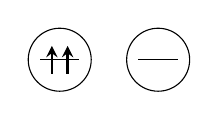
\begin{tikzpicture}[baseline={([yshift=-.5ex]current bounding box.center)},vertex/.style={anchor=base, minimum size=18pt, inner sep=2pt}]
    \draw (0.25,0.5) circle (0.4);
    \draw (0,0.5) -- (0.5,0.5);
    \draw[thick,->,>=stealth] (0.15,0.325) -- (0.15,0.675);
    \draw[thick,->,>=stealth] (0.35,0.325) -- (0.35,0.675);    
    \draw (1.5,0.5) circle (0.4);
    \draw (1.25,0.5) -- (1.75,0.5);
  \end{tikzpicture}
\end{equation}
In other words, this determinant accounts for Fermi correlation.
The state $\Phi_5$ corresponds to having each atomic orbital occupied by one alpha electron.

Finally, we will consider the spin of the determinants.
Apply the operator $\hat{S}^2$ to determinant $\Phi_5$:
\begin{equation}
\begin{split}
\hat{S}^2 \ket{\Phi_5} &= \hat{S}^2  \ket{\psi_{\mathrm{g}} \psi_{\mathrm{u}}} 
= (\hat{S}_{+} \hat{S}_{-}  + \hat{S}_{z}^2 - \hat{S}_{z}) \ket{\psi_{\mathrm{g}} \psi_{\mathrm{u}}}.
\end{split}
\end{equation}
Let us consider these terms in detail\mnote{$\hat{S}_{-}=\hat{s}_{-}(1) + \hat{s}_{-}(2)$.}
\begin{equation}
\hat{S}_{+} \hat{S}_{-} \ket{\psi_{\mathrm{g}} \psi_{\mathrm{u}}}
= \hat{S}_{+} (\ket{\psi_{\bar{\mathrm{g}}} \psi_{\mathrm{u}}} + \ket{\psi_{\mathrm{g}} \psi_{\bar{\mathrm{u}}}}
)
= 2 \ket{\psi_{\mathrm{g}} \psi_{\mathrm{u}}}.
\end{equation}
\begin{equation}
\hat{S}_{z} \ket{\psi_{\mathrm{g}} \psi_{\mathrm{u}}} = \left(\frac{1}{2} + \frac{1}{2}\right) \ket{\psi_{\mathrm{g}} \psi_{\mathrm{u}}} = \ket{\psi_{\mathrm{g}} \psi_{\mathrm{u}}}.
\end{equation}
Putting all together we get
\begin{equation}
\begin{split}
\hat{S}^2 \ket{\Phi_5} &= (\hat{S}_{+} \hat{S}_{-}  + \hat{S}_{z}^2 - \hat{S}_{z}) \ket{\psi_{\mathrm{g}} \psi_{\mathrm{u}}} \\
&= 2 \ket{\psi_{\mathrm{g}} \psi_{\mathrm{u}}} + \ket{\psi_{\mathrm{g}} \psi_{\mathrm{u}}} - \ket{\psi_{\mathrm{g}} \psi_{\mathrm{u}}} = 2 \ket{\psi_{\mathrm{g}} \psi_{\mathrm{u}}}.
\end{split}
\end{equation}
This result shows that $\Phi_5$ is an eigenfunction of $\hat{S}^2$ with eigenvalue equal to 2.
In other words, $S (S + 1) = 2$, which implies $S = 1$.
Therefore, $\Phi_5$ is the component of a triplet state with $M_S = +1$.
Since triplets are triply degenerate, there must be two other components of the triplet.
The $M_S = -1$ component is the determinant $\Phi_6$.

What about the $M_S = 0$ component?  It turns out that this component is contained in determinants $\Phi_2$ and $\Phi_3$.
Let us compute $\hat{S}^2 \ket{\Phi_2}$. We will need the quantity:
\begin{equation}
\begin{split}
\hat{S}_{+} \hat{S}_{-} \ket{\Phi_2}
= \hat{S}_{+} \hat{S}_{-} \ket{\psi_{\mathrm{g}}\psi_{\bar{\mathrm{u}}}}
= \hat{S}_{+} \ket{\psi_{\bar{\mathrm{g}}}\psi_{\bar{\mathrm{u}}}}
= \ket{\psi_{\mathrm{g}}\psi_{\bar{\mathrm{u}}}} + \ket{\psi_{\bar{\mathrm{g}}}\psi_{\mathrm{u}}}
\end{split},
\end{equation}
and
\begin{equation}
\hat{S}_{z} \ket{\psi_{\mathrm{g}}\psi_{\bar{\mathrm{u}}}}
= \left(\frac{1}{2} - \frac{1}{2}\right) \ket{\psi_{\mathrm{g}}\psi_{\bar{\mathrm{u}}}} = 0.
\end{equation}
From these results we find that:
\begin{equation}
\hat{S}^2 \ket{\Phi_2} = \ket{\psi_{\mathrm{g}}\psi_{\bar{\mathrm{u}}}} + \ket{\psi_{\bar{\mathrm{g}}}\psi_{\mathrm{u}}} 
= \ket{\psi_{\mathrm{g}}\psi_{\bar{\mathrm{u}}}} - \ket{\psi_{\mathrm{u}}\psi_{\bar{\mathrm{g}}}} = 
\ket{\Phi_2} - \ket{\Phi_3}.
\end{equation}
This means that $\Phi_2$ is not an eigenfunction of $\hat{S}^2$.
The fact that $\hat{S}^2 \ket{\Phi_2}$ gives back both $\Phi_2$ and $\Phi_3$ is a hint that a \textbf{linear combination} of these two determinants is an eigenfunction of spin.
The following result:
\begin{equation}
\hat{S}^2 \ket{\Phi_3} = \ket{\Phi_2} + \ket{\Phi_3}.
\end{equation}
suggests that we consider the plus and minus combination of $\Phi_2$ and $\Phi_3$:
\begin{equation}
\ket{\Phi_\pm} = \frac{1}{\sqrt{2}} \left(  \ket{\Phi_2} \pm \ket{\Phi_3} \right).
\end{equation}
These two states are such that
\begin{equation}
\hat{S}^2 \ket{\Phi_+} = 0,
\end{equation}
and
\begin{equation}
\hat{S}^2 \ket{\Phi_{-}} = 2 \ket{\Phi_{-}}.
\end{equation}
Therefore, $\Phi_{-}$ is a triplet state while $\Phi_{+}$ is a singlet state.

\end{document}
%
%% This work is licensed under the Creative Commons Attribution-NonCommercial 4.0 International License.
% To view a copy of this license, visit http://creativecommons.org/licenses/by-nc/4.0/
% or send a letter to Creative Commons, PO Box 1866, Mountain View, CA 94042, USA.

% !TEX TS-program = xelatex

\documentclass[../Main/chem532-notes.tex]{subfiles}
\begin{document}

\setcounter{chapter}{4}

\chapter{Hartree--Fock theory}

\section{The Hartree--Fock wave function}
The main assumption of Hartree--Fock theory is that the wave functions for $N$ electrons may be approximated with a single Slater determinant built from a set of ``optimal'' spin orbitals $\{ \psi_1, \psi_2, \ldots, \psi_N \}$:
\begin{equation}
\ket{\Phi_0} = \ket{\psi_1, \psi_2, \ldots, \psi_N }.
\end{equation}
The goal is to find the best set of spin orbitals in the variational sense. 
Let us define the functional $E[\Phi]$ of a trial wave function $\Phi$:
\begin{equation}
E[\Phi] = \bra{\Phi} \hat{H} \ket{\Phi},
\end{equation}
then the Hartree--Fock energy is given by:
\begin{equation}
E_0 = \min_{\Phi} E[\Phi] \quad \text{ enforcing }  \quad\braket{\Phi | \Phi} = 1,
\end{equation}
where we assume that the determinant $\Phi$ is normalized.

In a spin orbital basis the Hartree--Fock energy is:
\begin{equation}
E_0[\{ \psi_i \}] = \sum_i^{\rm occ} \bra{i} \hat{h} \ket{i} + \frac{1}{2} \sum_{ij}^{\rm occ} \aphystei{ij}{ij}.
\end{equation}


\subsection{Minimization of the Hartree--Fock energy functional}
As we have seen in the previous section, if the spin orbitals are orthonormal then $\Phi$ is guaranteed to be normalized.
How can we minimize the Hartree--Fock energy functional and at the same time impose the condition $\braket{\psi_i|\psi_j} = \delta_{ij}$?
We will use the technique of Lagrange multipliers.

\begin{example}[Minimization of a function of two variables with a constraint]
Let us consider the problem of minimizing the function $f(x,y) = x^2 + 2 y^2$ with the constraint that $x + y = 2$.
We rewrite the constraint as a function $g(x,y) = x + y - 2$ and we will try to impose $g(x,y) = 0$.
Consider the Lagrangian function of three independent variables $(x,y,\lambda)$:
\begin{equation}
\mathcal{L}(x,y,\lambda) = f(x,y) - \lambda g(x,y) =  x^2 + 2 y^2 - \lambda (x + y - 2).
\end{equation}
The stationary point of $\mathcal{L}(x,y,\lambda)$ with respect to the variables $x$, $y$, and $\lambda$ corresponds to:
\begin{align}
\frac{\partial \mathcal{L}(x,y,\lambda)}{\partial x} &= 2 x - \lambda = 0 \label{eq:hf:lagrange1}\\
\frac{\partial \mathcal{L}(x,y,\lambda)}{\partial y} &= 4 y - \lambda = 0 \label{eq:hf:lagrange2}\\
\frac{\partial \mathcal{L}(x,y,\lambda)}{\partial \lambda} &= g(x,y)  = 0.\label{eq:hf:lagrange3}
\end{align}
From Eqs.~\eqref{eq:hf:lagrange1} and \eqref{eq:hf:lagrange2} we obtain:
\begin{equation}
x = 2y,
\end{equation}
which combined with Eq.~\eqref{eq:hf:lagrange3} gives: 
\begin{equation}
g(2y,y)  = 2y + y - 2 = 0 \quad \Rightarrow \quad y = \frac{2}{3},
\end{equation}
and $x = \frac{4}{3}$.
\end{example}

To enforce orthonormality of the spin orbitals we need to enforce the condition:
\begin{equation}
\braket{\psi_i | \psi_j} = \delta_{ij} \quad \forall i,j \in \mathrm{occupied}.
\end{equation}
To enforce this constraint we consider the following Lagrangian:
\begin{equation}
\mathcal{L}[\{ \psi_i \}] = E_0[\{ \psi_i \}] - \sum_{ij}^\mathrm{occ} \lambda_{ji} (\braket{\psi_i | \psi_j} - \delta_{ij}),
\end{equation}
where $\lambda_{ji}$ is a matrix of Lagrange multipliers.\mnote{In writing the Lagrange multiplier we chose for convenience to put the index ``q'' before ``p''. This notation will be convenient later in the derivation.}
Note that $\lambda_{ji}$ must be a Hermitian matrix\mnote{That is $\lambda_{ji} = \lambda_{ji}^*$.}, which is a consequence of requiring the Lagrangian to be a real function.\mnote{A complex Lagrangian cannot be minimized because there is no such a thing as the minimum of a complex function.}
%Imposing 
%$\mathcal{L}[\{ \psi_i \}]  = \mathcal{L}[\{ \psi_i \}]^*$
%it follows that:
%\begin{equation}
%\sum_{ij}^\mathrm{occ} \lambda_{ji} (\braket{\psi_p}{\psi_q} - \delta_{pq})
%= \sum_{ij}^\mathrm{occ} \lambda_{ji}^* (\braket{\psi_p}{\psi_q} - \delta_{pq})
%\end{equation}
%
%\begin{equation}
%\sum_{ij}^\mathrm{occ} ( \lambda_{ji} -  \lambda_{ji}^* )(\braket{\psi_p}{\psi_q} - \delta_{pq}) = 0
%\end{equation}
To find the minimum of $\mathcal{L}[\{ \psi_i \}]$ we require that the Lagrangian is stationary with respect to small variations of the spin orbitals $\{ \delta \psi_i \}$.
This mean that for any arbitrary variation of the spin orbitals $\{ \delta \psi_i \}$ the Lagrangian must satisfy:
\begin{equation}
\mathcal{L}[\{ \psi_i  + \delta \psi_i \}] = \mathcal{L}[\{ \psi_i \}],\end{equation}
up to first order in $\{ \delta \psi_i \}$.
Let us first evaluate the variation of the energy:
\begin{equation}
\begin{split}
E_0[\{ \psi_i +  \delta \psi_i\}] =&
\sum_i^{\rm occ} \bra{\psi_i + \delta \psi_i} \hat{h} \ket{\psi_i + \delta \psi_i} \\
&+ \frac{1}{2} \sum_{ij}^{\rm occ} \aphystei{(\psi_i + \delta \psi_i) (\psi_j + \delta \psi_j)}{(\psi_i + \delta \psi_i) (j + \delta \psi_j)} \\
=& E_0[\{ \psi_i \}] + \sum_i^{\rm occ} \bra{\psi_i} \hat{h} \ket{\delta \psi_i}
+ \sum_i^{\rm occ} \bra{\delta \psi_i} \hat{h} \ket{\psi_i} \\
&+ \frac{1}{2} \sum_{ij}^{\rm occ} \aphystei{\delta \psi_i \psi_j}{\psi_i \psi_j}
+ \frac{1}{2} \sum_{ij}^{\rm occ} \aphystei{\psi_i \delta \psi_j}{\psi_i \psi_j} \\
&+ \frac{1}{2} \sum_{ij}^{\rm occ} \aphystei{\psi_i \psi_j}{\delta \psi_i \psi_j}
+ \frac{1}{2} \sum_{ij}^{\rm occ} \aphystei{\psi_i \psi_j}{\psi_i \delta \psi_j}\\
&+ \text{(higher order)} \\
=& E_0[\{ \psi_i \}] + \sum_i^{\rm occ} \left[ \bra{\delta \psi_i} \hat{h} \ket{\psi_i} 
+ \sum_{j}^{\rm occ} \aphystei{\delta \psi_i \psi_j}{\psi_i \psi_j} \right]\\&+ \text{h.c.} + \text{(higher order)},
\end{split}
\end{equation}
where ``h.c.'' stands for Hermitian conjugate.

The variation of the constraint $- \sum_{ij}^\mathrm{occ} \lambda_{ji} (\braket{\psi_p|\psi_q} - \delta_{pq})$ is equal to:
\begin{equation}
\begin{split}
- \sum_{ij}^\mathrm{occ} \lambda_{ji} (\braket{\psi_i + \delta \psi_i|\psi_j + \delta \psi_j} - \delta_{ij})
=& - \sum_{ij}^\mathrm{occ} \lambda_{ji} (\braket{\psi_i|\psi_j} - \delta_{ij}) \\
& - \sum_{ij}^\mathrm{occ} \lambda_{ji} \braket{\delta\psi_i|\psi_j}  - \sum_{ij}^\mathrm{occ} \lambda_{ji} \braket{\psi_i|\delta\psi_j} \\
&+ \text{(higher order)}.
\end{split}
\end{equation}

Let us identify the change in the Lagrangian up to linear terms, that is:
\begin{equation}
\delta \mathcal{L} = \mathcal{L}[\{ \psi_i  + \delta \psi_i \}] - \mathcal{L}[\{ \psi_i  \}]
\end{equation}

\begin{equation}
\begin{split}
\delta \mathcal{L}  =
\sum_i^{\rm occ} \left[ \bra{\delta \psi_i} \hat{h} \ket{\psi_i} 
+ \sum_{j}^{\rm occ} \aphystei{\delta \psi_i \psi_j}{\psi_i \psi_j} - \sum_{ij}^\mathrm{occ} \lambda_{ji} \braket{\delta\psi_p|\psi_q} \right] + \text{h.c.} 
\end{split}
\end{equation}

We now rewrite this expression in terms of integrals:
\begin{equation}
\begin{split}
\delta \mathcal{L}  =&
\sum_{i}^\mathrm{occ} \int dx_1 \delta\psi_{i}^{*}(x_1) \times \\
& \times
\left[
\hat{h}\psi_{i}(x_1) 
+ \sum_{j}^\mathrm{occ} \int dx_2 \frac{|\psi_{j}(x_2)|^2 \psi_{i}(x_1) }{|\mathbf{r}_1 - \mathbf{r}_2|}
- \sum_{j}^\mathrm{occ} \int dx_2 \frac{\psi_{j}^{*}(x_2) \psi_{i}(x_2) \psi_{j}(x_1) }{|\mathbf{r}_1 - \mathbf{r}_2|}
- \sum_{j}^\mathrm{occ} \lambda_{ji} \psi_{j}(x_1)
\right].
\end{split}
\end{equation}
If we require $\delta \mathcal{L}$ to be null for any variation of the orbitals then the quantity inside the square bracket must be identically null. We can write this condition in the following way, which is suggestive of a eigenvalue problem:
 \begin{equation}
\hat{h}\psi_{i}(x_1) 
+ \sum_{j}^\mathrm{occ} \int dx_2 \frac{|\psi_{j}(x_2)|^2 \psi_{i}(x_1) }{|\mathbf{r}_1 - \mathbf{r}_2|}
- \sum_{j}^\mathrm{occ} \int dx_2 \frac{\psi_{j}(x_2)^{*} \psi_{i}(x_2) \psi_{j}(x_1) }{|\mathbf{r}_1 - \mathbf{r}_2|}
= \sum_{j}^\mathrm{occ} \lambda_{ji} \psi_{j}(x_1).
\end{equation}
If we introduce the Coulomb ($\hat{J}_j$) and exchange ($\hat{K}_j$) operators:
\begin{align}
\hat{J}_j(x_1)\psi_{i}(x_1)  &= \int dx_2 \frac{|\psi_{j}(x_2)|^2}{|\mathbf{r}_1 - \mathbf{r}_2|} \psi_{i}(x_1) \\
\hat{K}_j(x_1)\psi_{i}(x_1)  &= \int dx_2 \frac{\psi_{j}^{*}(x_2) \psi_{i}(x_2)}{|\mathbf{r}_1 - \mathbf{r}_2|} \psi_{j}(x_1),
\end{align}
we may rewrite the stationary conditions as:
 \begin{equation}
\left[ \hat{h}(x_1) + \sum_{j}^\mathrm{occ} \hat{J}_j(x_1)- \hat{K}_j(x_1) \right] \psi_{i}(x_1) 
= \sum_{j}^\mathrm{occ} \lambda_{ji} \psi_{j}(x_1),
\end{equation}
or
\begin{equation} \label{eq:hf:noncanonical_hf_equation}
\hat{f}(x_1)  \psi_{i}(x_1) 
= \sum_{j}^\mathrm{occ} \lambda_{ji} \psi_{j}(x_1).
\end{equation}
Eq.~\eqref{eq:hf:noncanonical_hf_equation} is called the \textbf{Hartree--Fock equation in noncanonical form} and the operator $\hat{f}(x_1) = \hat{h}(x_1) + \sum_{j}^\mathrm{occ} \hat{J}_j(x_1)- \hat{K}_j(x_1)$ is called the Fock operator.
Note, that this is not an eigenvalue problem because on the r.h.s. we have a sum of functions.
Essentially this equations says that when we apply the Fock operator to any occupied orbital, we get back a linear combination of occupied orbitals.
This implies that if we apply the Fock operator to a unoccupied (virtual) orbital, then we get back a linear combination of virtual orbitals.

\subsection{Hartree--Fock equations in the canonical form}
Consider a unitary transformation of the occupied orbitals:
\begin{equation}
\ket{\psi'_i} = \sum_{j}^\mathrm{occ} \ket{\psi_j} U_{ji},
\end{equation}
where the matrix $\mathbf{U}$ is unitary.\mnote{$\mathbf{U}^{-1} = \mathbf{U}^{\dagger}$}
It is possible to prove that a determinant built from the spin orbitals $\psi'_i$ is related to the determinant in the original basis by a complex phase factor:
\begin{equation}
\ket{\Phi'} = \ket{\psi'_1 \psi'_2 \cdots \psi'_N} = e^{i\theta} \ket{\Phi}.
\end{equation}
From this it can be seen that any property that is given by expectation value is invariant:
\begin{equation}
\bra{\Phi'}\hat{A} \ket{\Phi'} = \bra{\Phi}\hat{A} \ket{\Phi} e^{-i\theta} e^{i\theta} =  \bra{\Phi}\hat{A} \ket{\Phi}.
\end{equation}

It is possible to prove that the Coulomb and exchange operators are invariant:
\begin{align}
\sum_j \hat{J}'_j(x_1) &= \sum_j \hat{J}_j(x_1), \\
\sum_j \hat{K}'_j(x_1) &= \sum_j \hat{K}_j(x_1)
\end{align}
and consequently the Fock operator is invariant with respect to this orbital rotation, that is, $\hat{f}' = \hat{f}$. 
From Eq.~\eqref{eq:hf:noncanonical_hf_equation} it is easy to show that:
\begin{equation}
\bra{\psi_j} \hat{f} \ket{\psi_i} = \lambda_{ji}.
\end{equation}
In the unitarily-transformed basis this condition reads:
\begin{equation}
\bra{\psi'_j} \hat{f}' \ket{\psi'_i} = \lambda'_{ji} = \sum_{kl} U_{lj}^* \bra{\psi_l} \hat{f}' \ket{\psi_k} U_{ki}
= \sum_{kl} U_{lj}^* \lambda_{lk} U_{ki},
\end{equation}
which may be written in the equivalent form:
\begin{equation}
\boldsymbol\lambda' = \mathbf{U}^{\dagger} \boldsymbol\lambda \mathbf{U}.
\end{equation}
This result tells us that the Lagrange multipliers in the transformed basis are a unitary transformation of the original Lagrange multipliers.
If we choose the unitary transformation in such a way that $\boldsymbol\lambda'$ is diagonal, then we can rewrite the Hartree--Fock equation as:
 \begin{equation} \label{eq:hf:canonical_hf_equation}
\hat{f}'(x_1)  \psi'_{i}(x_1) 
= \lambda'_{ii} \psi'_{i}(x_1).
\end{equation}
Eq.~\eqref{eq:hf:canonical_hf_equation} is the \textbf{Hartree--Fock equation in canonical form}.
The orbitals that satisfy this equation are called canonical Hartree--Fock MOs.
In writing this equation we may assume that we are using the set of canonical orbitals so we can drop the prime and replace $\lambda'_{ii}$ with $\epsilon_{i}$:
\begin{equation} \label{eq:hf:canonical_hf_equation}
\hat{f}(x_1)  \psi_{i}(x_1) 
= \epsilon_{i} \psi_{i}(x_1).
\end{equation}
The quantity $\epsilon_{i}$ is called the canonical orbital energy.

\subsection{Meaning of the Hartree--Fock orbital energies. Koopman's theorem}

From the canonical Hartree--Fock equation [Eq.~\eqref{eq:hf:canonical_hf_equation}] we can derive an expression for the energy of an orbital:
\begin{equation}
\epsilon_{i}
=
\bra{\psi_{i}} \hat{f}\ket{\psi_{i}} = \bra{i} \hat{h} \ket{i} + \sum_{k}^{\rm occ} \aphystei{ik}{ik}.
\end{equation}

By manipulation of the energy of a determinant we can relate it to the orbital energies:
\begin{equation}
\begin{split}
E_0[\{ \psi_i \}] =& \sum_i^{\rm occ} \bra{i} \hat{h} \ket{i} + \frac{1}{2} \sum_{ij}^{\rm occ} \aphystei{ij}{ij} \\
=& \sum_i^{\rm occ} \bra{i} \hat{h} \ket{i} + \sum_{ij}^{\rm occ} \aphystei{ij}{ij}
-\frac{1}{2} \sum_{ij}^{\rm occ} \aphystei{ij}{ij} \\
=& \sum_i \epsilon_i - 
\frac{1}{2} \sum_{ij}^{\rm occ} \aphystei{ij}{ij}.
\end{split}
\end{equation}
It is important to note that the HF energy is not the sum of orbital energies.

Now consider a Slater determinant built from the Hartree--Fock orbitals in which one of the spin orbitals, in this case the last one, has been removed:
\begin{equation}
\ket{\Phi_0^{N-1}} = \ket{\psi_1, \psi_2, \ldots, \psi_{N-1} }.
\end{equation}
The energy of $\Phi_0^{N-1}$ is:
\begin{equation}
E_0^{N-1}[\{ \psi_i \}] = \sum_i^{N-1} \bra{i} \hat{h} \ket{i} + \frac{1}{2} \sum_{ij}^{N-1} \aphystei{ij}{ij}.
\end{equation}
and the difference $E_0 - E_0^{N-1}$ is given by:\mnote{Note that the difference between $\sum_{ij}^N A_{ij} - \sum_{ij}^{N-1} A_{ij}$ is equal to $A_{NN} + \sum_{i}^{N-1} A_{iN} + + \sum_{j}^{N-1} A_{Nj}$.}
\begin{equation}
\begin{split}
E_0 - E_0^{N-1} =& \bra{N} \hat{h} \ket{N} + \frac{1}{2} \sum_{i}^{N-1} \aphystei{iN}{iN}
+ \frac{1}{2} \sum_{j}^{N-1} \aphystei{Nj}{Nj}\\
&+ \aphystei{NN}{NN} \\
=& \bra{N} \hat{h} \ket{N} + \sum_{i}^{N-1} \aphystei{iN}{iN} = \epsilon_N.
\end{split}
\end{equation}
This result shows that the energy of the last occupied orbital is the energy necessary to remove one electron (ionize) from the system.
This result may be generalized to any occupied orbital. In general we find that for a general occupied spin orbital ($\psi_i$):
\begin{equation}
\text{Ionization potential} = \mathrm{IP} = E_0^{N-1} - E_0^{N} = -\epsilon_i.
\end{equation}
By a similar procedure it is possible to show that for a generic unoccupied orbital ($\psi_a$):
\begin{equation}
\text{Electron affinity} = \mathrm{EA} = E_0^{N} - E_0^{N+1} = -\epsilon_a.
\end{equation}
These results are called Koopman's theorem.
Note that orbitals are assumed to be frozen, which means that we are ignoring relaxation effects to the addition or removal of electrons.
Koopman's theorem also ignores electron correlation, so the IP and EA will deviate from experiment.

We can also investigate the energy of an electronically excited determinant. Consider for example the orbital substitution $\psi_i \rightarrow \psi_a$ to give the determinant $\Phi_{i}^{a}$. The energy of this excited determinant is:
\begin{equation}
\begin{split}
\bra{\Phi_{i}^{a}} \hat{H} \ket{\Phi_{i}^{a}}
=&  \sum_j^{N} \bra{j}\hat{h}\ket{j} 
+ \bra{a} \hat{h} \ket{a}
- \bra{i} \hat{h} \ket{i}\\
&+ \frac{1}{2} \sum_{ij}^{N} \aphystei{ij}{ij} 
+ \sum_{j}^{N} \aphystei{aj}{aj} 
- \sum_{j}^{N} \aphystei{ij}{ij} \\
&-\aphystei{ia}{ia},
\end{split}
\end{equation}
where we subtract $\aphystei{ia}{ia}$ to avoid counting the interaction of an electron in $\psi_a$ with $\psi_i$.
If we collect terms that contribute to $E_0$, $\epsilon_a$, and $\epsilon_i$, we may rewrite the energy of an excited state as:
\begin{equation}
\bra{\Phi_{i}^{a}} \hat{H} \ket{\Phi_{i}^{a}} =
E_0 + \epsilon_a - \epsilon_i -\underbrace{\aphystei{ia}{ia}}_{\text{hole/electron interaction}}.
\end{equation}
This expression shows that the excitation energy is the difference between orbital energies minus a term that represents the Coulomb/exchange interaction of the hole created by removing an electron from $\psi_i$ and the electron in $\psi_a$.


\subsection{Generalized, unrestricted, and restricted Hartree--Fock theory}
So far we have not imposed any restriction on the spin orbital basis.
Within HF theory one may form a hierarchy of increasingly more constrained theory.
The most general case is \textit{generalized} Hartree--Fock (GHF).
In this formalism spin orbitals are a linear combination of a alpha plus beta component:
\begin{equation}
\psi_p^\mathrm{GHF}(\mathbf{r},\omega) 
= \phi_{p,\alpha}(\mathbf{r}) \alpha(\omega) +
\phi_{p,\beta}(\mathbf{r}) \beta(\omega).
\end{equation}
In GHF electrons is also called a non-collinear HF because electron spins are not constrained to be eigenfunctions of $\hat{S}_z$.

\textit{Unrestricted} Hartree--Fock (UHF) restricts spin orbitals to be alpha or beta.
If we arrange spin orbitals in such a way that alpha and beta spin alternate we can write the unrestricted spin orbitals as:
\begin{equation}
\begin{split}
\psi_{2p - 1}^\mathrm{UHF}(\mathbf{r},\omega) 
=& \phi_{2p - 1}(\mathbf{r}) \alpha(\omega),\\
\psi_{2p}^\mathrm{UHF}(\mathbf{r},\omega) 
=& \phi_{2p}(\mathbf{r}) \beta(\omega),
\end{split}
\end{equation}
with $p = 1,\ldots, K$, where $K$ is the size of the spatial orbital basis.
We are free to arrange these functions and later we will use an indexing that puts alpha spin orbitals before beta spin orbitals:
\begin{equation}
\psi_{p}^\mathrm{UHF}(\mathbf{r},\omega)
=\phi_{p}(\mathbf{r})
\begin{cases}
\alpha(\omega) & \text{if } p < K \\
\beta(\omega) & \text{if } p \geq K 
\end{cases},
\end{equation}
with $p = 1,\ldots, 2K$.

\textit{Restricted} Hartree--Fock (RHF) theory constrains spin orbitals to have alpha or beta spin. Spin orbitals come in pairs with identical spatial components:
\begin{equation}
\begin{split}
\psi_{2p - 1}^\mathrm{RHF}(\mathbf{r},\omega) 
=& \phi_{p}(\mathbf{r}) \alpha(\omega),\\
\psi_{2p}^\mathrm{RHF}(\mathbf{r},\omega) 
=& \phi_{p}(\mathbf{r}) \beta(\omega),
\end{split}
\end{equation}
with $p = 1,\ldots, K$.
If the spin orbitals are arranged so that the alpha spin orbitals come before the beta spin orbitals then:
\begin{equation}
\psi_{p}^\mathrm{RHF}(\mathbf{r},\omega)
=
\begin{cases}
\phi_{p}(\mathbf{r}) \alpha(\omega) & \text{if } p < K \\
\phi_{p - K}(\mathbf{r}) \beta(\omega) & \text{if } p \geq K 
\end{cases},
\end{equation}
with $p = 1,\ldots, 2K$.

\subsection{Closed-shell restricted Hartree--Fock theory}
The Hartree--Fock equations can be further simplified in the case of closed-shell species with equal number of alpha and beta electrons.
In this case, we assume electrons with alpha and beta spin are paired in orbitals with identical spatial component and the wave function is approximated with the following Slater determinant:
\begin{equation}
\ket{\Phi_0^\mathrm{RHF}} = \ket{\phi_1 \alpha,\ldots, \phi_{N/2} \alpha,
\phi_1 \beta,\ldots, \phi_{N/2} \beta}.
\end{equation}
Expressions for the energy and Fock matrix in terms of spatial orbitals can be derived by expressing a sum over spin orbitals in terms of sums over spatial orbitals:
\begin{equation}
\sum_{i}^{N} \psi_i = \sum_{i}^{N/2} \phi_i \alpha + \sum_{i}^{N/2} \phi_i \beta.
\end{equation}

In this case the energy expression then takes the simplified form:
\begin{equation}
\begin{split}
E_0 =& \sum_{i=1}^{N/2} \bra{i} \hat{h} \ket{i} + \sum_{i = 1}^{N/2} \bra{\bar{i}} \hat{h} \ket{\bar{i}} \\
& \frac{1}{2} \sum_{ij}^{N/2} \aphystei{ij}{ij}
+ \frac{1}{2} \sum_{i\bar{j}}^{N/2} \aphystei{i\bar{j}}{i\bar{j}}
+ \frac{1}{2} \sum_{\bar{i}j}^{N/2} \aphystei{\bar{i}j}{\bar{i}j}
+ \frac{1}{2} \sum_{\bar{i}\bar{j}}^{N/2} \aphystei{\bar{i}\bar{j}}{\bar{i}\bar{j}}.
\end{split}
\end{equation}
%=& \sum_i^{\rm occ} \bra{i} \hat{h} \ket{i} + \sum_{ij}^{\rm occ} \aphystei{ij}{ij}
%-\frac{1}{2} \sum_{ij}^{\rm occ} \aphystei{ij}{ij} \\
%=& \sum_i \epsilon_i - 
%\frac{1}{2} \sum_{ij}^{\rm occ} \aphystei{ij}{ij}.
We can use the fact that in the restricted closed-shell case:
\begin{equation}
\bra{i} \hat{h} \ket{i} = \bra{\bar{i}} \hat{h} \ket{\bar{i}},
\end{equation}
while for the two-electron integrals:
\begin{equation}
\aphystei{ij}{ij} = \aphystei{\bar{i}\bar{j}}{\bar{i}\bar{j}} 
= \braket{ij|ij} - \braket{ij|ji},
\end{equation}
and
\begin{equation}
\aphystei{i\bar{j}}{i\bar{j}} = \aphystei{\bar{i}j}{\bar{i}j}  = 
\braket{ij|ij},
\end{equation}
to write the energy expression as:
\begin{equation}
E_0 = 2 \sum_{i=1}^{N/2} \bra{i} \hat{h} \ket{i} 
+ \sum_{ij}^{N/2} [ 2 \braket{ij|ij} - \braket{ij|ji} ].
\end{equation}

Similarly, we can express the Fock matrix as:
\begin{equation}
\bra{i}\hat{f}\ket{j} = \bra{i}\hat{h}\ket{j} + \sum_{k}^{N/2} [ 2 \braket{ik|jk} - \braket{ik|kj} ].
\end{equation}

\subsection{The Roothan equations}
In this section we will derive the Roothan equations.
These equations correspond to the Hartree--Fock equations expressed in a finite computational basis $\{ \chi_\mu \}$.
The main idea is to express the spatial molecular orbitals $\phi_i(\mathbf{r})$ as a linear combination of the computational basis:
\begin{equation}
\phi_i(\mathbf{r}) = \sum_{\mu} \chi_\mu(\mathbf{r}) C_{\mu i}.
\end{equation}
Let us consider the Hartree--Fock equation:
\begin{equation}
\hat{f} \ket{\psi_i} = \ket{\psi_i} \epsilon_i,
\end{equation}
next, insert the expansion on the computational basis and project on the left with $\bra{\chi_{\nu} \alpha}$ to get:
\begin{equation}
 \sum_{\mu} \bra{\chi_{\nu}}\hat{f} \ket{\chi_\mu} C_{\mu i} = \sum_{\mu} \braket{\chi_{\nu}|\chi_\mu} C_{\mu i} \epsilon_i.
\end{equation}
In general, the computational basis may not be orthonormal. Therefore, we write $\braket{\chi_{\nu}|\chi_\mu} = S_{\nu \mu}$, where $S_{\nu \mu}$ is the \textit{overlap matrix}.
If we denote the matrix elements of the Fock operator as $F_{\nu\mu}=\bra{\chi_{\nu}}\hat{f}\ket{\chi_\mu}$, we may write:
\begin{equation}
 \sum_{\mu} F_{\nu\mu} C_{\mu i} = \sum_{\mu} S_{\nu \mu} C_{\mu i} \epsilon_i,
\end{equation}
or in matrix notation
\begin{equation}
 \mathbf{F}\mathbf{C} = \mathbf{S}\mathbf{C}\boldsymbol{\epsilon},
\end{equation}
where $\boldsymbol{\epsilon}$ is a diagonal matrix.
This is Roothan's form of the Hartree--Fock equations.
Note that due to the presence of $\mathbf{S}$, this is a generalized eigenvalue problem.

The matrix $\mathbf{F}$ is the Fock operator expressed in the computational basis and is given by:
\begin{equation}
\begin{split}
(\mathbf{F})_{\mu\nu} &= f_{\mu\nu}
= \bra{\chi_\mu} \hat{h} \ket{\chi_\nu}
+ \sum_k^{N/2} [ 2 \braket{\chi_\mu \phi_k|\chi_\nu \phi_k}
- \braket{\chi_\mu \phi_k|\phi_k \chi_\nu}] \\
&= h_{\mu\nu}
+ \sum_k^{N/2} [ 2 \braket{\chi_\mu \chi_\rho|\chi_\nu \chi_\sigma} 
- \braket{\chi_\mu \chi_\rho|\chi_\sigma \chi_\nu }] C_{\rho k}^* C_{\sigma k}.
\end{split}
\end{equation}

If we introduce the density matrix:
\begin{equation}
P_{\rho\sigma} = \sum_k^{N/2} C_{\rho k}^* C_{\sigma k},
\end{equation}
the Fock matrix may be expressed as a function of $P_{\rho\sigma}$:
\begin{equation}
f_{\mu\nu}(\mathbf{P}) = h_{\mu\nu}
+\underbrace{
\sum_{\rho\sigma} [ 2 \braket{\chi_\mu \chi_\rho|\chi_\nu \chi_\sigma} 
- \braket{\chi_\mu \chi_\rho|\chi_\sigma \chi_\nu }] P_{\rho\sigma}
}_{G_{\mu\nu}}.
\end{equation}

Since the Fock matrix depends on $\mathbf{P}$ and ultimately on $\mathbf{C}$, the Hartree--Fock equations are nonlinear and require an interative solution:
\begin{equation}
 \mathbf{F}(\mathbf{C})\mathbf{C} = \mathbf{S}\mathbf{C}\boldsymbol{\epsilon},
\end{equation}

How can we reduce this generalized eigenvalue problem to a normal eigenvalue problem?
Consider a transformation of the computational basis:
\begin{equation}
\chi_\mu \rightarrow \chi_\mu' = \sum_\nu \chi_\nu X_{\nu\mu}.
\end{equation}
The molecular orbital represented in the $\{\chi_\mu\}$ and $\{\chi_\mu'\}$ basis are related via:
\begin{equation}
\phi_i = \sum_\mu \chi_\mu C_{\mu i} = \sum_\mu \chi'_\mu C'_{\mu i} = \sum_{\mu \nu} \chi_\nu X_{\nu\mu}  C'_{\mu i},
\end{equation}
from which we get
\begin{equation}
\mathbf{C} = \mathbf{XC}'.
\end{equation}
Suppose we choose $\mathbf{X}$ to satisfy the condition:
\begin{equation}
\mathbf{X}^\dagger \mathbf{SX} = \mathbf{1},
\end{equation}
then we can take Roothan's equation, multiply on the left with $\mathbf{X}^\dagger$, and substitute $\mathbf{C} = \mathbf{XC}'$ to get:
\begin{equation}
\begin{split}
\underbrace{\mathbf{X}^\dagger\mathbf{F}\mathbf{X}}_{\mathbf{F}'}\mathbf{C}' &= \underbrace{\mathbf{X}^\dagger\mathbf{S}\mathbf{X}}_{\mathbf{1}}\mathbf{C}'\boldsymbol{\epsilon} \\
\mathbf{F}'\mathbf{C}' &= \mathbf{C}'\boldsymbol{\epsilon}.
\end{split}
\end{equation}
Thanks to this transformation we were able to transform Roothan's equation (a generalized eigenvalue problem) to a normal eigenvalue problem.
Note that the definition of the Fock matrix and eigenvector have changed, but the eigenvalues of this equation are identical to those of the generalized eigenvalue problem.
To solve Roothan's equation in the orthonormal basis we first compute $\mathbf{F}' =\mathbf{X}^\dagger\mathbf{F}\mathbf{X}$, then solve the  eigenvalue equation, $\mathbf{F}'\mathbf{C}' = \mathbf{C}'\boldsymbol{\epsilon}$, and then obtain the eigenvector from $\mathbf{C} = \mathbf{XC}'$.

How can we pick a transformation $\mathbf{X}$ such that $\mathbf{X}^\dagger \mathbf{SX} = \mathbf{1}$? It is easy to see that there are several ways to choose $\mathbf{X}$.
In the symmetric orthogonalization procedure $\mathbf{X}$ is choosen to be the (matrix) square root of $\mathbf{S}$:
\begin{equation}
\mathbf{X} = \mathbf{S}^{-\frac{1}{2}}.
\end{equation}
This form of $\mathbf{X}$ fits the role since:
\begin{equation}
\mathbf{S}^{-\frac{1}{2}} \mathbf{S} \mathbf{S}^{-\frac{1}{2}} = \mathbf{S}^{-\frac{1}{2}}\mathbf{S}^{\frac{1}{2}}= \mathbf{1}.
\end{equation}
The matrix $\mathbf{S}^{-\frac{1}{2}}$ may be built by first diagonalizing $\mathbf{S}$ with the unitary matrix $\mathbf{U}$:
\begin{equation}
\mathbf{SU} = \mathbf{Us},
\end{equation}
and then building
\begin{equation}
\mathbf{S}^{-\frac{1}{2}} = \mathbf{U} \mathbf{s}^{-\frac{1}{2}}\mathbf{U}^\dagger.
\end{equation}

Alternatively, in the canonical orthogonalization procedure, $\mathbf{X}$ is be defined as:
\begin{equation}
\mathbf{X} = \mathbf{U} \mathbf{s}^{-\frac{1}{2}}.
\end{equation}
This form of $\mathbf{X}$ also does the job: 
\begin{equation}
\mathbf{s}^{-\frac{1}{2}} \mathbf{U}^\dagger \mathbf{S} \mathbf{U} \mathbf{s}^{-\frac{1}{2}} = \mathbf{s}^{-\frac{1}{2}} \mathbf{s} \mathbf{s}^{-\frac{1}{2}} = \mathbf{1}.
\end{equation}

\subsection{Outline of the Hartree--Fock--Roothan procedure}

In this section we will discuss the computational steps required to solve the Hartree--Fock equations projected onto a finite computational basis.
For now we will assume that this computational basis is an atomic basis but we will neglect the details of how it is constructed and what type of functions are used. Note that the computational basis might also be a set of delocalized functions that does not have a well defined atomic character.

The input to a HF computation is the molecule, which is specified by the coordinates ($\{\mathbf{R}_A\}$) and charges ($\{\mathbf{Z}_A\}$) of the nuclei, the number of electrons ($N$), and the projection of spin onto the $z$ axis ($M_S$).
We also have to provide a computation basis $\{\chi_\mu\}$.

The major steps in the Hartree--Fock procedure are:
\begin{enumerate}
\item \textbf{Evaluation of the integrals over basis functions}. The following integrals are needed:
\begin{equation}
S_{\mu\nu} = \int d\mathbf{r} \, \chi_\mu^*(\mathbf{r}) \chi_\nu(\mathbf{r}),
\end{equation}
\begin{equation}
V_{\mu\nu} = \int d\mathbf{r} \, \chi_\mu^*(\mathbf{r}) [-\frac{1}{2}\nabla^2 + V_{eN}(\mathbf{r})]\chi_\nu(\mathbf{r}),
\end{equation}
and the two-electron integrals $\braket{\mu\nu|\rho\sigma} = \braket{\chi_\mu\chi_\nu|\chi_\rho\chi_\sigma}$.

\item \textbf{Diagonalization of the overlap matrix}. From $\mathbf{S}$ we solve the eigenvalue problem:
\begin{equation}
\mathbf{SU} = \mathbf{Us}.
\end{equation}

\item \textbf{Formation of the matrix $\mathbf{X}$}. The matrix $\mathbf{X}$ is built as
\begin{equation}
\mathbf{X} = \mathbf{U}\mathbf{s}^{-\frac{1}{2}}.
\end{equation}

\item \textbf{Initialization of the density matrix}. The density matrix $\mathbf{P}$ is initialized to zero:
\begin{equation}
\mathbf{P}^{(0)} = \mathbf{0}.
\end{equation}

\item \textbf{Computation of the two-electron contribution to the Fock matrix}. The two matrix $\mathbf{G}$ is built from the current density matrix ($\mathbf{P}^{(k)}$) and the two-electron integrals:
\begin{equation}
\mathbf{G} = \mathbf{G}[\mathbf{P}^{(k)},\braket{\mu\nu|\rho\sigma}].
\end{equation}

\item \textbf{Formation the Fock matrix}.
\begin{equation}
\mathbf{F} = \mathbf{H} + \mathbf{G}.
\end{equation}

\item \textbf{Transformation the atomic orthonormal basis}.
\begin{equation}
\mathbf{F}' = \mathbf{X}^\dagger\mathbf{FX}.
\end{equation}

\item \textbf{Diagonalization of $\mathbf{F}'$}. We solve the eigenvalue problem:
\begin{equation}
\mathbf{F}' \mathbf{C}' = \mathbf{F}' \boldsymbol{\epsilon}.
\end{equation}

\item \textbf{Backtransformation to the nonorthogonal basis}. 
\begin{equation}
\mathbf{C} = \mathbf{X}\mathbf{C}'.
\end{equation}

\item \textbf{Update of the density matrix and energy}. 
Using the updated MO coefficient ($\mathbf{C}$) we compute an updated density matrix
\begin{equation}
P^{(k+1)}_{\mu\nu} = \sum_i^N C_{\mu i}^* C_{\nu i}.
\end{equation}
Using the updated density matrix we recompute the energy.
The change in energy:
\begin{equation}
\Delta E^{(k+1)} = E^{(k+1)} - E^{(k)},
\end{equation}
and the change in the density matrix:
\begin{equation}
\Delta \mathbf{P}^{(k+1)} = \mathbf{P}^{(k+1)} - \mathbf{P}^{(k)},
\end{equation}
are used to determine if the Hartree--Fock equation have converged.
If $|\Delta E^{(k+1)}| \leq \eta_{E}$ and $\|\Delta \mathbf{P}^{(k+1)}\| \leq \eta_{\mathbf{P}}$, where $\eta_{E}$ and $\eta_{\mathbf{P}}$ are user-provided convergence thresholds, then the HF procedure is terminated.
Otherwise, we go back to step 5 and build the matrix $\mathbf{G}$ using the updated density matrix. This procedure is iterated until convergence.
\end{enumerate}

\end{document}
%
%% This work is licensed under the Creative Commons Attribution-NonCommercial 4.0 International License.
% To view a copy of this license, visit http://creativecommons.org/licenses/by-nc/4.0/
% or send a letter to Creative Commons, PO Box 1866, Mountain View, CA 94042, USA.

% !TEX TS-program = xelatex

\documentclass[../Main/chem532-notes.tex]{subfiles}
\begin{document}

\chapter{Molecular properties and characterization of stationary points}

\section{Density matrices and molecular properties}
In this section we will discuss the information that can be extracted from the wave function.
One of the simplest and most fundamental quantities that we can compute from the full $N$-electron wave function is the \textbf{electron density} $\rho(x_1)$, also called the \textbf{one-body density}
\begin{equation}
\rho(x_1) = N \int dx_2 \cdots dx_N \Psi(x_1,x_2,\ldots,x_N)^* \Psi(x_1,x_2,\ldots,x_N).
\end{equation}
The electron density is multiplied by $N$ so that the integral over all space is the total number of electrons
\begin{equation}
\int dx_1 \rho(x_1) = N.
\end{equation}
In addition to the electron density, we can define the one-electron density matrix $\gamma(x_1';x_1)$:\mnote{Note that the one-electron density matrix depends on two variables: $x_1$ and $x_1'$.}
\begin{equation}
\gamma(x_1';x_1) = N \int dx_2 \cdots dx_N \Psi(x_1',x_2,\ldots,x_N)^* \Psi(x_1,x_2,\ldots,x_N).
\end{equation}
The electron density can be obtainef from the one-electron density matrix by setting $x'_1$ equal to $x_1$
\begin{equation}
\rho(x_1) = \gamma(x_1;x_1),
\end{equation}
that is, the density is the diagonal component of the density matrix.

Given a one-electron operator $\hat{O}_1$, defined as:
\begin{equation}
\hat{O}_1(x) = \sum_i^N \hat{o}(x_i),
\end{equation}
the expectation value of $\hat{O}_1$ may be obtained from the one-particle density matrix.
To see this let us compute the expectation value:
\begin{equation}
\bra{\Psi}\hat{O}_1 \ket{\Psi}
= \sum_i^N  \int dx_1 \cdots dx_N \Psi(x_1,x_2,\ldots,x_N)^* \hat{o}(x_i) \Psi(x_1,x_2,\ldots,x_N).
\end{equation}
Consider one element of this sum with the operator $\hat{o}(x_i)$.
It is easy to show that it may be written in terms of the one-electron density matrix by relabeling the  coordinates $x_1 \leftrightarrow x_i$, then using the anti-symmetry of the wave function, and lastly, by introducing the auxiliary variable $x_1'$
\begin{equation}
\begin{split}
&\int dx_1 \cdots dx_N \Psi(x_1,\ldots,x_i,\ldots)^* \hat{o}(x_i) \Psi(x_1,\ldots,x_i,\ldots) \\
&= \int dx_1 \cdots dx_N \Psi(x_i,\ldots,x_1,\ldots)^* \hat{o}(x_1) \Psi(x_i,\ldots,x_1,\ldots)\\
&= \int dx_1 \cdots dx_N \Psi(x_1,\ldots,x_i,\ldots)^* \hat{o}(x_1) \Psi(x_1,\ldots,x_i,\ldots)\\
&= \int dx_1 \left[ \hat{o}(x_1) \int dx_2 \cdots dx_N \Psi(x_1',\ldots,x_i,\ldots)^* \Psi(x_1,\ldots,x_i,\ldots) \right]_{x_1' = x_1}\\
&= \frac{1}{N} \int dx_1 \left[ \hat{o}(x_1) \gamma(x_1';x_1) \right]_{x_1' = x_1}.
\end{split}
\end{equation}
Here we take advantage of the fact that we can relabel electron indices, and that if we simultaneously permute indices in the $\Psi^*$ and $\Psi$ functions the overall permutation factor is one. In considering the action of $\hat{o}(x_1)$ onto the product $\Psi^* \Psi$ we have to be careful to consider that $\hat{o}(x_1)$ only acts on the term on the right $\Psi$. This can be easily accounted for if we introduce an auxiliary variable $x_1'$ which, after the application of $\hat{o}(x_1)$ to $\Psi^* \Psi$, we set equal to $x_1$.
This result allows us to write:
\begin{equation}
\bra{\Psi}\hat{O}_1 \ket{\Psi}
= \int dx_1 \left[ \hat{o}(x_1) \gamma(x_1';x_1) \right]_{x_1' = x_1}.
\end{equation}

For a single Slater determinant it is possible to show that the density matrix is given by:
\begin{equation}
\gamma(x_1';x_1) = \sum_i^N \psi_i^*(x_1') \psi_i(x_1),
\end{equation}
so that the expectation value of a one-electron operator is equal to:
\begin{equation}
\begin{split}
\bra{\Psi}\hat{O}_1 \ket{\Psi}
=&
\int dx_1 \left[ \hat{o}(x_1) \sum_i^N \psi_i^*(x_1') \psi_i(x_1) \right]_{x_1' = x_1} \\
=&  \sum_i^N \int dx_1 \left[\psi_i^*(x_1') \hat{o}(x_1) \psi_i(x_1) \right]_{x_1' = x_1} \\
=&  \sum_i^N \bra{\psi_i}\hat{o}\ket{\psi_i}.
\end{split}
\end{equation}
Note that this result is consistent with the energy expression for a Slater determinant. If we substitute $\hat{o}(x_1)$ for the one-electron Hamiltonian $\hat{h}$ we recover the first contribution to the energy of a determinant.

\begin{example}[Dipole moment]
Consider the expectation value of the dipole moment operator $\hat{\boldsymbol{\mu}} = q \vec{r}$. For a molecule with $N$ electrons and $M$ nuclei
\begin{equation}
\hat{\boldsymbol{\mu}} = \sum_i^N \hat{\boldsymbol{\mu}}_i + \sum_A^M \hat{\boldsymbol{\mu}}_A = -e \sum_i^N \vec{r}_i + e \sum_A^M Z_A \vec{R}_A.
\end{equation}
The expectation value of the dipole moment operator for a single Slater determinant $\ket{\Phi} = \ket{\psi_1 \cdots \psi_N}$ is
\begin{equation}
\begin{split}
\bra{\Phi} \hat{\boldsymbol{\mu}} \ket{\Phi}
&=-e \bra{\Phi} \sum_i^N \vec{r}_i  \ket{\Phi} 
+ e \sum_A^M Z_A \vec{R}_A \braket{\Phi|\Phi}\\
&= -e \sum_i^N \bra{\psi_i}\vec{r}\ket{\psi_i} + e \sum_A^M Z_A \vec{R}_A.
\end{split}
\end{equation}

Let us expand the orbitals in the computational basis $\{\chi_\mu\}$ and integrate over the spin variable $\omega$. Then the electronic contribution reads:
\begin{equation}
\begin{split}
\sum_i^N \bra{\psi_i}\vec{r}\ket{\psi_i}
&= \sum_i^N \sum_{\mu\nu}^{K} \bra{\chi_\mu}\vec{r}\ket{\chi_\nu} C_{\mu i}^* C_{\nu i}\\
&= \sum_{\mu\nu}^{K} \bra{\chi_\mu}\vec{r}\ket{\chi_\nu} \underbrace{\sum_i^N C_{\mu i}^* C_{\nu i}}_{P_{\mu\nu}}\\
&= \sum_{\mu\nu}^{K} \bra{\chi_\mu}\vec{r}\ket{\chi_\nu} P_{\mu\nu}\\
&= \sum_\mu^K (\vec{\mathbf{r}}\,\mathbf{P}^*)_{\mu\mu} = \mathrm{Tr}(\vec{\mathbf{r}}\,\mathbf{P}^*),
\end{split}
\end{equation}
where $\mathbf{r}$ is the matrix representation of the position operator in the computational basis:
\begin{equation}
(\vec{\mathbf{r}})_{\mu\nu} = \bra{\chi_\mu}\vec{r}\ket{\chi_\nu}.
\end{equation}
Notice that $P_{\mu\nu}$ is the same density matrix that we introduced in the Hartree--Fock method.
\end{example}

Another important quantity that can be extracted from the wave function is the two-electron density ($\rho_2$), defined as
\begin{equation}
\rho_2(x_1,x_2) = \frac{N(N-1)}{2} \int dx_3 \cdots dx_N \Psi(x_1,x_2,\ldots,x_N)^* \Psi(x_1,x_2,\ldots,x_N).
\end{equation}
This quantity gives the probability of finding a pair of electrons in positions $x_1$ and $x_2$, and therefore contains information about the correlated motion of electrons.
We will see this quantity again when we will study density functional theory.
An analogous two-body density matrix can also be defined
\begin{equation}
\gamma_2(x_1,x_2; x'_1,x'_2) = \frac{N(N-1)}{2} \int dx_3 \cdots dx_N \Psi(x'_1,x'_2,\ldots,x_N)^* \Psi(x_1,x_2,\ldots,x_N),
\end{equation}
which reduces to the two-electron density when the primed coordinates are equal to the unprimed ones
\begin{equation}
\rho_2(x_1,x_2) = \gamma_2(x_1,x_2; x_1,x_2).
\end{equation}


\section{Energy gradients}
Another useful property that we would like to extract from quantum chemistry computations is the gradient of the energy with respect to the position of the nuclei ($R_\alpha$):
\begin{equation}
g_\alpha(\mathbf{R}) = \frac{\partial V(\mathbf{R})}{\partial R_\alpha} \quad \alpha = 1,\ldots,3M.
\end{equation}
Energy gradients can be obtained either by using numeral methods, for example, by taking finite differences of the energy, or by analytical methods that directly compute the gradients of the energy.

In the finite difference method, the gradient and second derivatives are computed by repeatedly evaluating the energy at different geometries around a reference geometry $\mathbf{R}_0$.
Suppose we are interested in computing the gradient of a function $f(x)$ at a point $x_0$. In the finite difference method we expand $f(x)$ as a Taylor series at a point $x_0 + h$, where $h$ is a small displacement
\begin{equation}
f(x_0 + h) = f(x_0) + f'(x_0) h + \frac{1}{2} f''(x_0) h^2 + O(h^3),
\end{equation},
from which we can obtain $f'(x_0)$
\begin{equation}
f'(x_0) = \frac{f(x_0 + h) -f(x_0)}{h} - \frac{1}{2} f''(x_0) h + O(h^2).
\end{equation}
For a sufficiently small value of $h$ we can write
\begin{equation}
f'(x_0) = \frac{f(x_0 + h) -f(x_0)}{h} + O(h),
\end{equation}
which shows that the error in the gradient is proportional to $h$.
A more accurate finite difference scheme may be obtained by considering the Taylor series centered around $x_0 - h$
\begin{equation}
f(x_0 - h) = f(x_0) - f'(x_0) h + \frac{1}{2} f''(x_0) h^2 + O(h^3),
\end{equation}
and subtracting this from the expression for $f(x_0 + h)$
\begin{equation}
f(x_0 + h) - f(x_0 - h) = 2 f'(x_0) h + O(h^3).
\end{equation}
From this expression we get an estimate of the gradient with an error that in now proportional to order $h^2$
\begin{equation}
f'(x_0) = \frac{f(x_0 + h) - f(x_0 - h)}{2h} + O(h^2).
\end{equation}
Analogous formulas can be obtained to determine the energy with higher accuracy. For example, the following equation provides the gradient approximate to order $h^4$
\begin{equation}
f'(x_0) = \frac{-f(x_0 + 2h) + 8 f(x_0 + h)- 8f(x_0 - h) + f(x_0 - 2h)}{12h} + O(h^4).
\end{equation}
These equations may be generalized to second derivative and to the case where there is more than one variable.

The theory behind analytical gradients is well established but highly technical, so it will not be covered in these notes. In general, the cost to compute analytical gradients is similar to that of an energy evaluation. Compare this to the cost of computing the gradient via finite difference, where for each direction ($3M-5$ or $3M-6$) we have to compute 2, 4, or more energies to obtain the gradient.
The numerical method is clearly more expensive, but sometimes it is the only option available because the analytical gradients may have not been developed and implemented.

\section{Stationary points and geometry optimization}
Gradients are important because they allow us to find stationary points of the potential energy surface $E(\mathbf{R})$.
Stationary points are defined as those geometries ($\tilde{\mathbf{R}}$) for which all gradients are zero:
\begin{equation}
g_\alpha(\tilde{\mathbf{R}}) = 0 \quad \alpha = 1,\ldots,3M.
\end{equation}
A stationary point can be found by an optimization algorithm like the Newton--Raphson method. 

\begin{example}[Newton--Raphson method in one dimension]
In one dimension the gradient is a scalar $g$.
If we expand the potential around an arbitrary point $x_0$ in a Taylor expansion
\begin{equation}
\begin{split}
V(x) &= V(x_0) + \left.\frac{dV(x)}{dx}\right|_{x = x_0} (x - x_0)
+ \frac{1}{2!} \left.\frac{d^2V(x)}{dx^2}\right|_{x = x_0} (x - x_0)^2 + \ldots \\
&= V(x_0) + g_0 (x - x_0)
+ \frac{1}{2!} h_0 (x - x_0)^2 + \ldots,
\end{split}
\end{equation}
where $g_0 = \left.\frac{dV(x)}{dx}\right|_{x = x_0}$ and $h_0 = \left.\frac{d^2V(x)}{dx^2}\right|_{x = x_0}$ are the gradient and hessian, respectively.

To find a stationary point we need to impose $\frac{dV(x)}{dx} = 0$. Differentiating the Taylor expansion once we obtain
\begin{equation}
\frac{dV(x)}{dx} = g_0 + h_0 (x - x_0) + \ldots.
\end{equation}
Neglecting the terms quadratic in $(x - x_0)$ and imposing $\frac{dV(x)}{dx} = 0$ we get:
\begin{equation}
g_0 + h_0 (x - x_0) = 0,
\end{equation}
or:
\begin{equation}
x = x_0 - \frac{g_0}{h_0}.
\end{equation}
Thus we can find an approximation to the stationary point using the gradient and the Hessian of the energy.
If we apply this equation we are unlikely to land right away onto the stationary point, and an iterative procedure is usually required.
\end{example}

For a general molecule, we can derive the Newton--Raphson method by expanding the energy $V(\mathbf{R})$ as a Taylor series
\begin{equation}
\begin{split}
V(\mathbf{R}) =& V(\mathbf{R}_0)
+ \sum_\alpha^{3M} \left.\frac{\partial  V}{\partial R_\alpha}\right|_{\mathbf{R} = \mathbf{R}_0} \Delta R_\alpha \\
&+ \frac{1}{2!} \sum_{\alpha\beta}^{3M}\left.\frac{\partial^2 V}{\partial R_\alpha \partial R_\beta}\right|_{\mathbf{R} = \mathbf{R}_0} \Delta R_\alpha \Delta R_\beta + \ldots \\
=& V(\mathbf{R}_0)
+ \mathbf{g}^{T} \Delta \mathbf{R} + \frac{1}{2} \Delta\mathbf{\mathbf{R}}^{T} \mathbf{F} \Delta \mathbf{R} + \ldots,
\end{split}
\end{equation}
where we introduced the displacement vector $(\Delta\mathbf{\mathbf{R}})\alpha = \Delta R_\alpha = R_\alpha - R_{0,\alpha}$, the gradient vector
\begin{equation}
g_\alpha = \frac{\partial  V}{\partial R_\alpha},
\end{equation}
and the Hessian matrix (force constant):
\begin{equation}
F_{\alpha\beta} = \frac{\partial^2 V}{\partial R_\alpha R_\beta}.
\end{equation}
The gradient of $V(\mathbf{R})$ is then
\begin{equation}
\nabla V(\mathbf{R}) = \mathbf{g} + \mathbf{F} \Delta \mathbf{R} + \ldots,
\end{equation}
and imposing $\nabla V(\mathbf{R}) = 0$ we get (after neglecting higher-order terms):
\begin{equation}
\Delta \mathbf{R} = -\mathbf{F}^{-1} \mathbf{g},
\end{equation}
or
\begin{equation}
\mathbf{R} = \mathbf{R}_0 - \mathbf{F}^{-1} \mathbf{g}.
\end{equation}
This procedure for optimizing the geometry is called the Newton--Raphson method.
It requires both the energy gradient ($\mathbf{g}$) and the Hessian ($\mathbf{F}$).
In a typical quantum chemistry code the Hessian might not be computed exactly. Instead, one may start from a guess and update the Hessian with information from the gradient as one explores the potential energy surface during an optimization.

\section{Normal Coordinate Analysis and Harmonic Frequencies}
Once we identify a stationary point, it is possible to characterize its nature (minimum, saddle point, maximum) by performing a normal mode analysis.
In a normal mode analysis we will solve the nuclear Schr\"{o}dinger equation at a minimum geometry by expanding the potential up to quadratic terms.
Recall that the nuclear Schr\"{o}dinger equation in the Born--Oppenheimer approximation is:
\begin{equation}
\hat{H}_{{\rm nuc}} \chi_{v}(\mathbf{R}) =  E_{v} \chi_{v}(\mathbf{R}),
\end{equation}
where $\hat{H}_{{\rm nuc}}$ is the nuclear Hamiltonian for a given electronic state (we omit the index $k$ to simply the notation)
\begin{equation}
\hat{H}_{{\rm nuc}} = \hat{T}_{N} + V(\mathbf{R}).
\end{equation}
For small vibrations around a minimum (or any other type of stationary point), the potential can be expanded up to quadratic terms as
\begin{equation}
V(\mathbf{R}) \approx V(\mathbf{R}_0)
+ \frac{1}{2} \Delta\mathbf{\mathbf{R}}^{T} \mathbf{F} \Delta \mathbf{R}
= V(\mathbf{R}_0) + 
\frac{1}{2!} \sum_{\alpha\beta}^{3M}  \Delta R_\alpha F_{\alpha\beta} \Delta R_\beta,
\end{equation}
while the kinetic energy operator (in atomic units) is:
\begin{equation}
\hat{T}_N = -\frac{1}{2} \sum_\alpha^{3M} \frac{1}{M_\alpha} \frac{\partial^2}{\partial R_\alpha^2}.
\end{equation}

Unfortunately, the potential couples different atomic Cartesian coordinates together, which prevents a direct solution of the Schr\"{o}dinger equation.
To solve this problem we first rewrite the kinetic energy operators in terms of Cartesian displacements. Using the chain rule we can show that taking the derivative with respect to a coordinate $R_\alpha$ is equivalent to taking the derivative with respect to its corresponding displacement $ \Delta R_\alpha$
\begin{equation}
\frac{\partial}{\partial R_\alpha}
= \sum_\beta \frac{\partial \Delta R_\beta}{\partial R_\alpha} \frac{\partial }{\partial \Delta R_\beta}
= \sum_\beta \delta_{\alpha\beta} \frac{\partial }{\partial \Delta R_\beta}
= \frac{\partial }{\partial \Delta R_\alpha}.
\end{equation}
Using Cartesian displacements, the Hamiltonian operator may be written as
\begin{equation}
\hat{H}_\mathrm{nuc} = -\frac{1}{2} \sum_\alpha^{3M} \frac{1}{M_\alpha} \frac{\partial^2}{\partial \Delta R_\alpha^2}
+ \frac{1}{2} \sum_{\alpha\beta}^{3M} \Delta R_\alpha F_{\alpha\beta} \Delta R_\beta.
\end{equation}
Next, we want to hide the mass dependence. To this end, introduce mass-weighted  coordinates ($q_\alpha$), defined as
\begin{equation}
q_\alpha = \sqrt{M_\alpha} \Delta R_\alpha.
\end{equation}
With this transformation the derivative with respect to $\Delta R_\alpha$ may be written as
\begin{equation}
\frac{\partial }{\partial \Delta R_\alpha}
= \sum_\beta \frac{\partial q_\beta}{\partial \Delta R_\alpha} \frac{\partial}{\partial q_\beta}
= \sum_\beta \sqrt{M_\beta} \delta_{\alpha\beta} \frac{\partial}{\partial q_\beta} = \sqrt{M_\alpha} \frac{\partial}{\partial q_\alpha}.
\end{equation}
Plugging in this result into the Hamiltonian we get
\begin{equation}
\hat{H}_\mathrm{nuc} = -\frac{1}{2} \sum_\alpha^{3M} \frac{\partial^2}{\partial q_\alpha^2}
+ \frac{1}{2} \sum_{\alpha\beta}^{3M} q_\alpha \tilde{F}_{\alpha\beta} q_\beta,
\end{equation}
where $\tilde{F}_{\alpha\beta}$ is the mass-weighted Hessian:
\begin{equation}
\tilde{F}_{\alpha\beta} = \frac{F_{\alpha\beta}}{\sqrt{M_\alpha M_\beta}}.
\end{equation}
If we introduce the diagonal mass matrix $\mathbf{W}$:
\begin{equation}
W_{\alpha\beta} = M_\alpha \delta_{\alpha\beta},
\end{equation}
we can write the mass-weighted Hessian as:
\begin{equation}
\tilde{\mathbf{F}} = \mathbf{W}^{-1/2} \mathbf{F} \mathbf{W}^{-1/2}
\end{equation}


The last step consists in diagonalizing the mass-weighted Hessian. Consider the orthogonal matrix $\mathbf{L}$ that diagonalizes $\tilde{\mathbf{F}}$:
\begin{equation}
\tilde{\mathbf{F}}\mathbf{L} = \mathbf{L}\boldsymbol{\lambda}.
\end{equation}
If we express the mass-weighted Hessian as $\tilde{\mathbf{F}} = \mathbf{L}\boldsymbol{\lambda}\mathbf{L}^{T}$, we can rewrite the potential energy term as:
\begin{equation}
\frac{1}{2} \sum_{\alpha\beta\gamma}^{3M} q_\alpha  L_{\alpha\gamma} \lambda_\gamma L_{\beta\gamma} q_\beta
= \frac{1}{2} \sum_{\gamma}^{3M} (\sum_{\alpha} q_\alpha  L_{\alpha\gamma})\lambda_\gamma (\sum_{\beta} q_\beta L_{\beta\gamma}),
\end{equation}
which suggests introducing a new set of variables, the normal modes ($Q_\gamma$):
\begin{equation}
Q_\gamma = \sum_{\alpha} q_\alpha  L_{\alpha\gamma}.
\end{equation}
Since $\mathbf{L}$ is an orthogonal transformation, the structure of the kinetic energy operator does not change when transforming the coordinate systems. Hence, we can finally write the Hamiltonian as
\begin{equation}
\hat{H}_\mathrm{nuc} = -\frac{1}{2} \sum_\alpha^{3M} \frac{\partial^2}{\partial Q_\alpha^2} + \frac{1}{2} \sum_\alpha^{3M} \lambda_\alpha Q_\alpha^2
= \sum_\alpha^{3M} \left[
-\frac{1}{2} \frac{\partial^2}{\partial Q_\alpha^2} + \frac{1}{2} \lambda_\alpha Q_\alpha^2
\right].
\end{equation}

Note that in the normal coordinate system the potential is a quadratic function:
\begin{equation}
V(\mathbf{Q}) = \sum_\alpha^{3M} \lambda_\alpha Q_\alpha^2.
\end{equation}
Therefore, if all $\lambda_\alpha$ are positive ($\lambda_\alpha > 0$), then the stationary point is a minimum.
If one or more $\lambda_\alpha < 0$ we have a saddle point.
If all $\lambda_\alpha < 0$ then we are at a maximum.
Thus, a harmonic vibrational analysis can be used after geometry optimization to characterize the nature of a stationary point.
Note that for saddle points and maxima the concept of vibrational frequency breaks down because we have to take the square root of a negative number.
In this case we talk about \textbf{imaginary frequencies}.
Minima are said to have no imaginary frequencies.

In the normal mode coordinates, the Hamiltonian is a sum of terms of the form
\begin{equation}
\hat{H}_\alpha = -\frac{1}{2} \frac{\partial^2}{\partial Q_\alpha^2} + \frac{1}{2} \lambda_\alpha Q_\alpha^2,
\end{equation}
which is the Hamiltonian for a harmonic oscillator with unity mass and force constant $k = \lambda_\alpha$.
The eigenvalues for this Hamiltonian are given by
\begin{equation}
E_{\alpha}^{(v_\alpha)} = \sqrt{\lambda_\alpha}\left(\frac{1}{2} + v_\alpha\right),
\end{equation}
where $v_\alpha = 0,1,\ldots$ is the vibrational quantum number for the normal mode $Q_\alpha$.
The total nuclear energy is given by:
\begin{equation}
E^{\mathbf{v}} = \sum_\alpha E_{\alpha}^{(v_\alpha)}
= \frac{1}{2} \sum_\alpha \sqrt{\lambda_\alpha}
+ \sum_\alpha \sqrt{\lambda_\alpha} v_\alpha.
\end{equation}
The first term in this expansion is the zero-point vibrational energy (ZPVE) in the harmonic approximation.
This is the energy of the nuclei in the ground vibrational state.



The normal modes may be related to the Cartesian displacements by combining all the coordinate transformations.
Starting from the normal modes one finds that: 
\begin{equation}
\mathbf{Q}^{T} = \mathbf{q}^{T} \mathbf{L} =  \Delta\mathbf{R}^{T} \mathbf{W}^{1/2}\mathbf{L}
\end{equation}
and taking the transpose:
\begin{equation}
\mathbf{Q} =  \mathbf{L}^{T} \mathbf{W}^{1/2} \Delta\mathbf{R}.
\end{equation}
Now after solving for $\Delta\mathbf{R}$ we get:
\begin{equation}
\Delta\mathbf{R} = \mathbf{W}^{-1/2}\mathbf{L} \mathbf{Q}.
\end{equation}




\end{document}

 





%
%% This work is licensed under the Creative Commons Attribution-NonCommercial 4.0 International License.
% To view a copy of this license, visit http://creativecommons.org/licenses/by-nc/4.0/
% or send a letter to Creative Commons, PO Box 1866, Mountain View, CA 94042, USA.

% !TEX TS-program = xelatex

\documentclass[../Main/chem532-notes.tex]{subfiles}
\begin{document}

\setcounter{chapter}{6}

\chapter{Density Functional Theory}

\section{What is a functional?}
You are very familiar with the concept of a function. In its simplest form, a function $f(x)$ is a rule to map a number $x$ to another number $f(x)$.
The hydrogen atom wave functions are a function that maps points in $\mathbb{R}^3$ to a complex number.

Functionals generalize the concept of function. In a functional the input is a function, say $f(x)$, and the output is a number.
For example, consider the following functional $F$:
\begin{equation}
F[\rho(x)] = \int_a^b dx |\rho(x)|^2,
\end{equation}
takes a generic function $\rho(x)$ and returns the integral of its modulus square integrated in the range $[a,b]$.
We will often encounter functionals of the form:
\begin{equation}
F[\rho(x)] = \int_a^b dx\,f(\rho(x),\rho'(x)),
\end{equation}
where $\rho'(x)$ is the derivative of $\rho(x)$.

As in the case of functions, we may define the derivative of a functional.
Consider a function $\rho(x)$ and an arbitrary small variation $\delta\rho(x) = \epsilon \phi(x)$.
We define the functional derivative $\frac{\delta F[\rho]}{\delta \rho}$ as the function that satisfies the following condition:
\begin{equation}
\lim_{\epsilon \rightarrow 0} \frac{F[\rho + \epsilon \phi] - F[\rho]}{\epsilon}
= \int dx \,\frac{\delta F(x)}{\delta \rho(x)} \phi(x).
\end{equation}
In other words, for a small variation in the function $\rho(x)$, $\delta \rho(x)$, the difference in the value of the functional is linear in the functional derivative:
\begin{equation}
\delta F[\rho] = F[\rho + \delta\rho] - F[\rho] = \int dx \,\frac{\delta F[\rho]}{\delta \rho(x)} \delta\rho(x) + \text{ terms of order } [\delta\rho(x)]^2 \text{ and higher}.
\end{equation}

\section{Early developments in DFT}
The central idea of DFT is to replace the complex wave function for a $N$ electron system, $\Psi(x_1,\ldots,x_N)$ with the electron density $\rho(\mathbf{r})$.
This would allow to reduce the problem of optimizing a function of $4^N$ variables to the simpler case of a function of 3 dimensions.

It is easy to see that one can write the energy of a system of $N$ electrons using only the one- and two-particle density matrices.
In the case of the kinetic energy operator:
\begin{equation}
\begin{split}
\bra{\Psi}\hat{T} \ket{\Psi}
=& \sum_i^N  \int dx_1 \cdots dx_N \Psi(x_1,\ldots,x_N)^* \left(-\frac{1}{2}\nabla_i^2\right) \Psi(x_1,\ldots,x_N) \\
=& -\frac{N}{2} \int dx_1 \cdots dx_N \Psi(x_1,\ldots,x_N)^* \nabla_1^2 \Psi(x_1,\ldots,x_N) \\
=& -\frac{N}{2} \int dx_1 \left[ \nabla_1^2 \int dx_2 \cdots dx_N \Psi(x_1',\ldots,x_N)^* \Psi(x_1,\ldots,x_N)\right]_{x_1' = x_1}\\
=& \int dx_1 \left[-\frac{1}{2}\nabla_1^2 \gamma(x_1';x_1)\right]_{x_1' = x_1}.
\end{split}
\end{equation}
The nuclear-electron potential
\begin{equation}
\begin{split}
\bra{\Psi}\hat{V}_{\rm ex} \ket{\Psi}
=& \sum_i^N  \int dx_1 \cdots dx_N \Psi(x_1,\ldots,x_N)^* v_{\rm ex}(x_i) \Psi(x_1,\ldots,x_N) \\
=& N \int dx_1 \cdots dx_N \Psi(x_1,\ldots,x_N)^* v_{\rm ex}(x_1) \Psi(x_1,\ldots,x_N) \\
=& N\int dx_1 \left[ v_{\rm ex}(x_i)  \int dx_2 \cdots dx_N \Psi(x_1,\ldots,x_N)^* \Psi(x_1,\ldots,x_N)\right]\\
=& \int dx_1 v_{\rm ex}(x_i) \rho(x).
\end{split}
\end{equation}
Similarly for the electron-electron repulsion energy we have:
\begin{equation}
\begin{split}
\bra{\Psi}\hat{V}_{\rm ee} \ket{\Psi}
=& \frac{1}{2}\sum_{ij}^N{'}  \int dx_1 \cdots dx_N \Psi(x_1,\ldots,x_N)^* \frac{1}{r_{ij}}\Psi(x_1,\ldots,x_N) \\
=& \frac{N(N-1)}{2} \int dx_1 \cdots dx_N \Psi(x_1,\ldots,x_N)^* \frac{1}{r_{12}}\Psi(x_1,\ldots,x_N) \\
=& \frac{N(N-1)}{2}\int dx_1 dx_2 \left[ \frac{1}{r_{12}}  \int dx_3 \cdots dx_N \Psi(x_1,\ldots,x_N)^* \Psi(x_1,\ldots,x_N)\right]\\
=& \int dx_1 dx_2   \frac{1}{r_{12}} \rho_2(x_1,x_2),
\end{split}
\end{equation}
where $\rho_2(x_1,x_2)$ is the two-electron density:
\begin{equation}
\rho_2(x_1,x_2) = \frac{N(N-1)}{2} \int dx_3 \cdots dx_N \Psi(x_1,\ldots,x_N)^* \Psi(x_1,\ldots,x_N).
\end{equation}

Combined together, these three equations may be written as the sum of three functionals:
\begin{equation}
E = T[\rho_1(x_1';x_1)] + V_\mathrm{ex}[\rho(x_1)] + V_\mathrm{ee}[\rho_2(x_1,x_2)].
\end{equation}
One may be tempted to try to minimize this functional over $\rho_1$ and $\rho_2$.
However, this solution is not as simple as it looks.
Without any constraint, the minimization of this functional gives energies that significantly below those of FCI.
The issue is the fact that by integrating out the majority of the electrons we loose information regarding the sign of the wave function.
In other words, not all $\rho_1$ and $\rho_2$ that we can conceive correspond to a $N$-electron wave function.
One needs to augment the energy minimization with $N$-representability constraints, that is, constraints that make sure that $\rho_1$ and $\rho_2$ come from a $N$-electron wave function.

Thomas and Fermi were the first to propose a way to compute the energy of a system of electrons via a functional of the electron density $\rho(x_1)$ alone.
By assuming the uniform electron gas model, they derived the following kinetic energy functional:
\begin{equation}
T \approx T_\mathrm{TF}[\rho(x_1)] = C_\mathrm{F} \int d\mathbf{r}\,\rho^{5/3}(\mathbf{r}),
\end{equation}
where $C_\mathrm{F}$ is a constant.
Furthermore, they approximated the electron-electron repulsion term with the classical Coulomb repulsion energy:
\begin{equation}
V_\mathrm{ee} \approx J[\rho] = \frac{1}{2} \int d\mathbf{r}_1 d\mathbf{r}_2 \, \frac{\rho(\mathbf{r}_1) \rho(\mathbf{r}_2)}{r_{12}}.
\end{equation}
Note that $T$ is difficult to approximate, and $T_\mathrm{TF}$ is generally not very accurate.
The Thomas--Fermi model has problems describing molecular systems. It cannot describe bonding.

This functional was later improved by Dirac by adding electron exchange effects:
\begin{equation}
E_\mathrm{x}[\rho] = -C_\mathrm{x} \int d\mathbf{r}\,\rho^{4/3}(\mathbf{r}).
\end{equation}
The combination of the Thomas--Fermi functional with Dirac exchange is usually called the local density approximation (LDA) because it assumes a uniform electron density.

\section{Theoretical foundations of DFT: the Hohenberg--Kohn theorems}
DFT was put on solid grounds by the work of Hohenberg and Kohn (1964).
The HK theorems establish a one-to-one relationship between the ground state density $\rho_\mathrm{gs}$ and the external potential $v_\mathrm{ex}$.
Moreover, they state that there is a universal functional of the density $F[\rho]$ such that the total functional:
\begin{equation}
E[\rho] = F[\rho] + \int d\mathbf{r} \, v_\mathrm{ex}(\mathbf{r}) \rho(\mathbf{r}),
\end{equation}
has a minimum that corresponds to the ground state energy:
\begin{align} 
\min E[\rho] = E_\mathrm{gs}, \label{eq:dft:hktheorem2a}\\
\arg \min E[\rho] = \rho_\mathrm{gs} \label{eq:dft:hktheorem2b}.
\end{align}
The HK theorems are both trivial and nontrivial, and they do not provide a recipe to find $F[\rho]$.
Currently, the exact $F[\rho]$ is unknown and it is likely that we will not be able to write a closed form expression for it.
Contrast this with the functionals based on the one- and two-electron density matrices where the functionals are exactly known.
Here we will not give a proof of the HK theorems. In the next section we will take a look at a different proof proposed by Levy.

\section{Levy's variational functional}
Recall that the ground state energy is defined as:
\begin{equation}
E_\mathrm{gs} = \min_{
\substack{\tilde{\Psi}\\ \braket{\tilde{\Psi}|\tilde{\Psi}} = 1}
} \bra{\tilde{\Psi}}\hat{H} \ket{\tilde{\Psi}}.
\end{equation}
Let us introduce a functional that searches all possible wave functions $\tilde{\Psi}$ of $N$ electrons and minimizes the energy, subject to the constraint that the density of $\tilde{\Psi}$ is equal to a given density $\rho$:
\begin{equation}
E[\rho] = \min_{\tilde{\Psi} \rightarrow \rho} \bra{\tilde{\Psi}}\hat{H} \ket{\tilde{\Psi}}
= \min_{\tilde{\Psi} \rightarrow \rho} \bra{\tilde{\Psi}}\hat{T} + \hat{V}_\mathrm{ee} \ket{\tilde{\Psi}} + V_\mathrm{ex}[\rho].
\end{equation}
Note that the last term, $V_\mathrm{ex}[\rho]$, is the only component that includes information about the arrangement of the atoms.
If we identify the first term with the universal functional:
\begin{equation}
F[\rho] = \min_{\tilde{\Psi} \rightarrow \rho} \bra{\tilde{\Psi}}\hat{T} + \hat{V}_\mathrm{ee} \ket{\tilde{\Psi}},
\end{equation}
we may write the ground state energy as:\mnote{Here we use the \textit{infimum}, which is similar to the concept of \textit{minimum}. The infimum is the greatest lower bound of a set. This concept is useful, for example, when considering the positive real numbers $\mathbb{R}_{>0} = \{ x \in \mathbb{R} : x > 0\}$. This set has no minimum but it does have a infimum, the number 0.}
\begin{equation}
E = \inf_\rho \left(F[\rho] + \int d\mathbf{r} v_\mathrm{ex}(\mathbf{r}) \rho(\mathbf{r}) \right).
\end{equation}
Note that $E[\rho]$ is only defined for ground-state densities obtained by minimizing the expectation value of an antisymmetric wave function. Thus, this approach does not suffer from the problem of $N$-representability.
The Levy approach also solves the $v$-representability problem and guarantees that there are not other densities that are not $v$-representable and yield the same ground state energy.

\section{The Kohn--Sham method}
As we have seen in the previous section, the kinetic energy functional in DFT depends only on the electron density $\rho$.
This formulation of DFT is often called pure or orbital-free DFT.
This approach does not work too well in practical applications.
The kinetic energy is a major component of the total energy. From the virial theorem one can prove that the expectation value of the kinetic energy $\langle \hat{T} \rangle$ is related to the expectation value of the potential energy $\langle \hat{V} \rangle$ by:
\begin{equation}
\langle \hat{T} \rangle = -\frac{1}{2} \langle \hat{V} \rangle.
\end{equation}
Hence a large error in $\langle \hat{T} \rangle$ can lead to a large error in the total energy $\langle \hat{T} \rangle + \langle \hat{V} \rangle$.

In the method proposed by Kohn and Sham, molecular orbitals are reintroduced. In this way, the kinetic energy functional can be expressed in a form that is significantly more accurate than that of orbital-free functionals.

The Kohn--Sham formalism starts by defining two systems.
The first one, is the real system in which all electrons interact with each other in an external potential $v_\mathrm{ex}$. In this case $\hat{V}_\mathrm{ee} \neq 0$.
From the Hohenberg--Kohn theorem we know that given $v_\mathrm{ex}$ there is a unique ground electronic state $\Psi$ (unless the ground state is degenerate) with electron density $\rho$.
In addition, Kohn and Sham consider an auxiliary system of non-interacting electrons in a potential $v_\mathrm{s}$, which in general is not equal to $v_\mathrm{ex}$.
In the auxiliary system $\hat{V}_\mathrm{ee} = 0$, so the Hamiltonian is given by a sum of one-electron operators:
\begin{equation}
\hat{H}_\mathrm{s} = -\frac{1}{2} \sum_i^N \nabla_i^2 + \sum_i^N v_\mathrm{s}(x_i) = \sum_i^N \hat{h}_\mathrm{s}(x_i).
\end{equation}
The non-interacting system satisfies the Schr\"{o}dinger equation:
\begin{equation}
\hat{H}_\mathrm{s} \Psi_\mathrm{s} = E_\mathrm{s} \Psi_\mathrm{s},
\end{equation}
where $\Psi_\mathrm{s}$ is a single Slater determinant, $\ket{\Psi_\mathrm{s}} = \ket{\psi_1 \cdots \psi_N}$, and the orbitals $\psi_i$ satisfy one-electron Schr\"{o}dinger equations:
\begin{equation}
\hat{h}_\mathrm{s}(x) \psi_i(x) = \epsilon_i \psi_i(x).
\end{equation}
The energy of the auxiliary system is given by the sum of the one-electron energies:
\begin{equation}
E_\mathrm{s} = \bra{\Psi_\mathrm{s}} \hat{H}_\mathrm{s} \ket{\Psi_\mathrm{s}} = \sum_i^N \epsilon_i.
\end{equation}
For this system we can write the exact density ($\rho_\mathrm{s}$):
\begin{equation}
\rho_\mathrm{s}(x) = \sum_i^N |\psi_i(x)|^2,
\end{equation}
and density matrix:
\begin{equation}
\gamma_\mathrm{s}(x;x') = \sum_i^N \psi_i(x) \psi_i^*(x').
\end{equation}
Kohn and Sham now make the following assumption.
They impose that the exact ground state density and the density of the auxiliary system are equal
\begin{equation}
\rho = \rho_\mathrm{s}.
\end{equation}
The above condition is satisfied by finding an appropriate external potential $v_\mathrm{s}$.
Note, that this does not imply that the density matrix of the real and auxiliary systems coincide, that is, in general we will have that $\gamma \neq \gamma_\mathrm{s}$.

For the auxiliary we can write the energy as a functional of the Kohn--Sham orbitals:
\begin{equation}
E[\{\psi_i\}] = T_\mathrm{s}[\{\psi_i\}] + \int dx \, v_\mathrm{s}(x) \rho(x),
\end{equation}
where the kinetic energy of the auxiliary system is given by
\begin{equation}
T_\mathrm{s}[\{\psi_i\}] = \bra{\Psi_\mathrm{s}} \hat{T} \ket{\Psi_\mathrm{s}}= \sum_i^N \bra{\psi_i} -\frac{1}{2}\nabla^2\ket{\psi_i}.
\end{equation}
Note, that the exact kinetic energy $T[\rho] = \bra{\Psi} \hat{T} \ket{\Psi}$ in general differs from $T_\mathrm{s}[\{\psi_i\}]$.
So why do we introduce the auxiliary system? So that we can approximate $T[\rho]$ using an expression that depends on orbitals.
Functionals of the kinetic energy that contain orbitals are significantly more accurate than approximations bases only on the electron density.

Now we can manipulate the energy expression to explicitly contain the KS kinetic energy. Starting from the exact density functional we rewrite it in terms of quantities that are known plus an unknown exchange-correlation functional ($E_\mathrm{xc}[\{\psi_i\}]$):
\begin{equation}
\begin{split}
E[\{\psi_i\}] & = T\{\psi_i\}] + V_\mathrm{ex}[\rho] + V_\mathrm{ee}[\{\psi_i\}] \\
& =  T_\mathrm{s}[\{\psi_i\}] + V_\mathrm{ex}[\rho] + J[\rho] +
\underbrace{T[\{\psi_i\}]- T_\mathrm{s}[\{\psi_i\}] + 
V_\mathrm{ee}[\{\psi_i\}]  - J[\rho] 
}_{E_\mathrm{xc}[\{\psi_i\}]} \\
& =  T_\mathrm{s}[\{\psi_i\}] + V_\mathrm{ex}[\rho] + J[\rho] + E_\mathrm{xc}[\{\psi_i\}].
\end{split}
\end{equation}
The exchange-correlation functional contain contributions from exchange and correlation (which are missing from the Coulomb functional $J[\rho]$) and corrections to the kinetic energy ($T[\{\psi_i\}]- T_\mathrm{s}[\{\psi_i\}]
$).

To obtain the ground state energy and density we minimize the KS functional subject to orthonormality of the spin orbitals.
Note, that the Hohenberg--Kohn theorems justify this procedure since minimization of the exact functional $E[\rho]$ leads to the ground state energy and density [see Eqs.~\eqref{eq:dft:hktheorem2a}-\eqref{eq:dft:hktheorem2b}].
This goal may be achieved by a Lagrangian analogous to the one used in Hartree--Fock theory:
\begin{equation}
\mathcal{L}_\mathrm{KS}[\{ \psi_i \}] = E_\mathrm{KS}[\{ \psi_i \}] - \sum_{ij}^\mathrm{occ} \lambda_{ji} (\braket{\psi_i|\psi_j} - \delta_{ij}).
\end{equation}

At this point, we can derive Hartree--Fock-like equations by impose that this Lagrangian is stationary with respect to changes in the orbitals.
One new aspect in this derivation is that we have to compute the variation in the exchange-correlation functional when the orbitals are changed from $\{\psi_i\}$ to $\{\psi_i + \delta\psi_i \}$
\begin{equation}
\begin{split}
E_\mathrm{xc}[\{\psi_i + \delta\psi_i \}] - E_\mathrm{xc}[\{\psi_i\}]
& = \sum_i \int dx \frac{\delta E_\mathrm{xc}}{\delta\psi_i^* } \delta\psi_i 
= \sum_i \int dx \frac{\delta E_\mathrm{xc}}{\delta \rho} \frac{\delta \rho}{\delta\psi_i^* } \delta\psi_i  \\
& = \sum_i \int dx \, v_\mathrm{xc}(x) \psi_i(x)  \delta\psi_i,
\end{split}
\end{equation}
where we have introduced the exchange-correlation potential ($v_\mathrm{xc}$), which is the functional derivative of $E_\mathrm{xc}$ with respect to the density.

If we impose the stationarity condition on $\mathcal{L}_\mathrm{KS}[\{ \psi_i \}] $ we obtain the following eigenvalue equation
 \begin{equation}
\left[ -\frac{1}{2} \nabla^2 + v_\mathrm{ex}(\mathbf{r}) + \hat{J}(\mathbf{r}) + v_\mathrm{xc}(\mathbf{r}) \right] \psi_{i}(x) 
= \sum_{j}^\mathrm{occ} \lambda_{ji} \psi_{j}(x),
\end{equation}
which, after performing a rotation to the basis that diagonalizes the matrix $\lambda_{ij}$ yields the canonical Kohn--Sham equations
 \begin{equation}
\left[ -\frac{1}{2} \nabla^2 + v_\mathrm{ex}(\mathbf{r}) + \hat{J}(\mathbf{r}) + v_\mathrm{xc}(\mathbf{r}) \right] \psi_{i}(x) 
= \epsilon_{i} \psi_{i}(x).
\end{equation}
We can collect all the potential energy terms together and identify them with the potential of the auxiliary system ($v_\mathrm{s}$)
\begin{equation}
v_\mathrm{s}(\mathbf{r}) =  v_\mathrm{ex}(\mathbf{r}) + \hat{J}(\mathbf{r}) + v_\mathrm{xc}(\mathbf{r}).
\end{equation}



\section{Approximate density functionals}
The simplest way to approximate the exact exchange-correlation density functional is to assume that the electron density is homogeneous.
This leads to the so-called local density approximation (LDA).
For a homogeneous density, all derivatives of $\rho(\mathbf{r})$ are zero, so one assumes a parametric form that includes only this variable.
In the LDA, the density functional is written as
\begin{equation}
E^\mathrm{LDA}_\mathrm{ex}[\rho] 
= \int d\mathbf{r} \, \rho(\mathbf{r}) [\epsilon_\mathrm{x}(\rho) + \epsilon_\mathrm{c}(\rho)],
\end{equation}
where $\epsilon_\mathrm{x}(\rho)$ and $\epsilon_\mathrm{c}(\rho)$ are the exchange and correlation energy density.
The exchange contribution derived by Dirac is given by
\begin{equation}
\epsilon^\mathrm{Dirac}_\mathrm{x}(\rho) = - C_\mathrm{x} \rho^{1/3},
\end{equation}
while for the correlation part a common choice is the fuctional by Vosko--Wilk--Nusair (VWN), $\epsilon_\mathrm{c}^\mathrm{VWN}$, which was obtained by fitting the energy of the homogeneous electron gas computed with highly-accurate quantum Monte Carlo methods.

Further improvements can be introduced if one considers the derivatives of the density. A common way to introduce the first derivative is via the dimensionless quantity
\begin{equation}
x = \frac{|\nabla\rho|}{\rho}.
\end{equation}
For example, Becke's exchange function (B88) takes the form
\begin{equation}
\epsilon^\mathrm{B88}_\mathrm{x}(\rho) = - \beta \rho^{1/3} \frac{x}{1 + 6 \beta \sinh^{-1} x}.
\end{equation}




%\section{Known problems with DFT methods}
%Self-interaction. Energy of one-electron systems.
%\begin{equation}
%\end{equation}
%Lack of dispersion interactions.
%For two neutral fragments A and B:
%\begin{equation}
%\lim_{R_\mathrm{AB} \rightarrow \infty} E(R_\mathrm{AB}) = -\frac{C_6}{R_\mathrm{AB}^6}
%\end{equation}
%A good review of the problems of DFT can be found in Ref.~\cite{Burke:2012eg}
%
%\bibliographystyle{abbrv}
%\bibliography{papers3}



\end{document}

%
%%% This work is licensed under the Creative Commons Attribution-NonCommercial 4.0 International License.
% To view a copy of this license, visit http://creativecommons.org/licenses/by-nc/4.0/
% or send a letter to Creative Commons, PO Box 1866, Mountain View, CA 94042, USA.

% !TEX TS-program = xelatex

\documentclass[../Main/chem532-notes.tex]{subfiles}
\begin{document}

\chapter{Symmetry}

\section{Symmetry Groups}

In this section we will discuss applications of symmetry to electronic structure computations.
Symmetry is not only useful to classify solutions of the Schr{\"o}dinger equation, it also plays an important role in reducing the computational cost of computations.

Let us start by considering symmetry in a very simple context, that of functions of one variable, $f(x)$.
Consider the transformation $\hat{I}$ that replaces $x$ with $-x$, that is $\hat{I} x = -x$.
This operator plus the identity operator $\hat{E}$ (defined as $\hat{E} x = x$) form a group because any sequence of operations chosen from $\{\hat{E},\hat{I}\}$ either acts as $\hat{E}$ or $\hat{I}$.
In other words, a group is closed under the multiplication operation.
We can see this if we apply $\hat{I}$ twice to $x$:
\begin{equation}
\hat{I}^2x = \hat{I}(\hat{I}x) = \hat{I} (-x) = -\hat{I}x = x = \hat{E} x,
\end{equation}
which shows that $\hat{I}^2 = \hat{E}$. Similarly one can show that $\hat{I} \hat{E}=\hat{E} \hat{I} = \hat{I}$, and $\hat{E}^2 = \hat{E}$.
We can summarize this information with a group multiplication table
\begin{equation}
   \begin{array}{c|cc} % brackets may be (...), [...], \{...\}, or left out
        \times  & \hat{E} & \hat{I} \\
   \hline
     \hat{E} & \hat{E} & \hat{I} \\
      \hat{I} & \hat{I} & \hat{E}
   \end{array}
\end{equation}

Groups can be used to classify the symmetry properties of functions. When functions ``behave'' like groups, we say that they represent a group.
For example, among all possible functions $f(x)$ we can identify two special type of functions that are transformed by the group $\{\hat{E},\hat{I}\}$
\begin{enumerate}
\item Symmetric functions ($f_{+}$) that satisfy 
\begin{equation}
\begin{split}
\hat{E} f_{+}(x) & = f_{+}(x) \\
\hat{I} f_{+}(x) & = f_{+}(-x) = f_{+}(x)
\end{split}
\end{equation}
Examples of symmetric functions are $\exp(-x^2)$, $\cos(x)$, $x^4$, etc.

\item Antisymmetric functions ($f_{-}$) that satisfy 
\begin{equation}
\begin{split}
\hat{E} f_{-}(x) & = f_{-}(x) \\
\hat{I} f_{-}(x) & = f_{-}(-x) = -f_{-}(x)
\end{split}
\end{equation}
Examples of antisymmetric functions are $x \exp(-x^2)$, $\sin(x)$, $x^3$, etc
\end{enumerate}
Under the operations of the group, these two functions remain the same up to a phase factor ($\pm$).
These function are a representation of the group in the sense that the functions $f_{+}$ and $f_{-}$ satisfy the same product operations of the group elements $\hat{E}$ and $\hat{I}$, respectively. For example, the product of two symmetric functions $f_{+}(x)$ and $g_{+}(x)$ is a symmetric function
\begin{equation}
\label{eq:sym:prod1}
f_{+}(x) g_{+}(x) = h_{+}(x),
\end{equation}
and this relationship reflects the group property $\hat{E} \hat{E} = \hat{E}$.
To verify that Eq.~\eqref{eq:sym:prod1} is a symmetric function we just apply $\hat{I}$ to the left hand side of this expression\mnote{Note that when we apply a transformation like $\hat{I}$ to a product of functions $f(x)g(x)$ the result is the product of the original functions all transformed by $\hat{I}$, that is, $[\hat{I}f(x)] [\hat{I}g(x)]$.}
\begin{equation}
\hat{I} \left[ f_{+}(x) g_{+}(x) \right] = 
\hat{I} f_{+}(x)  \hat{I} g _{+}(x) = f_{+}(x) g_{+}(x).
\end{equation}
Since $\hat{I}$ acting on $f_{+}(x) g_{+}(x)$ gives us back $f_{+}(x) g_{+}(x)$, this product is a symmetric function $h_{+}(x)$.
Similarly we can verify that the product of a symmetric function $f_{+}(x)$ and an antisymmetric function $g_{-}(x)$ is an antisymmetric function
\begin{equation}
\label{eq:sym:prod2}
f_{+}(x) g_{-}(x) = h_{-}(x),
\end{equation}
again by testing what happens when we apply the inversion operator to this product
\begin{equation}
\hat{I} \left[ f_{+}(x) g_{-}(x) \right] = 
\hat{I} f_{+}(x)  \hat{I} g _{-}(x) = - f_{+}(x) g_{-}(x).
\end{equation}
The final result is multiplied by a minus sign and so $f_{+}(x) g_{-}(x)$ is an antisymmetric function.

Representations of group operations (like $f_{+}$ and $f_{-}$) can be classified according to their \textbf{character}, that is, the way they transform under equivalent classes of symmetry operations.
The following table shows the character table for the inversion group, which classifies all the \textbf{irreducible representations} (irreps) of the inversion group
\begin{equation}
   \begin{array}{c|cccc} % brackets may be (...), [...], \{...\}, or left out
          & \hat{E} & \hat{I} & \text{linear functions} &  \text{quadratic functions} \\
   \hline
     \mathrm{A_g} & +1 & +1 & - & x^2\\
     \mathrm{A_u} & +1 & -1 & x & -
   \end{array}
\end{equation}
The symbols $\mathrm{A_g}$ and $\mathrm{A_u}$ indicate the two irreps of the inversion group. The first representation ($\mathrm{A_g}$) is symmetric (to which $f_{+}$ belongs) and it is labeled with a ``g'' after the German word \textit{gerade} (even).
The second representation is antisymmetric (to which $f_{-}$ belongs) and it is labeled with a ``u'' after the German word \textit{ungerade} (odd).
The numbers under each symmetry operation shows how functions that belong to these two representations transform.
In addition, the last two columns classify the linear and quadratic functions in $x$ according to the irreps of this group.

\section{Point groups}
When dealing with molecular problems, we are concerned with so-called \textbf{point groups}.
These are transformations that leave at least one point unchanged (typically chosen to be the origin of a Cartesian coordinate system).
If all the elements of a group \textbf{commute}, that is, given two elements $A$ and $B$ 


\section{Examples of point groups}
\subsection{$\mathrm{C_s}$ --- Plane symmetry}
The $\mathrm{C_s}$ point group contains two elements: the identity and a plane of reflection ($sigma_\mathrm{h}$).
This group is Abelian and has only two irreducible representations.
Its character table is very similar to the one of the inversion group
\begin{equation}
   \begin{array}{c|cccc}
          \text{irrep} & E & \sigma_\mathrm{h} & \text{linear, rotations} &  \text{quadratic} \\
   \hline
     \mathrm{A}' & +1 & +1 & x,y, R_z & x^2, y^2, z^2, xy\\
     \mathrm{A}'' & +1 & -1 & z, R_x, R_y, & yz, xz
   \end{array}
\end{equation}
The product table for the $\mathrm{C_s}$ group is
\begin{equation}
   \begin{array}{c|cc} % brackets may be (...), [...], \{...\}, or left out
        \times  &\mathrm{A}'  & \mathrm{A}'' \\
   \hline
     \mathrm{A}'  & \mathrm{A}' & \mathrm{A}'' \\
      {A}'' & \mathrm{A}'' & \mathrm{A}' 
   \end{array}
\end{equation}
This group is isomorphic to the inversion group, the $\mathrm{C_i}$ group, and the $\mathrm{C_2}$ group.

\subsection{The $\mathrm{C_{2v}}$ group}
The $\mathrm{C_{2v}}$ point group contains four symmetry operations: the identity, a rotation around the $z$ axis ($\mathrm{C_{2}}$), and two   reflection planes $sigma_\mathrm{v}(xz)$ and $sigma_\mathrm{v}(yz)$.
This group is Abelian and has only two irreducible representations.
Its character table is very similar to the one of the inversion group
\begin{equation}
   \begin{array}{c|cccc}
          \text{irrep} & E & \sigma_\mathrm{h} & \text{linear, rotations} &  \text{quadratic} \\
   \hline
     \mathrm{A}' & +1 & +1 & x,y, R_z & x^2, y^2, z^2, xy\\
     \mathrm{A}'' & +1 & -1 & z, R_x, R_y, & yz, xz
   \end{array}
\end{equation}
The product table for the $\mathrm{C_s}$ group is
\begin{equation}
   \begin{array}{c|cc} % brackets may be (...), [...], \{...\}, or left out
        \times  &\mathrm{A}'  & \mathrm{A}'' \\
   \hline
     \mathrm{A}'  & \mathrm{A}' & \mathrm{A}'' \\
      {A}'' & \mathrm{A}'' & \mathrm{A}' 
   \end{array}
\end{equation}
This group is isomorphic to the inversion group, the $\mathrm{C_i}$ group, and the $\mathrm{C_2}$ group.


\end{document}


%
%%\input{second_quantization}
%%
%\input{electron_correlation}
%%
%%\input{multireference_methods}
%
%\end{document}  